% Internacia Lingvo (de D-ro Esperanto)
% alinome Unua Libro
%
% de D-ro L. L. ZAMENHOF
% angla traduko de Richard H. GEOGHEGAN, 1889
%
% XeLaTeX-a versio de Shawn C. KNIGHT, 2019
%
% This work is licensed under a Creative Commons 
% Attribution-NonCommercial-ShareAlike 4.0 International License.
% The original work by Dr. Zamenhof is in the public domain.
%
% Ĉi tiu verko estas permesita per Creative Commons 
% Attribution-NonCommercial-ShareAlike 4.0 Internacia Permesilo.
% La originala verko de D-ro Zamenhof estas senkopirajta.
%
\documentclass[12pt,twoside]{book}

%
% Enkonduko por Dua Libro
%

% easily define paper geometry
%
\usepackage[a5paper,margin=2cm]{geometry}

% Creative Commons icons
%
\usepackage{ccicons}

% precision underlining
% 
\usepackage{soul}

% datoprezento angla kaj esperanta
%
\def\hodiau{\number\day a~de~\ifcase\month\or januaro\or februaro\or marto\or aprilo\or majo\or junio\or julio\or aŭgusto\or septembro\or oktobro\or novembro\or decembro\fi, \number\year}

% need German-style quotes
%
\usepackage{babel}  
\usepackage{csquotes}
\MakeOuterQuote{"}

% better verse environment for "Kanto de studentoj"
%
\usepackage{verse}

% for ornaments like the fancy section lines
%
\usepackage{pgfornament} 

% to set line spacing easily
%
\usepackage{setspace} 

% nice shadows on some decorative fonts
%
\usepackage{shadowtext}
\shadowoffset{1pt}

% calculations
%
\usepackage{calc}

% to stack the "R" in "DR." on title page
%
\usepackage{stackengine}  

% the classic pointer finger which would scream "1800s" if it had a mouth
%
\usepackage{dingbat}

% allows the morpheme stroke to be relatively sized by its context
%
\usepackage{relsize} 

% indent the first paragraph of each section just like all the others
%
\usepackage{indentfirst} 

% the xelatex logo in the colophon
%
\usepackage{dtk-logos}

% fontspec -- for most of the nice fonts
%
\usepackage{fontspec}

\setmainfont{Old Standard TT}
\newfontfamily\latino{MkLatinoPlain}[LetterSpace=20]
\newfontfamily\latinia{Latinia}[LetterSpace=20]
\newfontfamily\cowboyfont{Smokum}[LetterSpace=12]
\newfontfamily\sansfont{Liberation Sans}[LetterSpace=5]
\newfontfamily\didotfont{Didot}
\newfontfamily\copperfont{Copperplate Light}[LetterSpace=10]
\newfontfamily\csfont{TeX Gyre Schola}

% titlesec -- better section/chapter headings
%
% memoru:
% titleformat{command}[shape]{format}{label}{sep}{before-code}[after-code]
%
\usepackage[compact,center]{titlesec}
\titlespacing*{\chapter}{0pt}{6em}{0pt}
\renewcommand{\thesection}{\arabic{section}}
\titleformat{\section}[display]{\centering\large\bf}{}{0pt}{\scalebox{2}[1]}
\titlespacing{\section}{0pt}{1em}{1em}

% fancy page headers, that is, in imitation of the original
%
\usepackage{fancyhdr}
\setlength{\headheight}{15pt}
\pagestyle{fancy}

\fancyhf{}

% remove the rule at top of page
%
\renewcommand{\headrulewidth}{0pt}

% this bit removes the page number from the chapter start page
%
\fancypagestyle{plain}{%
  \renewcommand{\headrulewidth}{0pt}%
  \fancyhf{}%
}

% star lines in poems
% 
\newcommand{\pstars}{%
\hspace*{\fill} * \hspace{3em} \raisebox{-1em}{*} \hspace{3em} * \hspace*{\fill}}

% draws the "kajero" box on the title page
%
\usepackage{textcomp}
\newcommand{\kajerobox}{%
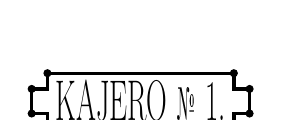
\begin{tikzpicture}[every node/.style={inner sep=0pt}]
\node[align=center](Text){\scalebox{0.5}[1]{\huge{\copperfont{KAJERO}} {\LARGE \textnumero} \copperfont 1.}};
\coordinate[shift={(-0.1cm,0.1cm)}](A) at (Text.north west);
\coordinate[shift={(0.1cm,0.1cm)}](B) at (Text.north east);
\coordinate[shift={(0.1cm,-0.1cm)}](C) at (Text.north east);
\coordinate[shift={(0.3cm,-0.1cm)}](D) at (Text.north east);
\coordinate[shift={(0.3cm,0.1cm)}](E) at (Text.south east);
\coordinate[shift={(0.1cm,0.1cm)}](F) at (Text.south east);
\coordinate[shift={(0.1cm,-0.1cm)}](G) at (Text.south east);
\coordinate[shift={(-0.1cm,-0.1cm)}](H) at (Text.south west);
\coordinate[shift={(-0.1cm,0.1cm)}](I) at (Text.south west);
\coordinate[shift={(-0.3cm,0.1cm)}](J) at (Text.south west);
\coordinate[shift={(-0.3cm,-0.1cm)}](K) at (Text.north west);
\coordinate[shift={(-0.1cm,-0.1cm)}](L) at (Text.north west);
\draw[very thick](A) -- (B) -- (C) -- (D) -- (E) -- (F) -- (G) -- (H) -- (I) -- (J) -- (K) -- (L) -- cycle;
\filldraw(A) circle [radius=1.25pt];
\filldraw(B) circle [radius=1.25pt];
\filldraw(D) circle [radius=1.25pt];
\filldraw(E) circle [radius=1.25pt];
\filldraw(G) circle [radius=1.25pt];
\filldraw(H) circle [radius=1.25pt];
\filldraw(J) circle [radius=1.25pt];
\filldraw(K) circle [radius=1.25pt];
\end{tikzpicture}}

% the command for the morpheme-separation stroke
%
\renewcommand{\,}{\raisebox{-1.1ex}{\relsize{-0.5}{\textquotesingle}}}

% displays the "RO." in "DRO." on the title page raised and underlined
%
\newcommand{\doktororo}{\setul{3pt}{.4pt}\setbox0=\hbox{X}\belowbaseline[-1.2ex]{\ul{\small RO}}}

% litera spaco
%
\sodef\spaceout{}{.2em}{0.6em}{0pt}
\sodef\spaceoutmed{}{.1em}{0.5em}{0pt}

% bookmarks
%
\usepackage{bookmark}

%
% End preamble and then begin title page
% 
\begin{document}
\sloppy
\begin{titlepage}

\newlength{\tempparskip}
\setlength{\tempparskip}{\parskip}
\setlength{\parskip}{2ex}
\newlength{\tempparindent}
\setlength{\tempparindent}{\parindent}

\vspace*{\fill}

\begin{center}
\scalebox{0.8}[1]{\latinia{\LARGE D\doktoror{} ESPERANTO’S}}

\scalebox{1}[3]{\didone{\LARGE INTERNATIONAL LANGUAGE,}}

{\sansfont{\LARGE INTRODUCTION}}

{\Large \&}

\scalebox{1.8}[1.8]{\shadowtext{\cowboyfont{\LARGE Complete\hspace{1ex}Grammar.}}}

\poranglojbox

\scalebox{0.45}[1]{\copper{\huge ENGLISH EDITION}}

{\small BY}

\scalebox{1.5}[0.7]{\cowboyfont{\LARGE R. H. Geoghegan}}

\scalebox{1}[0.7]{\monastic{\large Balliol College, Oxford.}}\\[1ex]
\pgfornament[width=0.4\textwidth]{89}

\scalebox{0.8}[1]{\large \angloj{WARSAW.}}

\scalebox{1.5}[0.7]{\cowboyfont{\Large L. Samenhof, Przejazd N. 9.}}

\rule{3em}{0.4pt}

\scalebox{1.5}[1]{{1889.}}

\vspace*{\fill}

\end{center}

\setlength{\parskip}{\tempparskip}
\end{titlepage}

%
% Inside title page
%
\renewcommand{\footrulewidth}{0.4pt}
\setstretch{1.1}

\vspace*{12em}

\begin{table}[h]
\begin{center}
{ДОЗВОЛЕНО ЦЕНЗУРОЮ \\
\vspace{1ex}
Варшава, 5 Января 1889 года.}
\end{center}

\end{table}

\vspace{5em}

{\small \finger An international language, like every national one, is the property of society, and the author renounces all personal rights in it forever.}

\vspace{5em}

\begin{flushright}
\begin{tabular}{r}
\hline
\bf\footnotesize Printed by Ch. Kelter Nowolipie Str. N. 11.
\end{tabular}
\end{flushright}

\setlength{\parskip}{0pt}

\vspace*{\fill}

%
% Introduction
%
\titleformat{\chapter}[display]{\centering}{\chaptertitlename}{0pt}{\Huge}
\renewcommand{\footrulewidth}{0pt}
\chapter*{\scalebox{0.8}[1]{INTRODUCTION.}}
\fancyhead[C]{--- \thepage{} ---}

\begin{center}
\rule{5em}{0.4pt}
\end{center}

The reader will doubtless take up this little work with an incredulous smile, supposing that he is about to peruse the impracticable schemes of some good citizen of Utopia. I would, therefore, in the first place, beg of him to lay aside all prejudice, and treat seriously and critically the question brought before him.

I need not here point out the considerable importance to humanity of an international language,---a language unconditionally accepted by everyone, and the common property of the whole world. How much time and labour we spend in learning foreign tongues, and yet when travelling in foreign countries, we are, as a rule, unable to converse with other human beings in their own language. How much time, labour, and money are wasted in translating the literary productions of one nation into the language of another, and yet, if we rely on translations alone, we can become acquainted with but a tithe of foreign literature.

Were there but an international language, all translations would be made into it alone, as into a tongue intelligible to all, and works of an international character would be written in it in the first instance.

The Chinese wall dividing literatures would disappear, and the works of other nations would be as readily intelligible to us as those of our own authors. Books being the same for everyone, education, ideals, convictions, aims, would be the same too, and all nations would be united in a common brotherhood. Being compelled, as we now are, to devote our time to the study of several different languages, we cannot study any of them sufficiently well, and there are but few persons who can even boast a complete mastery of their mother-tongue; on the other hand, languages cannot progress towards perfection, and we are often obliged, even in speaking our own language, to borrow words and expressions from foreigners, or to express our thoughts inexactly.

How different would the case be, had we but two languages to learn; we should know them infinitely better, and the languages themselves would grow richer, and reach a higher degrees of perfection than is found in any of those now existing. And yet, though language is the prime motor of civilisation, and to it alone we owe the having raised ourselves above the level of other animals, difference of speech is a cause of antipathy, nay even of hatred, between people, as being the first thing to strike us on meeting. Not being understood we keep aloof, and the first notion that occurs to our minds is, not to find out whether the others are of our own political opinions, or whence their ancestors came from thousands of years ago, but to dislike the strange sound of their language. Any one, who has lived for a length of time in a commercial city, whose inhabitants were of different unfriendly nations, will easily understand what a boon would be conferred on mankind by the adoption of an international idiom, which, without interfering with domestic affairs or the private-life of nations, would play the part of an official and commercial dialect, at any rate in countries inhabited by people of different nationalities.

The immense importance, which it may well be imagined, an international language would acquire in science, commerce, etc., I will not here expatiate on: whoever has but once bestowed a thought on the subject will surely acknowledge that no sacrifice would be too great, if by it we could obtain a universal tongue. It is, therefore, imperative that the slightest effort in that direction should be attended to. The best years of my life have been devoted to the momentous cause which I am now bringing before the public, and I hope that, on account of the importance of the subject, my readers will peruse this pamphlet attentively to the end.

I shall not here enter upon an analysis of the various attempts already made to give the public a universal language, but will content myself with remarking that these efforts have amounted, either to a short system of mutually-intelligible signs, or to a natural simplification of the grammar of existing modern languages, with a change of their words into arbitrarily-formed ones. The attempts of the first category were quickly seen to be too complicated for practical use, and so faded into oblivion; those of the second were, perhaps, entitled to the name of “languages”, but certainly not “international” languages. The inventors called their tongues “universal”, I know not why, possibly, because no one in the whole world except themselves could understand a single word, written or spoken in any of them. If a language, in order to become universal, has but to be named so, then, forsooth, the wish of any single individual can frame out of any existing dialect a universal tongue. As these authors na\"{i}vely imagined that their essays would be enthusiastically welcomed and taken up by the whole world, and as this unanimous welcome is precisely what the cold and indifferent world declines to give, when there is no chance of realising any immediate benefit, it is not much to be marvelled at, if these brilliant attempts came to nothing. The greater part of the world was not in the slightest degree interested in the prospect of a new language, and the persons who really cared about the matter thought it scarcely worth while to learn a tongue which none but the inventor could understand. When the whole world, said they, has learnt this language, or at least several million people, we will do the same. And so a scheme, which had it but been able to number some thousands of adepts before its appearance in public, would have been enthusiastically hailed, came into the world an utter fiasco. If the \glqq{}Volapük\grqq{}, one of the latest attempts at a universal tongue, has indeed its adepts, it owes its popularity solely to the idea of its being a “universal language”, and that idea has in itself something so attractive and sublime, that true enthusiasts, leaders in every new discovery, are ready to devote their time, in the hope that they may, perchance, win the cause.

But the number of enthusiasts, after having risen to a certain number, will remain stationary\footnote{One cannot, of course, reckon the number of those who learned the language as equal to the number of instruction-books sold.} and as the unfeeling and indifferent world will never consent to take any pains in order to speak with the few, this attempt will, like its predecessors, disappear without having achieved any practical victory.

I have always been interested in the question of a universal language, but as I did not feel myself better qualified for the work than the authors of so many other fruitless attempts, I did not risk running into print, and merely occupied myself with imaginary schemes and a minute study of the problem. At length, however, some happy ideas, the fruits of my reflections, incited me to further work, and induced me to essay the systematic conquest of the many obstacles, which beset the path of the inventor of a new rational universal language. As it appears to me that I have almost succeeded in my undertaking, I am now venturing to lay before the critical public, the results of my long and assiduous labours.

The principal difficulties to be overcome were:

1) To render the study of the language so easy as to make its acquisition mere play to the learner.

2) To enable the learner to make direct use of his knowledge with persons of any nationality, whether the language be universally accepted or not; in other words, the language is to be directly a means of international communication.

3) To find some means of overcoming the natural indifference of mankind, and disposing them, in the quickest manner possible, and \emph{en masse}, to learn and use the proposed language as a living one, and not only in last extremities, and with the key at hand.

Amongst the numberless projects submitted at various times to the public, often under the high-sounding but unaccountable name of “universal languages”, no one has solved at once more than \inbold{one} of the above-mentioned problems, and even that but partially. (Many other problems, of course, presented themselves, in addition to those here noticed, but these, as being of but secondary importance, I shall not in this place discuss).

Before proceeding to enlighten the reader as to the means employed for the solution of the problems, I would ask of him to reconsider the exact significance of each separately, so that he may not be inclined to carp at my methods of solution, merely because they may appear to him perhaps too simple. I do this, because I am well aware that the majority of mankind feel disposed to bestow their consideration on any subject the more carefully, in proportion as it is enigmatical and incomprehensible. Such persons, at the sight of so short a grammar, with rules so simple, and so readily intelligible, will be ready to regard it with a contemptuous glance, never considering the fact, --- of which a little further reflection would convince them, --- that this simplification and bringing of each detail out of its original complicated form into the simplest and easiest conceivable, was, in fact, the most insuperable obstacle to be coped with. 

\vspace{12pt}

{\hfil \scalebox{2}[1]{\large\cowboyfont I.}}

\vspace{12pt}

The first of the problems was solved in the following manner:

1) I simplified the grammar to the utmost, and while, on the one hand, I carried out my object in the spirit of the existing modern languages, in order to make the study as free from difficulties as possible, on the other hand I did not deprive it of clearness, exactness, and flexibility. My whole grammar can be learned perfectly in \inbold{one hour}. The immense alleviation given to the study of a language, by such a grammar, must be self-evident to everyone.

2) I established rules for the formation of new words, and at the same time, reduced to a very small compass the list of words absolutely necessary to be learned, without, however, depriving the language of the means of becoming a rich one. On the contrary, thanks to the possibility of forming from one root-word any number of compounds, expressive of every conceivable shade of idea, I made it the richest of the rich amongst modern tongues. This I accomplished by the introduction of numerous prefixes and suffixes, by whose aid the student is enabled to create new words for himself, without the necessity of having previously to learn them, e.~g.

1) The prefix \emph{mal} denotes the direct opposite of any idea. If, for instance, we know the word for “good”, \emph{bon\,a}, we can immediately form that for “bad”, \emph{mal\,bon\,a}, and hence the necessity of a special word for “bad” is obviated. In like manner, \emph{alt\,a}, “high”, “tall”, \emph{mal\,alt\,a,} “low”, “short”; \emph{estim\,i,} “to respect”, \emph{mal\,estim\,i}, “to despise”, etc. Consequently, if one has learned this single word \emph{mal} he is relieved of leaning a long string of words such as “hard” (premising that he knows “soft”), “cold”, “old”, “dirty”, “distant”, “darkness”, “shame”, “to hate”, etc., etc.

2) The suffix \emph{in} marks the feminine gender, and thus if we know the word “brother”, \emph{frat\,o}, we can form “sister”, \emph{frat\,in\,o}: so also, “father”, \emph{patr\,o}; “mother”, \emph{patr\,in\,o}. By this device words like “grandmother”, “bride”, “girl”, “hen”, “cow”, etc., are done away with.

3) The suffix \emph{il} indicates an instrument for a given purpose, e.~g., \emph{tranĉ\,i}, “to cut”, \emph{tranĉ\,il\,o}, “a knife”; so words like “comb”, “axe”, “bell”, etc., are rendered unnecessary.

In the same manner are employed many other affixes, --- some fifty in all, --- which the reader will find in the vocabulary at end of this tractate.\footnote{To facilitate the finding of these affixes they are entered in the vocabulary as separate words.} Moreover, as I have laid it down as a general rule, that every word already regarded as international, --- the so-called “foreign” words, for example, --- undergoes no change in my language, except such as may be necessary to bring it into conformity with the international orthography, innumerable words become superfluous, e.~g., “locomotive”, “telegraph”, “nerve”, “temperature”, “centre”, “form”, “public”, “platinum”, “figure”, “waggon”, “comedy”, and hundreds more.

By the help of these rules, and others, which will be found in the grammar, the language is rendered so exceedingly simple that the whole labour in learning consists in committing to memory some 900 words, --- which number includes all the grammatical inflexions, prefixes, etc. --- With the assistance of the rules given in the grammar, any one of ordinary intellectual capacity, may form for himself all the words, expressions, and idioms in ordinary use. Even these 900 words, as will be shown directly, are so chosen, that the learning them offers no difficulty to a well-educated person.

Thus the acquirement of this rich, mellifluous, universally-comprehensible language, is not a matter of years of laborious study, but the mere light amusement of a few days. 

\vspace{12pt}

{\hfil \scalebox{2}[1]{\large\cowboyfont II.}}

\vspace{12pt}

The solution of the second problem was effected thus:

1) I introduced a complete dismemberment of ideas into independent words, so that the whole language consists, not of words in different states of grammatical inflexion, but of unchangeable words. If the reader will turn to one of the pages of this book written in my language, he will perceive that each word always retains its original unalterable form, ---namely, that under which it appears in the vocabulary. The various grammatical inflexions, the reciprocal relations of the members of a sentence, are expressed by the junction of immutable syllables. But the structure of such a synthetic language being altogether strange to the chief European nations, and consequently difficult for them to become accustomed to, I have adapted this principle of dismemberment to the spirit of the European languages, in such a manner that anyone learning my tongue from grammar alone, without having previously read this introduction, --- which is quite unnecessary for the learner, --- will never perceive that the structure of the language differs in any respect from that of his mother-tongue. So, for example, the derivation of \emph{frat\,in\,o}, which is in reality a compound of \emph{frat} “child of the same parents as one’s self”, \emph{in} “female”, \emph{o} “an entity”, “that which exists”, i.~e., “that which exists as a female child of the same parents as one’s self” = “a sister”,--- is explained by the grammar thus: the root for “brother” is \emph{frat}, the termination of substantives in the nominative case is \emph{o}, hence \emph{frat\,o} is the equivalent of “brother”; the feminine gender is formed by the suffix \emph{in}, hence \emph{frat\,in\,o} = “sister”. (The little strokes, between certain letters, are added in accordance with a rule of the grammar, which requires their insertion between each component part of every complete word). Thus the learner experiences no difficulty, and never even imagines that what he calls terminations, suffixes, etc.,---are complete and independent words, which always keep their own proper significations, whether placed at the beginning or end of a word, in the middle, or alone. The result of this construction of the language is, that everything written in it can be immediately and perfectly understood by the help of the vocabulary, --- or even almost without it, --- by anyone who has not only not learnt the language before, but even has never heard of its very existence. Let me illustrate this by an example: --- I am amongst Englishmen, and have not the slightest knowledge of the English language; I am absolutely in need of making myself understood, and write in the international tongue, may be, as follows:

    \emph{Mi ne sci\,as ki\,e mi las\,is la baston\,o\,n; ĉu vi ĝi\,n ne vid\,is?}

I hold out to one of the strangers an International--English vocabulary, and point to the title, where the following sentence appears in large letters: “Everything written in the international language can be translated by the help of this vocabulary. If several words together express but a single idea, they are written as one word, but separated by commas; e.~g., \emph{frat\,in\,o}, though a single idea is yet composed of three words which must be looked for separately in the vocabulary”. If my companion has never heard of the international language he will probably favour me at first with a vacant stare, will then take the paper offered to him, and searching for the words in the vocabulary, as directed, will make out something of this kind:

\smaller

\begingroup
\renewcommand{\arraystretch}{1}
\begin{longtable}{>{\itshape}c@{ }l@{ }>{\itshape}l>{\ttfamily}l@{ }p{4cm}@{ }l@{ }c}
Mi & \tlba & mi & = & I & \trba & I \\
ne & \tlba & ne & = & not & \trba & not \\
\multirow{2}{*}{sci\,as} & \tlbb & sci & = & know & \trbb & \multirow{2}{*}{do know} \\
 & & as & = & sign of the present tense \\
kie & \tlba & kie & = & where & \trba & where \\
mi & \tlba & mi & = & I & \trba & I \\
\multirow{2}{*}{las\,is} & \tlbb & las & = & leave & \trbb & \multirow{2}{*}{have left} \\
 & & is & = & sign of the past tense \\
la & \tlba & la & = & the & \trba & the \\
\multirow{3}{*}{baston\,o\,n;} & \tlbc & baston & = & stick & \trbc & \multirow{3}{*}{stick;} \\
 & & o & = & sign of a substantive \\
 & & n & = & sign of the objective case \\
\multirow{2}{*}{ĉu} & \tlbb & ĉu & = & {whether, if, employed in questions} & \trbb & \multirow{2}{*}{whether} \\
vi & \tlba & vi & = & you, thou & \trba & you \\
\multirow{2}{*}{ĝi\,n} & \tlbb & ĝi & = & it, this & \trbb & \multirow{2}{*}{it} \\
 & & n & = & sign of the objective case \\
ne & \tlba & ne & = & not & \trba & not \\
\multirow{2}{*}{vid\,is?} & \tlbb & vid & = & see & \trbb & \multirow{2}{*}{have seen?} \\
 & & is & = & sign of the past tense \\
\end{longtable}
\endgroup
\normalsize
And thus the Englishman will easily understand what it is I desire. If he wishes to reply, I show him an English--International vocabulary, on which are printed these words: “To express anything by means of this vocabulary, in the international language, look for the words required, in the vocabulary itself; and for the terminations necessary to distinguish the grammatical forms, look in the grammatical appendix, under the respective headings of the parts of speech which you desire to express”. Since the explanation of the whole grammatical structure of the language is comprised in a few lines,---as a glance at the grammar will show,---the finding of the required terminations occupies no longer time than the turning up a word in the dictionary.

I would now direct the attention of my readers to another matter, at first sight a trifling one, but, in truth, of immense importance. Everyone knows the impossibility of communicating intelligibly with a foreigner, by the aid of even the best of dictionaries, if one has no previous acquaintance with the language. In order to find any given word in a dictionary, we must know its derivation, for when words are arranged in sentences, nearly every one of them undergoes some grammatical change. After this alteration, a word often bears not the least resemblance to its primary form, so that without knowing something of the language beforehand, we are able to find hardly any of the words occurring in a given phrase, and even those we do find will give no connected sense. Suppose, for example, I had written the simple sentence adduced above, in German: \glqq Ich weiss nicht wo ich den Stock gelassen habe; haben Sie ihn nicht gesehen?\grqq{} Anyone who did not speak or understand German, after searching for each word separately in a dictionary, would produce the following farrago of nonsense: “I; white; not; where; I; --- ; stick; dispassionate; property; to have; she, they, you; --- ; not; --- ?” I need scarcely point out that a lexicon of a modern language is usually a tome of a certain bulk, and the search for any number of words one by one is in itself a most laborious undertaking, not to speak of the different significations attaching to the same word amongst which there is but a bare possibility of the student selecting the right one. The international vocabulary, owing to the highly synthetic structure of the language, is a mere leaflet, which one might carry in one’s note-book, or the waistcoat-pocket. Granted that we \emph{had} a language with a grammar simplified to the utmost, and whose every word had a definite fixed meaning, the person addressed would require not only to have beforehand some knowledge of the grammar, to be able, even with the vocabulary at hand, to understand anything addressed to him, but would also need some previous acquaintance with the vocabulary itself, in order to be able to distinguish between the primitive word and its grammatically-altered derivatives. The utility, again, of such a language would wholly depend upon the number of its adepts, for when sitting, for instance, in a railway-carriage, and wishing to ask a fellow-traveller, “How long do we stop at ---?”, it is scarcely to be expected that he will undertake to learn the grammar of the language before replying! By using, on the other hand, the international language, we are set in possibility of communicating directly with a person of any nationality, even though he may never have heard of the existence of the language before.

Anything whatever, written in the international tongue, can be translated, without difficulty, by means of the vocabulary alone, no previous study being requisite. The reader may easily convince himself of the truth of this assertion, by experimenting for himself with the specimens of the language appended to this pamphlet. A person of good education will seldom need to refer to the vocabulary, a linguist scarcely at all.

Let us suppose that you have to write to a Spaniard, who neither knows your language nor you his. You think that probably he has never heard of the international tongue. --- No matter, write boldly to him in that language, and be sure he will understand you perfectly. The complete vocabulary required for everyday use, being but a single sheet of paper, can be bought for a few pence, in any language you please, easily enclosed in the smallest envelope, and forwarded with your letter. The person to whom it is addressed will without doubt understand what you have written, the vocabulary being not only a clue to, but a complete explanation of your letter. The wonderful power of combination possessed by the words of the international language renders this lilliputian lexicon amply sufficient for the expression of every want of daily life; but words seldom met with, technical terms, and foreign words familiar to all nations, as, “tobacco”, “theatre”, “fabric”, etc., are not included in it. If such words, therefore, are needed, and it is impossible to express them by some equivalent terms, the larger vocabulary must be consulted.

2) It has now been shown how, by means of the peculiar structure of the international tongue, any one may enter into an intelligible correspondence with another person of a different nationality. The sole drawback, until the language becomes more widely known, is the necessity under which the writer is placed of waiting until the person addressed shall have analysed his thoughts. In order to remove this obstacle, as far as practicable, at least for persons of education, recourse was had to the following expedient. Such words as are common to the languages of all civilised peoples, together with the so-called “foreign” words, and technical terms, were left unaltered. If a word has a different sound in different languages, that sound has been chosen which is common to at least two or three of the most important European tongues, or which, if found in one language only, has become familiar to other nations. When the required word has a different sound in every language, some word was sought for, having only a relative likeness in meaning to the other, or one which, though seldom used, is yet well-known to the leading nations, e.~g., the word for ``near'' is different in every European language, but if one consider for a moment the word ``proximus'' (nearest), it will be noticed that some modified form of the word is in use in all important tongues. If, then, I call ``near'', \emph{proksim}, the meaning will be apparent to every educated man. In other emergencies words were drawn from the Latin, as being a quasi-international language. Deviations from these rules were only made in exceptional cases, as for the avoidance of homonyms, simplicity of orthography, etc. In this manner, being in communication with a European of fair education, who has never learnt the international tongue, one may make sure of being immediately understood, without the person addressed having to refer continually to the vocabulary.

In order that the reader may prove for himself the truth of all that has been set forth above, a few specimens of the international language are subjoined.\footnote{In correspondence with persons who have learnt the language, as well as in works written for them exclusively, the commas, separating parts of words, are omitted.}


\secthead{Patr\,o ni\,a.}{2ex}{2ex}

Patr\,o ni\,a, kiu est\,as en la ĉiel\,o, sankt\,a est\,u Vi\,a nom\,o, ven\,u reĝ\,ec\,o Vi\,a, est\,u vol\,o Vi\,a, kiel en la ĉiel\,o, tiel ankaŭ sur la ter\,o. Pan\,o\,n ni\,a\,n ĉiu\,tag\,a\,n don\,u al ni hodiaŭ, kaj pardon\,u al ni ŝuld\,o\,j\,n ni\,a\,j\,n, kiel ni ankaŭ pardon\,as al ni\,a\,j ŝuld\,ant\,o\,j; ne konduk\,u ni\,n en tent\,o\,n; sed liber\,ig\,u ni\,n de la mal\,ver\,a, ĉar Vi\,a est\,as la reg\,ad\,o, la fort\,o, kaj la glor\,o etern\,e. Amen!


\secthead{El la Bibli\,o.}{2ex}{2ex}

Je la komenc\,o Di\,o kre\,is la ter\,o\,n kaj la ĉiel\,o\,n. Kaj la ter\,o est\,is sen\,form\,a kaj dezert\,a, kaj mal\,lum\,o est\,is super la profund\,aĵ\,o, kaj la anim\,o de Di\,o si\,n port\,is super la akv\,o. Kaj Di\,o dir\,is: est\,u lum\,o; kaj far\,iĝ\,is lumo. Kaj Di\,o vid\,is la lum\,o\,n ke ĝi est\,as bon\,a, kaj nom\,is Di\,o la lum\,o\,n tag\,o, kaj la mal\,lum\,o\,n Li nom\,is nokt\,o. Kaj est\,is vesper\,o, kaj est\,is maten\,o --- unu tag\,o. Kaj Di\,o dir\,is: est\,u firm\,aĵ\,o inter la akv\,o, kaj ĝi apart\,ig\,u akv\,o\,n de akv\,o. Kaj Di\,o kre\,is la firm\,aĵ\,o\,n kaj apart\,ig\,is la akv\,o\,n kiu est\,as sub la firm\,aĵ\,o, de la akv\,o kiu est\,as super la firm\,aĵ\,o; kaj far\,iĝ\,is tiel. Kaj Di\,o nom\,is la firm\,aĵ\,o\,n ĉiel\,o. Kaj est\,is vesper\,o, kaj est\,is maten\,o --- la du\,a tag\,o. Kaj Di\,o dir\,is: kolekt\,u si\,n la akv\,o de sub la ĉiel\,o unu lok\,o\,n, kaj montr\,u si\,n sek\,aĵ\,o; kaj far\,iĝ\,is tiel. Kaj Di\,o nom\,is la sek\,aĵ\,o\,n ter\,o, kaj la kolekt\,oj\,n de la akv\,o Li nom\,is mar\,o\,j.

\secthead{Leter\,o.}{2ex}{2ex}

\hspace{5em} Kar\,a amik\,o!

Mi prezent\,as al mi kia\,n vizaĝ\,o\,n vi far\,os post la ricev\,o de mi\,a leter\,o. Vi rigard\,os la sub\,skrib\,o\,n kaj ek\,kri\,os: “ĉu li perd\,is la saĝ\,o\,n? Je kia lingv\,o li skrib\,is? Kio\,n signif\,as la foli\,et\,o, kiu\,n li al\,don\,is al si\,a leter\,o?” Trankvil\,iĝ\,u, mi\,a kar\,a! Mi\,a saĝ\,o, kiel mi almenaŭ kred\,as, est\,as tut\,e en ord\,o.

Mi leg\,is antaŭ kelk\,a\,j tag\,o\,j libr\,et\,o\,n sub la nom\,o \glqq{}Lingv\,o inter\,naci\,a\grqq{}. La aŭtor\,o kred\,ig\,as, ke per tiu lingv\,o oni pov\,as est\,i kompren\,at\,a de la tut\,a mond\,o, se eĉ la adres\,it\,o ne sol\,e ne sci\,as la lingv\,o\,n, sed eĉ ankaŭ ne aŭd\,is pri ĝi; oni dev\,as sol\,e al\,don\,i al la leter\,o mal\,grand\,a\,n foli\,et\,o\,n nom\,at\,a\,n \glqq{}vort\,ar\,o\grqq{}. Dezir\,ant\,e vid\,i, ĉu tio est\,as ver\,a, mi skrib\,as al vi en tiu lingv\,o, kaj mi eĉ unu vort\,o\,n ne al\,met\,as en ali\,a lingv\,o, tiel kiel se ni tut\,e ne kompren\,us unu la lingv\,o\,n de la ali\,a. Respond\,u al mi, ĉu vi efektiv\,e kompren\,is kio\,n mi skrib\,is. Se la afer\,o propon\,it\,a de la aŭtor\,o est\,as efektiv\,e bon\,a, oni dev\,as per ĉiu\,j fort\,o\,j li\,n help\,i. Kiam mi hav\,os vi\,a\,n respond\,o\,n, mi send\,os al vi la libr\,et\,o\,n; montr\,u ĝi\,n al ĉiu\,j loĝ\,ant\,o\,j de vi\,a urb\,et\,o, send\,u ĝin ĉiu\,n vilaĝ\,o\,n ĉirkaŭ la urb\,et\,o, ĉiu\,n urb\,o\,n kaj urb\,et\,o\,n, kie vi nur hav\,as amik\,o\,j\,n aŭ kon\,at\,o\,j\,n. Est\,as neces\,e ke grand\,eg\,a nombr\,o da person\,o\,j don\,u si\,a\,n voĉ\,o\,n --- tiam post la plej mal\,long\,a temp\,o est\,os decid\,it\,a afer\,o, kiu pov\,as port\,i grand\,eg\,a\,n util\,o\,n al la hom\,a societ\,o.

\secthead{Mi\,a pens\,o.}{2ex}{0pt}

\begin{verse}
        \hspace{1em} Sur la kamp\,o, for de l’mond\,o,\\
        Antaŭ nokt\,o de somer\,o\\
        Amik\,in\,o en la rond\,o\\
        Kant\,as kant\,o\,n pri l’esper\,o.\\
        Kaj pri viv\,o detru\,it\,a\\
        Ŝi rakont\,as kompat\,ant\,e, ---\\
        Mi\,a vund\,o re\,frap\,it\,a\\
        Mi\,n dolor\,as re\,sang\,ant\,e.\\

\pstars

        \hspace{1em} \glqq{}Ĉu vi dorm\,as? Ho, sinjor\,o,\\
        Kial tia sen\,mov\,ec\,o?\\
        Ha, kred\,ebl\,e re\,memor\,o\\
        El la kar\,a infan\,ec\,o?\grqq{}\\
        Kio\,n dir\,i? Ne plor\,ant\,a\\
        Pov\,is est\,i parol\,ad\,o\\
        Kun fraŭl\,in\,o ripoz\,ant\,a\\
        Post somer\,a promen\,ad\,o!\\

\pstars

        \hspace{1em} Mi\,a pens\,o kaj turment\,o,\\
        Kaj dolor\,o\,j kaj esper\,o\,j!\\
        Kiom de mi en silent\,o\\
        Al vi ir\,is jam ofer\,o\,j!\\
        Kio\,n hav\,is mi plej kar\,a\,n ---\\
        \emph{La jun\,ec\,o\,n} --- mi plor\,ant\,a\\
        Met\,is mem sur la altar\,o\,n\\
        De la dev\,o ordon\,ant\,a!\\

\pstars

        \hspace{1em} Fajr\,o\,n sent\,as mi intern\,e,\\
        Viv\,i ankaŭ mi dezir\,as, ---\\
        Io pel\,as mi\,n etern\,e,\\
        Se mi al gaj\,ul\,o\,j ir\,as \ldots{} \\
        Se ne plaĉ\,as al la sort\,o\\
        Mi\,a pen\,o kaj labor\,o ---\\
        Ven\,u tuj al mi la mort\,o,\\
        En esper\,o --- sen dolor\,o!
\end{verse}

\secthead{El Heine’.}{0pt}{0pt}

\begin{verse}
        \hspace{1em} En sonĝ\,o princ\,in\,o\,n mi vid\,is\\
        Kun vang\,o\,j mal\,sek\,a\,j de plor\,o, ---\\
        Sub arb\,o, sub verd\,a ni sid\,is\\
        Ten\,ant\,e si\,n kor\,o ĉe kor\,o.\\

\pstars

        \hspace{1em} \glqq{}De l’patr\,o de l’vi\,a la kron\,o\\
        Por mi ĝi ne est\,as hav\,ind\,a;\\
        For, for li\,a sceptr\,o kaj tron\,o ---\\
        Vi\,n mem mi dezir\,as, am\,ind\,a!\grqq{}\\

\pstars

        \hspace{1em} --- \glqq{}Ne ebl\,e!\grqq{} ŝi al mi re\,dir\,as:\\
        \glqq{}En tomb\,o mi est\,as ten\,at\,a,\\
        Mi nur en la nokt\,o el\,ir\,as\\
        Al vi, mi\,a sol\,e am\,at\,a!\grqq{}\\
\end{verse}

\secthead{Ho, mi\,a kor’.}{0pt}{0pt}

\begin{verse}
\hspace{1em} Ho, mi\,a kor’, ne bat\,u mal\,trankvil\,e. \\
El mi\,a brust\,o nun ne salt\,u for! \\
Jam ten\,i mi\,n ne pov\,as mi facil\,e \\
Ho, mi\,a kor’! \\

\pstars

\hspace{1em} Ho, mi\,a kor’! Post long\,a labor\,ad\,o \\
Ĉu mi ne venk\,os en decid\,a hor’! \\
Sufiĉ\,e! trankvil\,iĝ\,u de l’bat\,ad\,o, \\
Ho, mi\,a kor’! 
\end{verse}
\begin{center}
\sectionline
\vspace{12pt}
\end{center}

\hspace*{\fill}\scalebox{2}[1]{\large\cowboyfont{}III.}\hspace*{\fill}

\vspace{12pt}
\nopagebreak
I have now completed my analysis of the more remarkable features of my international language. I have shown the advantages to be derived from a study of it, and proved that its ultimate success is altogether independent of the opinions that may be formed as to its right to the title “international”. For even should the language never come into general use, it gives to every one who \emph{has} learned it, the possibility of being understood by foreigners, if only they be able to read and write. But my tongue has yet another object; not content with internationality, it aims at universality, and aspires to being \emph{spoken} by the majority of educated people. To count on the aid of the public in a scheme of this nature would indeed be to build on a tottering, --- nay rather, an imaginary, --- foundation. The larger part of the public does not care to aid anyone, it prefers to have its wishes gratified without inconvenience to itself. On this account I made my best endeavours to discover some means of accomplishing my object, independently of the help of the public. One of my plans, of which I shall now speak more at large, is a kind of “universal vote”.

If the reader consider all that has been said above, he must come to the conclusion that the study of the international language is practically useful, and completely remunerates the learner for the small amount of trouble he has to expend on it. For my own part, I am naturally wishful that the whole of mankind should take up my language, but I had rather be prepared for the worst, than form too sanguine anticipations. I suppose therefore, that, just at first, very few will consider my language worth the learning, so far as practical usefulness is concerned, and for abstract principles no one will lose even a single hour.

Most of my readers will, either pay not the slightest attention to my proposition, or, doubting whether the language be of any use, never “screw up their courage to the sticking-point” of learning it, fearing that they may be dubbed “dreamers”, a sobriquet dreaded by most people more than fire. What, then, is to be done, to dispose this mass of indifferent and undecided beings to master the international language? Could we, in imagination, look for a moment into the mind of each of these indifferent ones, we should find their thoughts to be taking somewhat of the following form. In principle, no one has anything to oppose to the introduction of an international dialect; on the contrary, all would give it their fullest approval, but each wishes to see the greater part of the civilized world able to speak the language, and himself able to comprehend it, without any preliminary “wearisome bitterness of learning”, on his own part. \emph{Then}, of course, even the most indifferent would set to work, because to shirk the small amount of labour necessary for learning a language possessed of such valuable qualities, and above all, considered \emph{``the thing''} by all the educated, would be regarded as simple stupidity.

In order to supply a language ready for immediate use, without any one having to initiate the study, and to see on every hand people either already proficient in the tongue, or having promised to take it up, we must proceed somewhat in the following manner. Doubtless this little book will be scattered through various countries, and fall into the hands of various readers. I do not ask any of my readers to spend time, labour, or money on the subject now brought to their notice. I merely beg of you, the present reader of the pamphlet, to take up your pen for a moment, fill in one of the appended \emph{\glqq Promes\,o\,j\grqq} (below) and send it to me (Dr. Esperanto, $\mathrm{^c\!/\!_o}$ Dr. L. Samenhof. Warsaw, Poland). The \emph{\glqq Promes\,o\grqq} is to this effect:

\begin{adjustwidth}{1cm}{1cm}
\hspace{1.5em} “I, the undersigned, promise to learn the international language, proposed by Dr. Es\-per\-anto, if it shall be shown that ten million similar promises have been publicly given”.
\end{adjustwidth}

If you have any objections to make to the present form of the language, strike out the words of the promise, and write \emph{\glqq kontraŭ\grqq} (against), beneath them. If you undertake to learn the language unconditionally, i.~e., without reference to the number of other students, strike out the latter words of the \glqq Promes\,o\grqq, and write \emph{\glqq{}sen\,kondiĉ\,e\grqq{}}, (unconditionally). On the back of the promise write name and address. The signing of this promise lays no obligations upon the person signing, and does not bind him to the smallest sacrifice or work. It merely puts him under an obligation to study the language, when ten million other persons shall be doing the same. When that time arrives, there will be no talking about ``sacrifice'', everyone will be ready to study the language, without having signed any promises.

On the other hand, every person signing one of these \glqq{}Promes\,o\,j\grqq{}, will, --- without any greater inconvenience to himself than dipping a pen in ink, --- be hastening on the realization of the traditional ideal of mankind, the universal language. When the number of promises has reached ten millions, a list of the names of those who have signed will be published, and with it, the question of an international language --- decided.

Nothing actually \emph{prevents} people from inducing their friends and acquaintances to sign a promise in any cause, yet how few, as a fact, ever do sign anything, be the object ever so important and advantageous to mankind. More especially, when, as in the present instance, the act of signing, while contributing to the realization of a sublime ideal, at the same time requires no moral nor material sacrifice, can one see no very clear grounds for a refusal.

Doubtless, no one has anything to say, in general, against the introduction of an international language; but, if anyone does not approve of the present form of the language, by all means let him send me, instead of his “Promise”, his “Protest”. For it is, manifestly, the duty of every person able to read and write, of every age, sex, or profession, to give his opinion in this great undertaking; the more so, as it requires no greater sacrifice than that of a few moments for filling in the promise, and a few pence for sending it to me.

I would here beg of all editors of newspapers and magazines to make known the cause to their readers, and at the same time, I would request \emph{my} readers to mention the subject to all their friends.

I need not say any more. I am not so conceited as to suppose that my language is so perfect as to be incapable of improvement, but I make bold to think that I have satisfied all the conditions required in a language claiming to be styled “international”. It is only after having solved successfully all the problems I had proposed to myself,---concerning the more important of which only, I have been able to speak above, owing to the small compass of this pamphlet,---and after many years spent in a careful study of the subject that I venture to appear in public. I am but human; I may have erred, I may have committed unpardonable faults. I may even have omitted to give to my language the very thing most important to it. For these reasons, before printing complete vocabularies and bringing out books and magazines, I lay my work before the public, for the space of one year, addressing myself to the whole intelligent world with the earnest request to send me opinions on the proposed international language. I invite everyone to communicate with me as to the changes, corrections, etc., which he deems advisable. All such observations sent to me, I will gratefully make use of, if they appear really advantageous, and at the same time, not subversive of the fundamental principles of the structure of the language:---that is to say, simplicity, and adaptability to international communication whether adopted \emph{universally} or not.

At the end of the alloted time, an abstract of the proposed changes will be published and the language will receive its final form. But if, even then, anyone should find the language not altogether satisfactory to himself, he should not forget that the language is by no means proof against all further changes, only that the right of alteration will be no longer the author’s personal privilege, but that of an academy of the tongue.

It is no easy task to invent an international language, but it is a still less easy one to persuade the public to make use of it. Hence, it is of the utmost importance that every possible effort be made for its furtherance. When the form of the language has been decided, and the language itself has come into general use, a special academy can introduce, --- gradually and imperceptibly, --- all necessary changes, even should the result be a total alteration of the form of the language. On this account, I would pray those of my readers, who may be, for whatever reasons, dissatisfied with my language, to send in their protests only in the event of their having serious cause for it, such as the finding in the language objectionable features, unalterable in the future.

This little work, which has cost much labour and health, I now commend to the kindly attention of the public, hoping that all, to whom the public weal is dear, will aid me to the best of their ability. Circumstances will show each one in what way he can be of use; I will only direct the attention of all friends of the international language, to that most important object, towards which all eyes must be turned, the success of the voting. Let each do what he can, and in a short time we shall have, that which men have been dreaming of so long, --- \emph{``A Universal Tongue''}.

\sectionline

\newpage

\emph{NB.} The author requests his reader to fill in one of the ``Promises'' on the following page, and send it to him, and to distribute the others amongst friends and acquaintances for the same purpose.

Author's Address:

\vspace{1ex}

\hspace{1.5em} Dr. Esperanto,

\vspace{1ex}

\hspace{3em} $\mathrm{^c\!/\!_o}$ Dr. L. Samenhof,

\vspace{1ex}

\hspace{4.5em} Warsaw,

\vspace{1ex}

\hspace{6em} Russ-Poland.

\sectionline

\cleardoublepage

\begin{table}[h]
\centering
{\setlength{\extrarowheight}{2ex}%
\begin{tabular}{ccc}
\promeso{} & & \promeso \\
\promeso & & \promeso \\
\end{tabular}}
\end{table}

\begin{table}[h]
\centering
{\setlength{\extrarowheight}{2ex}%
\begin{tabular}{ccc}
\nomadreso & & \nomadreso \\
\nomadreso & & \nomadreso \\
\end{tabular}}
\end{table}


\begin{table}[h]
\centering
{\setlength{\extrarowheight}{2ex}%
\begin{tabular}{ccc}
\promeso & & \promeso \\
\promeso & & \promeso \\
\end{tabular}}
\end{table}

\begin{table}[h]
\centering
{\setlength{\extrarowheight}{2ex}%
\begin{tabular}{ccc}
\nomadreso & & \nomadreso \\
\nomadreso & & \nomadreso \\
\end{tabular}}
\end{table}

%
% Grammar
%
\titlespacing*{\chapter}{0pt}{0pt}{0pt}
\titleformat{\section}[display]{\centering}{\sectiontitlename}{0pt}{\Large}
\chapter*{\scalebox{1.5}[1.5]{\LARGE\shadowtext{\bosox{COMPLETE GRAMMAR}}}}
\begin{center}
\scalebox{0.7}[1]{\LARGE OF THE INTERNATIONAL LANGUAGE.}
\sectionline

\section*{\scalebox{0.8}[1]A. \hspace{.2em} \scalebox{0.85}{\grammarpartsfont{The \hspace{.2em} Alphabet.}}}
\setstretch{1}
\begin{tabularx}{\textwidth}{+Y@{}^Y@{}^Y@{}^Y@{}^Y@{}^Y}
\rowstyle{\LARGE} A a, & B b, & C c, & Ĉ ĉ, & D d, & E e,  \\ 
\rowstyle{\footnotesize} \emph{a} as in ``last'' & \emph{b} as in ``be'' & \emph{ts} as in ``wits'' & \emph{ch} as in ``church'' & \emph{d} as in ``do'' & \emph{e} as in ``make'' \\[3ex] 
\rowstyle{\LARGE} F f, & G g, & Ĝ ĝ, & H h, & Ĥ ĥ, & I i, \\
\rowstyle{\footnotesize} \emph{f} as in ``fly'' & \emph{g} as in ``gun'' & \emph{j} as in ``join'' & \emph{h} as in ``half'' & strongly aspirated h, \emph{ch} as in ``loch'' (Scotch) & \emph{i} as in ``marine''  \\[9ex]
\rowstyle{\LARGE} J j, & Ĵ ĵ, & K k, & L l, & M m, & N n,  \\
\rowstyle{\footnotesize} \emph{y} as in ``yoke'' & \emph{z} as in ``azure'' & \emph{k} as in ``key'' & \emph{l} as in ``line'' & \emph{m} as in ``make'' & \emph{n} as in ``now'' \\[3ex]
\rowstyle{\LARGE}O o, & P p, & R r, & S s, & Ŝ ŝ, & T t,   \\
\rowstyle{\footnotesize} \emph{o} as in ``not'' & \emph{p} as in ``pair'' & \emph{r} as in ``rare'' & \emph{s} as in ``see'' & \emph{sh} as in ``show'' & \emph{t} as in ``tea'' \\[3ex]
\rowstyle{\LARGE} & U u, & Ŭ ŭ, & V v, & Z z. \\
\rowstyle{\footnotesize} & \emph{u} as in ``bull'' & \emph{u} as in ``mount'' (used in diphthongs) & \emph{v} as in ``very'' & \emph{z} as in ``zeal'' 
\end{tabularx}
\end{center}
\setstretch{1.1}

If it be found impractical to print works with the diacritical signs ( ˆ, ˘ ), the letter \emph{h} may be substituted for the sign ( ˆ ), and the sign ( ˘ ) may be altogether omitted; but at the beginning of works so printed there should be this note: ``NB ch \texttt{=} ĉ; gh \texttt{=} ĝ; hh \texttt{=} ĥ; jh \texttt{=} ĵ; sh \texttt{=} ŝ.''

When it is necessary to make use of the ``internal'' sign ( \, ) care should be taken that it can not be mistaken for a comma.  Instead of ( \, ) may be printed ( {\relsize{-2.5}$'$} ) or ( $\cdot$ ), e.~g. \emph{sign\,et\,o, sign{\relsize{-2.5}$'$}et{\relsize{-2.5}$'$}o,} or \emph{sign$\cdot$et$\cdot$o}.

\section*{\scalebox{0.8}[1]B. \hspace{.2em} \scalebox{0.85}{\grammarpartsfont{Parts \hspace{.2em} of \hspace{.2em} Speech.}}}

1. There is no indefinite, and only one definite, article, \emph{la}, for all genders, numbers, and cases.

2. Substantives are formed by adding \emph{o} to the root. For the plural, the letter \emph{j} must be added to the singular. There are two cases: the nominative and the objective (accusative). The root with the added \emph{o} is the nominative, the objective adds an \emph{n} after the \emph{o}. Other cases are formed by prepositions; thus, the possessive (genitive) by \emph{de}, “of”; the dative by \emph{al}, “to”; the instrumental (ablative) by \emph{kun}, “with”, or other preposition as the sense demands. E.~g., root \emph{patr}, “father”; \emph{la patr\,o}, “the father”; \emph{patr\,o\,n}, “father” (objective), \emph{de la patr\,o}, “of the father”, \emph{al la patr\,o}, “to the father”, \emph{kun la patr\,o}, “with the father”; \emph{la patro\,j}, “the fathers”; \emph{la patro\,j\,n}, “the fathers” (obj.), \emph{por la patr\,o\,j}, “for the fathers”.

3. Adjectives are formed by adding \emph{a} to the root. The numbers and cases are the same as in substantives. The comparative degree is formed by prefixing \emph{pli} (more); the superlative by \emph{plej} (most). The word “than” is rendered by \emph{ol}, e.~g., \emph{pli blank\,a ol neĝ\,o}, “whiter than snow”.

4. The cardinal numerals do not change their forms for the different cases. They are:

\begin{center}
\begin{tabular}{rlccrl}
1 & \emph{unu} & \hspace{2em} & \hspace{2em} & 7 & \emph{sep} \\
2 & \emph{du} & & & 8 & \emph{ok} \\
3 & \emph{tri} & & & 9 & \emph{naŭ} \\
4 & \emph{kvar} & & & 10 & \emph{dek} \\
5 & \emph{kvin} & & & 100 & \emph{cent} \\
6 & \emph{ses} & & & 1000 & \emph{mil} 
\end{tabular}
\end{center}

The tens and hundreds are formed by simple junction of the numerals, e.~g., 533 = \emph{kvin\,cent tri\,dek tri}.

Ordinals are formed by adding the adjectival \emph{a} to the cardinals, e.~g., \emph{unu\,a}, “first”; \emph{du\,a}, “second”, etc.

Multiplicatives (as “threefold”, “fourfold”, etc.) add \emph{obl}, e.~g., \emph{tri\,obl\,a}, “threefold”.

Fractionals add \emph{on}, as \emph{du\,on\,o}, “a half”, \emph{kvar\,on,o}, “a quarter”. Collective numerals add \emph{op}, as \emph{kvar\,op\,e}, “four together”.

Distributives prefix \emph{po}, e.~g., \emph{po kvin}, “five apiece”.

Adverbials take \emph{e}, e.~g., \emph{unu\,e}, “firstly”, etc.

5. The Personal Pronouns are: \emph{mi}, I; \emph{vi}, thou, you; \emph{li}, he; \emph{ŝi}, she; \emph{ĝi}, it; \emph{si}, “self”; \emph{ni}, “we”; \emph{ili}, “they”; \emph{oni}, “one”, “people”, (French “on”).

Possessive pronouns are formed by suffixing to the required personal, the adjectival termination. The declension of the pronouns is identical with that of substantives. E.~g., \emph{mi}, “I”; \emph{mi\,n}, “me” (obj.); \emph{mi\,a}, “my”, “mine”.

6. The verb does not change its form for numbers or persons, e.~g., \emph{mi far\,as}, “I do”; \emph{la patr\,o far\,as}, “the father does”; \emph{ili far\,as}, “they do”.

Forms of the Verb:

a) The present tense ends in \emph{as}, e.~g., \emph{mi far\,as}, “I do”.

b) The past tense ends in \emph{is}, e.~g., \emph{li far\,is}, “he did”.

c) The future tense ends in \emph{os}, e.~g., \emph{ili far\,os}, “they will do”.

ĉ) The subjunctive mood ends in \emph{us}, e.~g., \emph{ŝi far\,us}, “she may do”.

d) The imperative mood ends in \emph{u}, e.~g., \emph{ni far\,u}, “let us do”.

e) The infinitive mood ends in \emph{i}, e.~g., \emph{far\,i}, “to do”.

There are two forms of the participle in the international language, the changeable or adjectival, and the unchangeable or adverbial. 

f) The present participle active ends in \emph{ant}, e.~g., \emph{far\,ant\,a}, “he who is doing”; \emph{far\,ant\,e}, “doing”.

g) The past participle active ends in \emph{int}, e.~g., \emph{far\,int\,a}, “he who has done”; \emph{far\,int\,e}, “having done”.

ĝ) The future participle active ends in \emph{ont}, e.~g., \emph{far\,ont\,a}, “he who will do”; \emph{far\,ont\,e}, “about to do”.

h) The present participle passive ends in \emph{at}, e.~g., \emph{far\,at\,e}, “being done”.

ĥ) The past participle passive ends in \emph{it}, e.~g., \emph{far\,it\,a}, “that which has been done”; \emph{far\,it\,e}, “having been done”.

i) The future participle passive ends in \emph{ot}, e.~g., \emph{far\,ot\,a}, “that which will be done”; \emph{far\,ot\,e}, “about to be done”.

All forms of the passive are rendered by the respective forms of the verb \emph{est} (to be) and the present participle passive of the required verb; the preposition used is \emph{de}, “by”. E.~g., \emph{ŝi est\,as am\,at\,a de ĉiu\,j}, “she is loved by every one.”

7. Adverbs are formed by adding \emph{e} to the root. The degrees of comparison are the same as in adjectives, e.~g., \emph{mi\,a frat\,o kant\,as pli bon\,e ol mi}, “my brother sings better than I”.

8. All prepositions govern the nominative case.

\section*{\scalebox{0.8}[1]C. \hspace{.2em} \scalebox{0.85}{\grammarpartsfont{General \hspace{.2em} Rules.}}}

1. Every word is to be read exactly as written, there are no silent letters.

2. The accent falls on the last syllable but one, (penultimate).

3. Compound words are formed by the simple junction of roots, (the principal word standing last), which are written as a single word, but, in elementary works, separated by a small line (\, or {\relsize{-2.5}$'$}). Grammatical terminations are considered as independent words, e.~g., \emph{vapor\,ŝip\,o}, “steamboat”, is composed of the roots \emph{vapor}, “steam”, and \emph{ŝip}, “a boat”, with the substantival termination \emph{o}.

4. If there be one negative in a clause, a second is not admissible.

5. In phrases answering the question “where?” (meaning direction), the words take the termination of the objective case; e.~g., \emph{kie\,n vi ir\,as?} “where are you going?” \emph{dom\,o\,n}, “home”; \emph{London\,o\,n}, “to London”; etc.

6. Every preposition in the international language has a definite fixed meaning. If it be necessary to employ some preposition, and it is not quite evident from the sense which it should be, the word \emph{je} is used, which has no definite meaning; for example, \emph{ĝoj\,i je tio}, “to rejoice \emph{over} it”; \emph{rid\,i je tio} “to laugh \emph{at} it”; \emph{enu\,o je la patr\,uj\,o}, “a longing \emph{for} one’s fatherland”. In every language different prepositions, sanctioned by usage, are employed in these dubious cases, in the international language, one word, \emph{je}, suffices for all. Instead of \emph{je}, the objective without a preposition may be used, when no confusion is to be feared.

7. The so-called “foreign” words, i.~e., words which the greater number of languages have derived from the same source, undergo no change in the international language, beyond conforming to its system of orthography.---Such is the rule with regard to primary words, derivatives are better formed (from the primary word) according to the rules of the international grammar: e.~g., \emph{teatr\,o}, “theater”, but \emph{teatr\,a}, “theatrical”, (not \emph{teatrical\,a}), etc.

8. The \emph{a} of the article, and the final \emph{o} of substantives, may be sometimes dropped euphoniae gratia, e.~g., \emph{de l’ mond\,o} for \emph{de la mond\,o}; \emph{Ŝiller’} for \emph{Ŝiller\,o}; in such cases an apostrophe should be substituted for the discarded vowel. 

\sectionline

% Vortaro
%
%
% Universala Vortaro
%
\label{vortaro}
\markboth{FUNDAMENTO DE ESPERANTO}{UNIVERSALA VORTARO}
\thispagestyle{plain}
\vspace*{\fill}
\begin{center}

\phantomsection
\narrow{\Large\spaceoutless{UNIVERSALA VORTARO}}
\addcontentsline{toc}{chapter}{Universala Vortaro}
\vspace{1em}

{\small DE LA}
\vspace{1em}

\narrow{\large\spaceoutless{LINGVO INTERNACIA}}
\vspace{2em}

{\fontsize{30}{36}\selectfont\bookman{\spaceout{ESPERANTO}}}
\end{center}
\vspace*{\fill}
\newpage

\footnotesize

Ĉion, kio estas skribita en la lingvo internacia Esperanto, oni povas kompreni kun helpo de tiu ĉi vortaro. Vortoj, kiuj formas kune unu ideon, estas skribataj kune, sed dividataj unu de la alia per streketo, tiel ekzemple la vorto «~\uventry{frat$'$in$'$o}~», prezentante unu ideon, estas kunmetita el tri vortoj, el kiuj ĉiun oni devas serĉi aparte.

\flatsmallrule{}

Tout ce qui est écrit en langue internationale Esperanto peut se comprendre à l’aide de ce dictionnaire. Les mots qui forment ensemble une seule idée s’écrivent ensemble mais se séparent les uns des autres par de petits traits. Ainsi, par exemple, le mot «~\uventry{frat$'$in$'$o}~», qui n’exprime qu’une idée est formé de trois mots, et chacun d’eux se cherche à part.

\flatsmallrule{}

Everything written in the international language Esperanto can be translated by means of this vocabulary. If several words are required to express one idea, they must be written in one but, separated by commas; e.~g. «~\uventry{frat$'$in$'$o}~» though one idea, is yet composed of three words, which must be looked for separately in the vocabulary.

\flatsmallrule{}

Alles, was in der internationalen Sprache Esperanto geschrieben ist, kann man mit Hülfe dieses Wörterbuches verstehen. Wörter, welche zusammen einen Begriff bilden, werden zusammen geschrieben, aber von einander, durch einen senkrechten Strich getrennt; so ist z.~B. das Wort «~\uventry{frat$'$in$'$o}~», welches einen Begriff bildet, aus drei Wörtern zusammengesetzt, deren jedes besonders zu suchen ist.

\flatsmallrule{}

Все, что написано на международномъ языкѣ Эсперанто, можно понимать съ помощью этого словаря. Слова составляющія вмѣстѣ одно понятіе, пишутся вмѣстѣ, но отдѣляются другъ отъ друга черточкой; такъ напримѣръ слово «~\uventry{frat$'$in$'$o}~», составляя одно понятіе, сложено изъ трехъ словъ, изъ которыхъ каждое надо искать отдѣльно.

\flatsmallrule{}

Wszystko co napisano w języku międzynarodowyn Esperanto, można zrozumieć przy pomocy tego słownika. Wyrazy, stanowiące razem jedno pojęcie, pisze się razem, lecz oddziela się kréską pionową; tak naprzykład wyraz «~\uventry{frat$'$in$'$o}~» stanowiący jedno pojęcie, złożony jest z trzech wyrazów, z których każdego należy szukać oddzielnie.

\newpage

\begin{outdent}{1em}
\uvlitero{A}

\uventry{a}
marque l’adjectif; ex. \uventry{hom$'$} homme ― \uventry{hom$'$a}
humain | termination of adjectives; e. g. \uventry{hom$'$} man ―
\uventry{hom$'$a} human | bezeichnet das Adjektiv; z. B. \uventry{hom$'$} Mensch ―
\uventry{hom$'$a} menschlich | означаетъ прилагательное; напр. \uventry{hom$'$} человѣкъ ―
\uventry{hom$'$a} человѣческій | oznacza przymiotnik; np. \uventry{hom$'$} człowiek ― \uventry{hom$'$a} ludzki.

\uventry{abat$'$}
abbé | abbot | Abt | аббатъ | opat.

\uventry{abel$'$}
abeille | bee | Biene | пчела | pszczoła.

\uventry{abi$'$}
sapin | fir | Tanne | ель | jodła.

\uventry{abomen$'$}
abomination | abomination | Abscheu | отвращеніе | odraza.

\uventry{abon$'$}
abonner | subscribe | abonniren | подписываться | prenumerować.

\uventry{ablativ$'$}
ablatif | ablative | Ablativ | творительный падежъ | narzędnik.

\uventry{abrikot$'$}
abricot | apricot | Aprikose | абрикосъ | morela.

\uventry{absces$'$}
abcès | abscess | Geschwür, Eiterbeule | нарывъ | wrzód.

\uventry{absint$'$}
absinthe | absinthium | Wermuth | полынь | piołunkówka.

\uventry{acer$'$}
érable | maple | Ahorn | кленъ | klon.

\uventry{aĉet$'$}
acheter | buy | kaufen | покупать | kupować.

\uvsubentry{}\uventry{sub$'$aĉet$'$}
corrompre | corrupt | bestechen | подкупать | przekupyvać.

\uventry{acid$'$}
aigre | sour | sauer | кислый | kwaśny.

\uventry{ad$'$}
marque durée dans l’action; ex. \uventry{paf$'$} coup de fusil 
― \uventry{paf$'$ad$'$} fusillade | denotes duration of action; e. g. \uventry{danc$'$}
dance ― \uventry{danc$'$ad$'$} dancing | bezeichnet die Dauer der Thätigkeit;
z. B. \uventry{danc$'$} der Tanz ― \uventry{danc$'$ad$'$} das Tanzen | означаетъ 
продолжительность дѣйствія; напр. \uventry{ir$'$} идти ― \uventry{ir$'$ad$'$} ходить, 
хаживать | oznacza trwanie czynności; np. \uventry{ir$'$} iść ― \uventry{ir$'$ad$'$}
chodzić.

\uventry{adiaŭ}
adieu | good-by | lebe wohl | прощай | bądź zdrów.

\uventry{adjektiv$'$}
adjectif | adjective | Eigenschaftswort | имя прилагательное | przymiotnik.

\uventry{administr$'$}
admininistrer | administer | verwalten | управлять | zarządzać.

\uventry{admir$'$}
admirer | admire | bewundern | дивиться | podziwiać.

\uventry{admon$'$}
exhorter | exhort | ermahnen | увѣщевать | upominać.

\uventry{ador$'$}
adorer | adore | anbeten | обожать | uwielbiać.

\uventry{adult$'$}
adultérer | adulterate | ehebrechen | прелюбодѣйствовать | cudzołożyć.

\uventry{adverb$'$}
adverbe | adverb | Nebenwort | нарѣчіе | przysłówek.

\uventry{aer$'$}
air | air | Luft | воздухъ | powietrze.

\uvsubentry{}\uventry{aer$'$um$'$}
aérer | expose to the air | lüften | провѣтривать | przewietrzać.

\uventry{afabl$'$}
affable | affable | freundlich | ласковый | uprzejmy.

\uvsubentry{}\uventry{mal$'$afabl$'$}
grogneur | surly | mürrisch | угрюмый | mrukliwy.

\uventry{afekt$'$}
affectionner | affect | affectiren | жеманиться | afektować.

\uventry{afer$'$}
affaire | affair | Sache, Angelegenheit | дѣло | sprawa.

\uventry{ag$'$}
agir | act | handeln, verfahren | поступать | postępować.

\uventry{aĝ$'$}
âge | age | Alter | вѣкъ, возрастъ | wiek.

\uventry{agac$'$}
agacement | setting on edge | Stumpfwerden der Zähne | оскомина | drętwość.

\uventry{agl$'$}
aigle | eagle | Adler | орелъ | orzeł.

\uventry{agord$'$}
accorder | tune | stimmen | настраивать | nastrajać.

\uventry{agrabl$'$}
agreable | agreeable | angenehm | пріятный | przyjemny.

\uventry{aĵ$'$}
quelque chose possédant une certaine qualité ou fait d’une 
certaine matière: ex. \uventry{mol$'$} mou ― \uventry{mol$'$aĵ$'$} partie molle d’une
chose | made from or possessing the quality of; e. g. \uventry{sek$'$} dry ―
\uventry{sek$'$aĵ$'$} dry goods | etwas von einer gewissen Eigenschaft, oder aus
einem gewissen Stoffe; z. B. \uventry{mal$'$nov$'$} alt ― \uventry{mal$'$nov$'$aĵ$'$} altes
Zeug, \uventry{frukt$'$} Frucht ― \uventry{frukt$'$aĵ$'$} etwas aus Früchten bereitetes | нѣчто
съ данымъ качествомъ или изъ даннаго матеріала; нпр. \uventry{mol$'$}
мягкій ― \uventry{mol$'$aĵ$'$} мякишъ; \uventry{frukt$'$} плодъ ― \uventry{frukt$'$aĵ$'$} нѣчто
приготовленное изъ плодовъ | oznacza przedmiot posiadajacy pewną
własność albo zrobiony z pewnego materjału; np. \uventry{mal$'$nov$'$} stary ―
\uventry{mal$'$nov$'$aĵ$'$} starzyzna; \uventry{frukt$'$} owoc ― \uventry{frukt$'$aĵ$'$} coś zrobionego z owoców.

\uventry{ajl$'$}
ail | onion, garlic | Knoblauch | чеснокъ | czosnek.

\uventry{ajn}
que ce soit; ex. \uventry{kiu} qui ― \uventry{kiu ajn} qui que ce soit | ever; e.g.
\uventry{kiu} who ― \uventry{kiu ajn} whoever | auch nur; z. B. \uventry{kiu} wer ― \uventry{kiu
ajn} wer auch nur | бы ни; напр. \uventry{kiu} кто ― \uventry{kiu ajn} кто бы ни | kolwiek, bądź; np. \uventry{kiu} kto ― \uventry{kiu ajn} ktokolwiek, ktobądź.

\uventry{akar$'$}
mite | mite | Milbe | клещъ, червь | kleszcz, ślepak.

\uventry{akcel$'$}
dépêcher | accelerate | fördern | споспѣшествовать | popierać, przyspieszać.

\uventry{akcent$'$}
accent | accent | Accent | удареніе | akcent.

\uventry{akcept$'$}
accepter | accept | annehmen | принимать | przyjmować.

\uventry{akcipitr$'$}
autour | hawk | Habicht | ястребъ | jastrząb.

\uventry{akir$'$}
acquérir | acquire | erwerben | пріобрѣтать | uzyskać.

\uventry{akn$'$}
bouton, grains de ladrerie | pimple | Finne | угорь (сыпь) | węgry, krosty.

\uventry{akompan$'$}
accompagner | accompany | begleiten | сопровождать | towarzyszyć.

\uventry{akr$'$}
aigu | sharp | scharf | острый | ostry.

\uventry{akrid$'$}
sauterelle | grass-hopper | Heuschrecke | саранча | szarańcza.

\uventry{aks$'$}
axe | axle | Achse | ось | oś.

\uventry{akuŝ$'$}
accoucher | lie in | niederkommen, entbunden werden | разрѣшится отъ бремени | powić.

\uvsubentry{}\uventry{akuŝ$'$ist$'$in$'$}
sage-femme | midwife | Hebamme | акушерка | akuszerka.

\uventry{akuzativ$'$}
accusatif | accusative | Accusativ | винительный падежъ | biernik.

\uventry{akv$'$}
eau | water | Wasser | вода | woda.

\uventry{al}
à | to | zu (ersetzt zugleich den Dativ) | къ (замѣняетъ также
дательный падежъ) | do (zastępuje też celownik).

\uventry{alaŭd$'$}
alouette | lark | Lerche | жаворонокъ | skowronek.

\uventry{alcion$'$}
alcyon | halcyon | Eisvogel | зимородокъ | zimorodek.

\uventry{ali$'$}
autre | other | ander | иной | inny.

\uventry{alk$'$}
élan | elk | Elennthier | лось | łoś.

\uventry{almenaŭ}
au moins | at least | wenigstens | по крайней мѣрѣ | przynajmniej.

\uventry{almoz$'$}
aumône | alms | Almosen | милостыня | jałmużna.

\uventry{aln$'$}
aune | alder | Erle | ольха | olsza.

\uventry{alt$'$}
haut | high | hoch | высокій | wysoki.

\uventry{altar$'$}
autel | altar | Altar | алтарь | ołtarz.

\uventry{alte$'$}
althée | althee | Eibisch | проскурнякъ | ślaz.

\uventry{altern$'$}
alterner | alternate | untereinander abwechseln | чередоваться | zmianiać się kolejno.

\uventry{alud$'$}
faire allusion | allude | anspielen | намекать | dawać
przytyk.

\uventry{alumet$'$}
allumette | match | Zündhölzchen | спичка | zapałka.

\uventry{alun$'$}
alun | alum | Alaun | квасцы | ałun.

\uventry{am$'$}
aimer | love | lieben | любить | kochać, lubić.

\uventry{amas$'$}
amas, foule | crowd, mass | Haufen, Menge | куча, толпа | kupa, tłum.

\uventry{ambaŭ}
l’un et l’autre | both | beide | оба | obaj.

\uventry{ambos$'$}
enclume | anvil | Amboss | наковальня | kowadło.

\uventry{amel$'$}
amidon | starch | Stärkemehl | крахмалъ | krochmal.

\uventry{amfibi$'$}
amphibie | amphibium | Amphibie | земноводное животное | płaz.

\uventry{amik$'$}
ami | friend | Freund | друг | przyjaciel.

\uventry{am$'$ind$'$um$'$}
courtiser | court, make love | den Hof machen | любезничать | umizgać się.

\uventry{amoniak$'$}
ammoniac | ammoniac | Ammoniak, Salmiak | нашатырный спиртъ | amoniak.

\uventry{ampleks$'$}
extension | extension | Umfang | объемъ | objętość.

\uventry{amuz$'$}
amuser | amuse | belustigen | забавлять | bawić.

\uventry{an$'$}
membre, habitant, partisan; ex. \uventry{regn$'$} l’état ― \uventry{regn$'$an$'$}
citoyen | inhabitant, member; e. g. \uventry{Nov-Jork} New York ― \uventry{Nov-Jork$'$an$'$}
New Yorker | Mitglied, Einwohner, Anhänger; z. B. \uventry{regn$'$}
Staat ― \uventry{regn$'$an$'$} Bürger; \uventry{Varsovi$'$an$'$} Warschauer | членъ, житель,
приверженец; напр. \uventry{regn$'$} государство ― \uventry{regn$'$an$'$} гражданинъ;
\uventry{Varsovi$'$an$'$} Варшавянинъ | członek, mieszkaniec, zwolennik; np. \uventry{regn$'$}
państwo ― \uventry{regn$'$an$'$} obywatel; \uventry{Varsovi$'$an$'$} Warszawianin.

\uvsubentry{}\uventry{an$'$ar$'$}
troupe | troop | Trupp, Truppe | труппа | gromada, trupa.

\uventry{ananas$'$}
ananas | ananas | Ananas | ананасъ | ananas.

\uventry{anas$'$}
canard | duck | Ente | утка | kaczka.

\uvsubentry{}\uventry{mol$'$anas$'$}
canard à duvet | eider-duck | Eider-ente | гага | miękopiór.

\uventry{anĝel$'$}
ange | angel | Engel | ангелъ | anioł.

\uventry{angil$'$}
anguille | eel | Aal | угорь (животное) | węgorz.

\uventry{angul$'$}
angle | corner, angle | Winkel | уголъ | kąt.

\uventry{anim$'$}
âme | soul | Seele | душа | dusza.

\uventry{aniz$'$}
anis | anise | Anis | анисъ | anyż.

\uventry{ankaŭ}
aussi | also | auch | также | także.

\uventry{ankoraŭ}
encore | yet, still | noch | еще | jeszcze.

\uventry{ankr$'$}
ancre | anchor | Anker | якорь | kotwica.

\uventry{anonc$'$}
annoncer | annonce, advert | annonciren | объявлять | ogłaszać.

\uventry{anser$'$}
oie | goose | Gans | гусь | gęś.

\uventry{anstataŭ}
au lieu de | instead | anstatt, statt | вмѣсто | zamiast.

\uvsubentry{}\uventry{anstataŭ$'$i}
remplacer | replace | ersetzen | замѣнять | zastępować.

\uventry{ant$'$}
marque le participe présent actif | ending of
pres. part. act. in verbs | bezeichnet das Participium pres. act. | означаетъ причастіе настоящаго времени дѣйст. залога | oznacza
imiesłów czynny czasu teraźniejszego.

\uventry{antaŭ}
devant | before | vor | предъ | przed.

\uvsubentry{}\uventry{antaŭ$'$tuk$'$}
tablier, devantier | apron | Schürze | передникъ | fartuch.

\uventry{antikv$'$}
antique | antique | alt, altethümlich | древній | starożytny.

\uventry{antimon$'$}
antimoine | antimony | Antimon | сурьма | antymon.

\uventry{Anunciaci$'$}
Annonciation de la Vierge | Annunciation | Verkündigung
Mariä | Благовѣщеніе | Zwiastowanie.

\uventry{apart$'$}
qui est à part, separé | separate | besonder, abgesondert | особый | osobny.

\uventry{aparten$'$}
appartenir | belong | gehören | принадлежать | należeć.

\uventry{apenaŭ}
à peine | scarcely | kaum | едва | ledwie.

\uventry{aper$'$}
paraître, apparaître | appear | erscheinen | являться | zjawiać się.

\uvsubentry{}\uventry{mal$'$aper$'$}
disparaître | dissappear | verschwinden | исчезать | znikać.

\uventry{aplaŭd$'$}
applaudir | applaud | applaudiren | аплодировать | oklaskiwać.

\uventry{apog$'$}
appuyer | lean | anlehnen | опирать | opierać.

\uventry{apr$'$}
sanglier | wild boar | Eber | боровъ, вепрь, кабанъ | wieprz.

\uventry{April$'$}
Avril | April | April | Апрѣль | Kwiecień.

\uventry{aprob$'$}
approuver | approve | billigen, gut heissen | одобрять | aprobować.

\uventry{apud}
auprès de | near by | neben, an | возлѣ, при | przy, obok.

\uventry{ar$'$}
une réunion de certains objets; ex. \uventry{arb$'$} arbre ― \uventry{arb$'$ar$'$}
forêt | a collection of objects; e. g. \uventry{vort$'$} word ― \uventry{vort$'$ar$'$}
dictionary | Sammlung gewisser Gegenstände; z. B. \uventry{arb$'$} Baum ―
\uventry{arb$'$ar$'$} Wald; \uventry{ŝtup$'$} Stufe ― \uventry{ŝtup$'$ar$'$} Treppe, Leiter | собраніе данныхь предметовъ; напр. \uventry{arb$'$} дерево ― \uventry{arb$'$ar$'$} лѣсъ,
\uventry{ŝtup$'$} ступень ― \uventry{ŝtup$'$ar$'$} лѣстница | oznacza zbiór danych przedmiotów; np. \uventry{arb$'$} drzewo ― \uventry{arb$'$ar$'$} las;
\uventry{ŝtup$'$} szczebel, stopień ― \uventry{ŝtup$'$ar$'$} drabina, schody.

\uventry{arane$'$}
araignée | spider | Spinne | паукъ | pająk.

\uventry{aranĝ$'$}
arranger | arrange | einrichten | устроивать | urządzać.

\uventry{arb$'$}
arbre | tree | Baum | дерево | drzewo.

\uvsubentry{}\uventry{arb$'$et$'$aĵ$'$}
arbrisseau, buisson | shrub, bush | Strauch | кустъ | krzak.

\uventry{arbitr$'$}
arbitraire | arbitrary | willkürlich | произвольный | samowolny.

\uventry{arĉ$'$}
archet | bow (fiddle) | Violinbogen | смычекъ | smyczek.

\uventry{arde$'$}
héron | heron | Reiher | цапля | czapla.

\uventry{ardez$'$}
ardoise | slate | Schiefer | аспидъ (минералъ) | łupek.

\uventry{aren$'$}
arène | wrestling-place | Arena, Rennbahn | арена, ристалище | arena.

\uventry{arest$'$}
arrêter | arrest | verhaften | арестовать | aresztować.

\uventry{arĝent$'$}
argent (métal) | silver | Silber | серебро | srebro.

\uventry{argil$'$}
argile | clay | Thon | глина | glina.

\uventry{argument$'$}
argumenter | argue | beweisen | доказывать | dowodzić.

\uventry{arĥitektur$'$}
architecture | architecture | Architectur | архитектура | architektura.

\uventry{ark$'$}
arc | arch, bow | Bogen | дуга | łuk.

\uvsubentry{}\uventry{ark$'$aĵ$'$}
voûte | vault | Gewölbe | сводъ | sklepiente.

\uventry{arleken$'$}
arlequin | harlequin | Hanswurst | арлекинъ, шутъ | błazen,
arlekin.

\uventry{arm$'$}
armer | arm | rüsten | снаряжать, вооружать | uzbrajać.

\uventry{arogant$'$}
arrogant | arrogant | anmassend, hochmüthig | наглый,
высокомѣрный | zarozumiały.

\uventry{arsenik$'$}
arsenic | arsenic | Arsenik | мышьякъ | arszenik.

\uventry{art$'$}
art | art | Kunst | искусство | sztuka, kunszt.

\uventry{artifik$'$}
artifice | artifice | Kniff | уловка | fortel.

\uventry{artik$'$}
articulation | joint | Gelenk | суставъ | staw.

\uventry{artikol$'$}
article | article | Artikel | статья, членъ | artykuł.

\uventry{artiŝok$'$}
artichaut | artichoke | Artischoke | артишокъ | karczoch.

\uventry{artrit$'$}
goutte | gout | Gicht | ломота въ суставахъ | artretyzm.

\uventry{as}
marque le présent d’un verbe | ending of the present tense in
verbs | bezeichnet das Präsens | означаетъ настоящее время глагола | oznacza
czas teraźniejszy.

\uventry{as$'$}
as | ace | Ass (Kartsp.) | тузъ | as.

\uventry{asekur$'$}
assurer | insure | assecuriren | страховать | asekurować.

\uventry{asign$'$}
assigner | assign | anweissen | ассигновать | asygnować,
przekazać.

\uventry{asparag$'$}
asperge | asparagus | Spargel | спаржа | szparag.

\uventry{aspid$'$}
aspic | asp, adder | Natter | аспидъ (змѣй) | żmija.

\uventry{at$'$}
marque le participe présent passif | ending of
pres. part. pass. in verbs | bezeichnet das Participium praes. passivi | означаеть причастіе настоящаго времени страдат. залога | oznacza
imiesłów bierny czasu teraźniejszego.

\uventry{atak$'$}
attaquer | attack | angreifen | нападать | napadać, atakować.

\uventry{atenc$'$}
attenter | attempt | einen Anschlag (Attentat) machen | покушаться | robić zamach.

\uventry{atend$'$}
attendre | wait, expect | warten, erwarten | ждать, ожидать | czekać.

\uventry{atent$'$}
attentif | attentive | aufmerksam | внимательный | uważny.

\uventry{atest$'$}
témoigner | attest, affirm | zeugen, bezeugen, bescheinigen | свидѣтельствовать | świadczyć.

\uventry{ating$'$}
atteindre | attain, reach | erlangen, erreichen | достигать | dosięgać.

\uventry{atripl$'$}
patte d’oie | chenopodium | Melde | лебеда | łoboda.

\uventry{atut$'$}
atout | trump | Trumpf | козырь | kozera.

\uventry{aŭ}
ou | or | oder | или | albo, lub.

\uventry{aŭd$'$}
entendre | hear | hören | слышать | słyszeć.

\uventry{Aŭgust$'$}
Août | August | August | Августъ | Sierpień.

\uventry{aŭskult$'$}
écouter | listen | anhören, horchen | слушать | słuchać.

\uventry{aŭtun$'$}
automne | fall (of the year) | Herbst | осень | jesień.

\uventry{av$'$}
grand-père | grandfather | Grossvater | дѣдъ, дѣдушка | dziad.

\uventry{avar$'$}
avare | covetous | geizig | скупой | skąpy.

\uventry{avel$'$}
noisette, aveline | hazel-nut | Haselnuss | обыкновенный орѣхъ | orzech laskowy.

\uventry{aven$'$}
avoine | oats | Hafer | овесъ | owies.

\uventry{aventur$'$}
aventure | adventure | Abenteuer | приключеніе | przygoda.

\uventry{avert$'$}
avertir, prévenir | warn | warnen | предостерегать | przestrzegać.

\uventry{avid$'$}
avide, convoiteux | eager, covetous | gierig | жадный | chciwy.

\uventry{aviz$'$}
avis | advice | Avis | увѣдомленіе | awizacya.

\uventry{azen$'$}
âne | ass | Esel | оселъ | osioł.

\uventry{azot$'$}
azote | azot | Stickstoff | азоть | azot.

\uvlitero{B}

\uventry{babil$'$}
babiller | chatter | schwatzen, plaudern | болтать | paplać.

\uventry{bagatel$'$}
bagatelle | trifle, toy | Kleinigkeit | мелочь, бездѣлица | drobnostka.

\uventry{bajonet$'$}
baïonnette | bayonet | Bajonett | штыкъ | bagnet.

\uventry{bak$'$}
cuire | bake | backen | печь, испекать | piec, wypiekać.

\uventry{bala$'$}
balayer | sweep | fegen | мести, заметать | zamiatać.

\uventry{balanc$'$}
balancer | balance, swing | schaukeln | качать | huśtać, kołysać.

\uventry{balbut$'$}
bégayer, balbutier | stammer | stottern, stammeln | заикаться | jąkać się.

\uventry{baldaken$'$}
baldaquin | canopy | Baldachin | балдахинъ | baldachin.

\uventry{baldaŭ}
bientôt | soon | bald | сейчасъ, скоро | zaraz.

\uventry{balen$'$}
baleine | whale | Wallfisch | китъ | wieloryb.

\uvsubentry{}\uventry{balen$'$ost$'$}
baleine | whale-bone | Fischbein | китовый усъ | fiszbin.

\uventry{balustrad$'$}
garde-fou, balustrade | balustrade | Geländar | перила | poręcz.

\uventry{bambu$'$}
bambou | bamboo | Bambus | бамбукъ | bambus.

\uventry{ban$'$}
baigner | bath | baden | купать | kąpać.

\uventry{band$'$}
bande, troupe | band | Bande, Rotte | банда, шайка | banda, zgraja.

\uventry{bant$'$}
nœud | loop | Schlefe | бантъ | pętlica.

\uventry{bapt$'$}
baptiser | baptise | taufen | крестить | chrzcić.

\uvsubentry{}\uventry{bapt$'$an$'$}
compère | god-father | Gevatter | кумъ | kum.


\uvsubentry{}\uventry{bapt$'$o$'$fil$'$}
filleul | god-son | Taufsohn | крестный сынъ, крестникъ | chrześniak.


\uvsubentry{}\uventry{bapt$'$o$'$patr$'$}
parrain | god-father | Pathe, Taufvater | крестный отецъ | chrestny ojciec.

\uventry{bar$'$}
barrer | bar, obstruct | versperren | заграждать | zagradzać.

\uvsubentry{}\uventry{bar$'$il$'$}
haie | hedge | Zaum | заборъ | parkan.

\uventry{barakt$'$}
gigotler; piétiner | sprawl, trip | zappeln | барахтаться | trzepotać.

\uventry{barb$'$}
barbe | beard | Bart | борода | broda.

\uventry{barbir$'$}
barbier | barber | Barbier | цырульникъ, фельдшеръ | felczer.

\uventry{barĉ$'$}
soupe de betteraves | red-beet-soup | Beetensuppe | борщъ | barszcz.

\uventry{barel$'$}
tonneau | keg, barrel | Fass, Tonne | бочка | beczka.

\uventry{bark$'$}
barque | bark | Barke | барка | barka.

\uventry{bask$'$}
basque | lappet | Schoss, Rockschoss | пола | poła.

\uventry{bast$'$}
écorce d’arbre | bark (of a tree) | Bast | лубъ, лубокъ | łyko.

\uventry{bastion$'$}
bastion | bulwark | Bollwerk | бастіонъ | baszta, warownia.

\uventry{baston$'$}
bâton | stick | Stock | палка | kij, laska.

\uventry{bat$'$}
battre | beat | schlagen | бить | bić.

\uventry{batal$'$}
combattre | fight | kämpfen | бороться | walczyć.

\uvsubentry{}\uventry{batal$'$il$'$}
arme | weapon | Gewehr | оружіе | broń.

\uventry{bazar$'$}
marché foire | market fair | Markt | базаръ | targ, rynek.

\uventry{bed$'$}
couche | bed (garden) | Beet | гряда | grzęda, zagon.

\uventry{bedaŭr$'$}
regretter | pity, regret | bedauern | жалѣть | żałować.

\uventry{bek$'$}
bec | beak | Schnabel | клювъ | dziób.

\uventry{bel$'$}
beau | beautiful | schön, hübsch | красивый | piękny.

\uventry{beladon$'$}
belladonne | belladonna | Tollkirsche | сонная одурь | pokrzyk, wilcza jagoda.

\uventry{ben$'$}
bénir | bless | segnen | благословлять | błogosławić.

\uventry{benk$'$}
banc | bench | Bank (zum Sitzen) | скамья | ławka.

\uventry{ber$'$}
baie | berry | Beere | ягода | jagoda.

\uventry{best$'$}
animal | beast | Thier | животное | zwierzę.

\uventry{bet$'$}
betterave | red beet | Runkelrübe | свекловица | ćwikła,
burak.

\uventry{betul$'$}
bouleau | birch (tree) | Birke | береза | brzoza.

\uventry{bezon$'$}
avoir besoin de | need, want | brauchen | нуждаться | potrzebować.

\uventry{bien$'$}
bien | goods, estate | Gut, Landgut | имѣніе | posiadłość ziemska, majątek.

\uventry{bier$'$}
bière | beer | Bier | пиво | piwo.

\uventry{bind$'$}
relier | bind (books) | binden (Bücher) | переплетать | oprawiać.

\uventry{bird$'$}
oiseau | bird | Vogel | птица | ptak.

\uventry{biskvit$'$}
biscuit | biscuit | Zwieback | бисквитъ | sucharek.

\uventry{bismut$'$}
bismuth | bismuth | Bismuth | висмутъ | bismut.

\uventry{blank$'$}
blanc | white | weiss | бѣлый | biały.

\uventry{blat$'$}
blatte (ins) | scab | Schabe | тараканъ | karaczan.

\uventry{blek$'$}
beugler, hennir etc. | cry (of beasts) | blöken, wiehern etc. | мычать, блеять, ржать и т. п. | beczeć, rżeć.

\uventry{blind$'$}
aveugle | blind | blind | слѣпой | ślepy.

\uventry{blond$'$}
blond | fair | blond | русый, бѣлокурый | blondyn, płowy.

\uventry{blov$'$}
souffler | blow | blasen, wehen | дуть | dąć, dmuchać.

\uventry{blu$'$}
bleu | blue | blau | синій | niebieski.

\uventry{bo$'$}
marque la parenté resultant du mariage; ex. \uventry{patr$'$} père ―
\uventry{bo$'$patr$'$} beau-père | relation by marriage; e. g. \uventry{patr$'$in$'$} mother
― \uventry{bo$'$patr$'$in$'$} mother-in-law | durch Heirath (eigene oder fremde)
erworben; z. B. \uventry{patr$'$} Vater ― \uventry{bo$'$patr$'$} Schwiegervater; \uventry{frat$'$}
Bruder ― \uventry{bo$'$frat$'$} Schwager | пріобрѣтенный бракомъ (своимъ или
чужимъ); напр. \uventry{patr$'$} отецъ ― \uventry{bo$'$patr$'$} тесть, свекоръ; \uventry{frat$'$}
братъ ― \uventry{bo$'$frat$'$} шуринъ, зять, деверь | nabyty przez małżeństwo
(własne lub obce); np. \uventry{patr$'$} ojciec ― \uventry{bo$'$patr$'$} teść; \uventry{frat$'$}
brat ― \uventry{bo$'$frat$'$} szwagier.

\uventry{boa$'$}
boa | boa | Riesenschlange | боа, удавъ | boa.

\uventry{boat$'$}
bateau, canot | boat, bark | Boot | ботъ | bat, łódź.

\uventry{boben$'$}
bobine | spool, bobin | Spule | катушка | cewka, szpulka.

\uventry{boj$'$}
aboyer | bark (dog’s) | bellen | лаять | szczekać.

\uventry{bol$'$}
bouillir | boil (vb.) | sieden | кипѣть | kipić, wrzeć.

\uventry{bombon$'$}
bonbon | dainties | Bonbon | конфектъ | cukierek.

\uventry{bon$'$}
bon | good | gut | хорошій, добрый | dobry.

\uventry{bor$'$}
percer | bore (vb.) | bohren | буравить | wiercić, świdrować.

\uventry{boraks$'$}
borax | borax | Borax | бура | boraks.

\uventry{bord$'$}
bord, rivage | shore | Ufer | берегъ | brzeg.

\uventry{border$'$}
border | border | säumen, besäumen | обрубать (кайма) | obrębiać, bramować.

\uventry{bors$'$}
bourse | bourse, exchange | Börse (der Kaufleute) | биржа | giełda.

\uventry{bot$'$}
botte | boot | Stiefel | сапогъ | but.

\uventry{botel$'$}
bouteille | bottle | Flasche | бутылка | butelka.

\uventry{bov$'$}
boeuf | ox | Ochs, Stier | быкъ | byk.

\uventry{brak$'$}
bras | arm | Arm | рука, объятія | ramię.

\uventry{bram$'$}
brême | bream | Brassen | лещъ | leszcz.

\uventry{bran$'$}
son | bran | Kleie | отруби | otręby.

\uventry{branĉ$'$}
branche | branch | Zweig | вѣтвь | gałaź.

\uventry{brand$'$}
eau-de-vie | brandy | Branntwein | водка | wódka.

\uventry{brank$'$}
branchies, ouïes | gill, fish-ear | Kieme | жабра | dychawka.

\uventry{brasik$'$}
chou | cabbage | Kohl | капуста | kapusta.

\uventry{brav$'$}
brave, solide | valiant, brave | tüchtig | дѣльный, удалый | dzielny, chwacki.

\uventry{bret$'$}
tablette | tablet, shelf | Wandbrett, Regal | полка | półka.

\uventry{brid$'$}
bride | bridle | Zaum | узда | uzda.

\uventry{brik$'$}
brique | brick | Ziegel | кирпичъ | cegła.

\uventry{bril$'$}
briller | shine | glänzen | блистать | błyszczeć.

\uventry{briliant$'$}
brillant | brilliant | Brillantstein | бриліантъ | brylant.

\uventry{brod$'$}
broder | stitch, embroider | sticken | вышивать | haftować.

\uventry{brog$'$}
échauder | scald | brühen | обваривать кипяткомъ | parzyć.

\uventry{bronz$'$}
bronze | bronze | Bronze | бронза | bronz.

\uventry{bros$'$}
brosse | brush | Bürste | щетка | szczotka.

\uventry{brov$'$}
sourcil | eye-brow | Augenbraue | бровь | brew.

\uventry{bru$'$}
faire du bruit | noise | lärmen, brausen | шумѣть | szumieć,
hałasować.

\uventry{brul$'$}
brûler (être en feu) | burn (v. n.) | brennen (v. n.) | горѣть | palić się.

\uvsubentry{}\uventry{brul$'$um$'$}
inflammation | inflammation | Entzündung | воспаленіе | zapalenie.

\uventry{brun$'$}
brun | brown | braun | бурый | brunatny.

\uventry{brust$'$}
poitrine | breast | Brust | грудь | pierś.

\uventry{brut$'$}
brute, bétail | brute | Vieh | скотъ | bydło.

\uventry{bub$'$}
polisson | wicked boy | Bube | мальчишка | ulicznik.

\uventry{bubal$'$}
buffle | buff, buffle | Büffel | буйволъ | bawół.

\uventry{buĉ$'$}
tuer, assommer | slaughter, butcher | schlachten | заклать | zabijać, rzezać.

\uventry{bud$'$}
boutique | booth, shop | Bude | балаганъ | buda.

\uventry{buf$'$}
crapaud | toad | Kröte | жаба | ropucha.

\uventry{bufed$'$}
buffet | buffet | Buffet | буфетъ | bufet, kredens.

\uventry{buk$'$}
boucle | latch, buckle | Schnalle | пряжка | sprzączka.

\uventry{buked$'$}
bouquet | nosegay | Strauss (Blumen) | букетъ | bukiet.

\uventry{bukl$'$}
boucle | buckle, lock | Locke | локонъ | lok, pukiel.

\uventry{bul$'$}
boule, motte | clod | Kloss | комъ, клецка | bryla, kluska.

\uventry{bulb$'$}
oignon | bulb | Zwiebel | луковица | cebula.

\uventry{buljon$'$}
bouillon | broth | Bouillon | бульонъ | buljon.

\uventry{bulk$'$}
pain blanc | manchet loaf | Semmel | булка | bułka.

\uventry{burd$'$}
bourdon | humblebee | Hummel | шмель | trzmiel.

\uventry{burĝ$'$}
bourgeois | burgher | Bürger (nicht adeliger) | мѣщанинъ | mieszczanin.

\uventry{burĝon$'$}
bourgeon | bud | Knospe | почка (растеній) | pączek.

\uventry{buŝ$'$}
bouche | mouth | Mund | ротъ | usta.

\uvsubentry{}\uventry{buŝ$'$um$'$}
muselière | mouth-basket | Maulkorb | намордникъ | kaganiec.

\uventry{buŝel$'$}
boisseau | bushel | Scheffel | четверикъ | korzec.

\uventry{buter$'$}
beurre | butter | Butter | масло (коровье) | masło.

\uventry{butik$'$}
boutique | shop, hall | Laden, Krambude | лавка (торговая) | sklep.

\uventry{buton$'$}
bouton | button | Knopf | пуговица | guzik.

\uvsubentry{}\uventry{buton$'$um$'$}
boutonner | button | zuknöpfen | застегивать | zapinać.

\uvlitero{C, Ĉ}

\uventry{ĉagren$'$}
chagriner | disappoint | verdriessen | причинять досаду | martwić.

\uventry{ĉam$'$}
chamois | wild goat | Gemse | серна | dzika koza, giemza.

\uventry{ĉambelan$'$}
chambellan | chamberlain | Kammerherr | камергеръ | szambelan.

\uventry{ĉambr$'$}
chambre | chamber | Zimmer | комната | pokój.

\uventry{ĉampan$'$}
champagne (vin de) | champagne | Champagner | шампанское | szampan.

\uventry{ĉan$'$}
chien de fusil | cock | Hahn (am Schiessgewehre) | курокъ | kurek.

\uventry{ĉap$'$}
bonnet | bonnet | Mütze | шапка | czapka.

\uventry{ĉapel$'$}
chapeau | hat | Hut | шляпа | kapelusz.

\uventry{ĉapitr$'$}
chapitre | chapter | Kapitel | глава (книги) | rozdział.

\uventry{ĉar}
car, parce que | for | weil, denn, da | ибо, такъ какъ | albowiem, ponieważ.

\uventry{ĉarlatan$'$}
charlatan | charlatan | Charlatan | шарлатанъ | szalbierz.

\uventry{ĉarm$'$}
charmant | charm | anmuthig | милый | nadobny.

\uventry{ĉarnir$'$}
charnier | hing | Charnier | шарниръ | nit, wycięcie.

\uventry{ĉarpent$'$}
charpenter | do carpenter’s work | zimmern | плотничать | ciosać.

\uvsubentry{}\uventry{ĉarpent$'$ist$'$}
charpentier | carpenter | Zimmermann | плотникъ | cieśla.

\uventry{ĉarpi$'$}
charpie | lint for a wound | Charpie | корпія | skubanka.

\uventry{ĉas$'$}
chasser (vénerie) | hunt | jagen, Jagd machen | охотиться | polować.

\uvsubentry{}\uventry{ĉas$'$aĵ$'$}
gibier | game, venison | Wild | дичь | zwierzyna.

\uventry{ĉast$'$}
chaste | chaste | züchtig, keusch | цѣломудренный | niepokalany, czysty.

\uventry{ĉe}
chez | at | bei | у, при | u, przy.

\uventry{ced$'$}
céder | yield, give up | abtreten, weichen | уступать | ustępować.

\uventry{cedr$'$}
cèdre | cedar | Ceder | кедръ | cedr.

\uventry{ĉef$'$}
principal | chief | Haupt, Chef | глава, главный | szef,
główny.

\uventry{cejan$'$}
aubifoin, bluet | corn-flower | Kornblume | василекъ | bławatek.

\uventry{cel$'$}
viser | aim | zielen | цѣлиться | celować.

\uventry{ĉel$'$}
ceilule | cell | Zelle | ячея, ячейка, келья | cela, komórka.

\uventry{cement$'$}
ciment, lut | cement, lute | Cement, Kitt | цементъ | cement, kit.

\uventry{ĉemiz$'$}
chemise | shirt | Hemd | сорочка | koszula.

\uventry{ĉen$'$}
chaine | chain | Kette | цѣпь | łańcuch.

\uventry{cent}
cent | hundred | hundert | сто | sto.

\uventry{cerb$'$}
cerveau | brain | Gehirn | мозгъ | mózg.

\uventry{ĉeriz$'$}
cerise | cherry | Kirsche | вишня | wiśnia.

\uventry{ĉerk$'$}
cercueil | coffin | Sarg | гробъ | trumna.

\uventry{ĉerp$'$}
puiser | draw | schöpfen (z. B. Wasser) | черпать | czerpać.

\uventry{cert$'$}
certain | certain, sure | sicher, bekannt, gewiss | вѣрный,
извѣстный | pewny, znany.

\uvsubentry{}\uventry{cert$'$ig$'$}
assurer | assure | versichern | увѣрять | zapewniać.

\uventry{cerv$'$}
cerf | deer | Hirsch | олень | jeleń.

\uvsubentry{}\uventry{nord$'$a cerv$'$}
renne | reindeer | Rennthier | сѣверный олень | renifer, ren.

\uventry{ĉes$'$}
cesser | cease, desist | aufhören | переставать | przestawać.

\uventry{ceter$'$}
autre (le reste) | rest, remainder | übrig | прочій | pozostały.

\uventry{ĉeval$'$}
cheval | horse | Pferd | конь | koń.

\uventry{ci}
tu, toi, | thou | du | ты | ty.

\uvsubentry{}\uventry{ci$'$a}
ton, ta | thy, thine | dein | твой | twój.

\uventry{ĉi}
ce qui est le plus près; ex. \uventry{tiu} celui-là ― \uventry{tiu ĉi} celui-ci | denotes proximity; e. g. \uventry{tiu} that ― \uventry{tiu ĉi} this; \uventry{tie} there
― \uventry{tie ĉi} here | die nächste Hinweisung; z. B. \uventry{tiu} jener ― \uventry{tiu
ĉi} dieser; \uventry{tie} dort ― \uventry{tie ĉi} hier | ближайшее указаніе;
напр. \uventry{tiu} тотъ― \uventry{tiu ĉi} этотъ; \uventry{tie} тамъ ― \uventry{tie ĉi} здѣсь | określenie najbliższe; np. \uventry{tiu} tamten ― \uventry{tiu ĉi} ten; \uventry{tie} tam
― \uventry{tie ĉi} tu.

\uventry{ĉia}
chaque | every | jedweder, jeglicher | всякій, всяческій | wszelaki.

\uventry{ĉiam}
toujours | always | immer | всегда | zawsze.

\uventry{ĉie}
partout | everywhere | überall | повсюду | wszędzie.

\uventry{ĉiel}
de chaque (toute) manière | in every manner | auf jede Weise | всячески | wszelkim sposobem.

\uventry{ĉiel$'$}
ciel | heaven | Himmel | небо | niebo.

\uvsubentry{}\uventry{ĉiel$'$ark$'$}
arc-en-ciel | rain-bow | Regenbogen | радуга | tęcza.


\uvsubentry{}\uventry{ĉiel$'$ir$'$}
Ascension | Ascension | Himmelfahrt Christi | Вознесеніе Господне | Wniebowstąpienie.

\uventry{ĉif$'$}
froisser, chiffonner | crumple, muss | zerknittern, zerknüllen | мять | miętosić.

\uventry{cifer$'$}
chiffre | cipher | Ziffer | цифра | cyfra.

\uvsubentry{}\uventry{cifer$'$plat$'$}
cadran | dial | Zifferblatt | циферблатъ | tarcza zegarowa.

\uventry{ĉifon$'$}
chiffon | rag | Lappen, Lumpen | лоскутъ | szmata.

\uventry{cigar$'$}
cigare | cigar | Cigarre | сигара | cygaro.

\uventry{cigared$'$}
cigarette | cigarette | Cigarette | папироса | papieros.

\uventry{cign$'$}
cygne | swan | Schwan | лебедь | łabędź.

\uventry{ĉikan$'$}
cancaner | chicane | Klatschereien machen | сплетничать | rozsiewac plotki.

\uventry{cikatr$'$}
couture, cicatrice | scar, cicatrice | Narbe | рубецъ | blizna.

\uventry{cikoni$'$}
cigogne | stork | Storch | аистъ | bocian.

\uventry{cikori$'$}
chicorée | chicory | Cichorie | цикорія | cykorya.

\uventry{cim$'$}
punaise | bug | Wanze | клопъ | pluskwa.

\uventry{cimbal$'$}
cymbale | cymbal | Cymbel | кимвалы | cymbały.

\uventry{cinabr$'$}
cinabre | cinnabar | Zinnober | киноварь | cynober.

\uventry{cinam$'$}
cannelle | cinnamon | Zimmt | корица | cynamon.

\uventry{cindr$'$}
cendre | ash, cinder | Asche | пепелъ | popiół.

\uventry{ĉio}
tout | everything | alles | все | wszystko.

\uventry{cipres$'$}
cyprès | cypress | Cypresse | кипарисъ | cyprys.

\uventry{cir$'$}
cirage | shoe-polish | Wichse | вакса | szuwaks.

\uventry{ĉirkaŭ}
autour de, environ | about, around | um, herum, gegen | около, кругомъ | około, dokoła.

\uvsubentry{}\uventry{ĉirkaŭ$'$aĵ$'$}
alentours | environs | Umgegend | окрестность | okolica.


\uvsubentry{}\uventry{ĉirkaŭ$'$i}
entourer | encircle, environ | umgeben | окружать | otaczać.


\uvsubentry{}\uventry{ĉirkaŭ$'$o}
circuit, enceinte | circumference | Umfang, Umkreis | окружность | obwód.


\uvsubentry{}\uventry{ĉirkaŭ$'$man$'$}
bracelet | bracelet | Armband | браслетъ | bransoletka.


\uvsubentry{}\uventry{ĉirkaŭ$'$pren$'$}
embrasser | embrace | umarmen | обнимать | obejmować, ściskać.


\uvsubentry{}\uventry{ĉirkaŭ$'$skrib$'$}
circonscrire | circumscribe | umschreibcn | описывать | opisywać.

\uventry{cirkel$'$}
cercle, compas | circle, compass | Zirkel (Instrument) | циркуль | cyrkiel.

\uventry{cirkonstanc$'$}
cirkonstance | circumstance | Umstand | обстоятельство | okoliczność.

\uventry{cirkuler$'$}
circulaire | circular | Cirkular | циркуляръ | okólnik.

\uventry{cit$'$}
citer | cite | citiren | цитировать | przytaczać, cytować.

\uventry{citr$'$}
cithare | guitar | Zither | цитра | cytra.

\uventry{citron$'$}
citron | lemon | Citrone | лимонъ | cytryna.

\uventry{ĉiu}
chacun | each, every one | jedermann | всякій, каждый | wszystek, każdy.

\uvsubentry{}\uventry{ĉiu$'$j}
tous | all | alle | всѣ | wszyscy.

\uventry{civiliz$'$}
civiliser, éclaircir | civilize, clear up | aufklären | просвѣщать | oświecać.

\uventry{ĉiz$'$}
creuser avec le ciseau | chisel | meisseln | долбить | dłutować.

\uventry{ĉj$'$}
après les 1-5 premières lettres d’un prénom masculin lui donne
un caractère diminutif et caressant; ex. \uventry{Miĥael$'$} ― \uventry{Mi$'$ĉj$'$}
| affectionate diminutive of masculine names; e.g. \uventry{Johan$'$} John ―
\uventry{Jo$'$ĉj$'$} Johnnie | den 1-5 Buchstaben eines männlichen Eigennamens
beigefügt verwandelt diesen in ein Kosewort; z. B. \uventry{Miĥael$'$} ―
\uventry{Mi$'$ĉj$'$}; \uventry{Aleksandr$'$} ― \uventry{Ale$'$ĉj$'$}
| приставленное къ первымъ 1-5
буквамъ имени собственнаго мужскаго пола, превращаетъ его въ
ласкательное; напр. \uventry{Miĥael$'$} ― \uventry{Mi$'$ĉj$'$}; \uventry{Aleksandr$'$} ― \uventry{Ale$'$ĉj$'$}
| dodane do pierwszych 1-5 liter imenia własnego męzkiego rodzaju
zmienia je w pieszczotliwe; np. \uventry{Miĥael$'$} ― \uventry{Mi$'$ĉj$'$}; \uventry{Aleksandr$'$}
― \uventry{Ale$'$ĉj$'$}
.

\uventry{ĉokolad$'$}
chocolat | chocolate | Chocolade | шоколадъ | czekolada.

\uventry{col$'$}
pouce | inch | Zoll (Mass) | дюймъ | cal.

\uventry{ĉu}
est-ce que | whether | ob | ли, развѣ | czy.

\uvlitero{D}

\uventry{da}
de (après les mots marquant mesure, poids, nombre) | is used
instead of \uventry{de} after words expressing weight or measure;
e. g. \uventry{funt$'$o da viand$'$o} a pound of meat, \uventry{glas$'$o da te$'$o} a cup of
tea | ersetzt den Genitiv (nach Mass, Gewicht u. drgl. bezeichnenden
Wörtern); z. B. \uventry{kilogram$'$o da viand$'$o} ein Kilogramm Fleisch; \uventry{glas$'$o
da te$'$o} ein Glass Thee | (послѣ словъ, означающихъ мѣру, вѣсъ и т. д.)
замѣняетъ родительный падежъ; напр. \uventry{kilogram$'$o da viand$'$o} килограмъ
мяса; \uventry{glas$'$o da te$'$o} стаканъ чаю | zastępuje przypadek drugi (po słowach oznaczających miarę, wagę i. t. p.); np. \uventry{kilogram$'$o da viand$'$o} kilogram mięsa; \uventry{glas$'$o da te$'$o} szklanka herbaty.

\uventry{daktil$'$}
datte | date (fruit) | Dattel | финикъ | daktyl.

\uventry{dam$'$o$'$j}
jeu de dames | draughts | Damenspiel | шашки (игра) | warcaby.

\uventry{damask$'$}
damas | damask | Damast | камча | adamaszek.

\uventry{danc$'$}
danser | dance | tanzen | танцовать | tańczyć.

\uventry{dand$'$}
petit-maître | dandy | Stutzer | франтъ | fircyk, elegant.

\uventry{danĝer$'$}
danger | danger | Gefahr | опасность | niebezpieczeństwo.

\uventry{dank$'$}
remercier | thank | danken | благодарить | dziękować.

\uventry{dat$'$}
date | date | Datum | число (мѣсяца) | data.

\uventry{dativ$'$}
datif | dative | Dativ | дательный падежъ | celownik.

\uventry{datur$'$}
datura | datura | Stechapfel | дурманъ | bieluń, dziędzierzava.

\uventry{daŭr$'$}
durer | endure, last | dauern | продолжаться | trwać.

\uvsubentry{}\uventry{daŭr$'$ig$'$}
continuer | continue | fortsetzen | продолжать | dalej ciągnąć.

\uventry{de}
de | of, from | von; ersetzt auch den Genitiv | отъ; замѣняетъ
также родительный падежъ | od; zastępuje też dopełniacz.

\uventry{dec$'$}
être dû, être convenable | be due, become | gebühren | надлежать | należeć się.

\uventry{decid$'$}
décider | decide | entscheiden, beschliessen | рѣшать | rozstrzygać.

\uventry{Decembr$'$}
Décembre | December | December | Декабрь | Grudzień.

\uventry{deĉifr$'$}
déchiffrer | decipher | entziffern | дешифрировать | wyczytać, rozwiązać.

\uventry{dediĉ$'$}
vouer, dédier | dedicate | widmen | посвящать | poświęcać, dedykować.

\uventry{defend$'$}
défendre | defend | vertheidigen | защищать | bronić.

\uventry{degel$'$}
dégeler (se) | thaw | aufthauen | таять | odwilgnąć.

\uventry{degener$'$}
dégénérer | degenerate | ausarten | вырождаться | wyradzać się.

\uventry{degrad$'$}
dégrader | degrade | degradiren | разжаловать | degradowac.

\uventry{deĵor$'$}
être de service | be waiter | den Dienst haben | дежурить | deżurować.

\uventry{dek}
dix | ten | zehn | десять | dziesięć.

\uventry{deklinaci$'$}
décliner | decline | decliniren | склонять (граммат.) | przypadkować.

\uventry{dekliv$'$}
déclivité | declivity | Abhang | покатость | pochyłość.

\uventry{dekstr$'$}
droit, droite | right-hand | recht | правый | prawy.

\uvsubentry{}\uventry{mal$'$dekstr$'$}
gauche | left | link | лѣвый | lewy.

\uventry{delfen$'$}
dauphin | dolphin | Delphin | дельфинъ | delfin.

\uventry{delikat$'$}
délicat | delicate, fine | fein, zart | нѣжный | delikatny.

\uventry{delir$'$}
être en délire, rêver | be light-headed, rave | irre reden | бредить | majaczyć.

\uventry{demand$'$}
demander, questionner | demand, ask | fragen | спрашивать | pytać.

\uventry{demon$'$}
démon | demon | Dämon | демонъ | demon.

\uventry{denar$'$}
denier | denier, penny | Denar | динарій | denar.

\uventry{dens$'$}
épais, dense | dense | dicht | густой | gęsty.

\uventry{dent$'$}
dent | tooth | Zahn | зубъ | ząb.

\uventry{denunc$'$}
denoncer | denounce | denunciren | доносить | denuncyować.

\uventry{des}
d’autant plus | the (the... the ― \uventry{ju... des}) | desto, um so | тѣмъ | tem.

\uventry{deput$'$}
députer | depute | abordnen | отряжать, отправлять | wyprawiać.

\uventry{desegn$'$}
dessiner | design, purpose | zeichnen | чертить | kreślić, rysować.

\uventry{detal$'$}
détaillé | detail | ausführlich | подробный | szczegółowy.

\uventry{detru$'$}
détruire | destroy | zerstören | разрушать | burzyd,
niszczyć.

\uventry{dev$'$}
devoir | ought, must | sollen | долженствовать | musieć.

\uvsubentry{}\uventry{dev$'$ig$'$}
nécessiter | necessitate, compel | nöthigen, zwingen | принуждать | pzymuszać.

\uventry{deviz$'$}
devise | device | Devise | девизъ | dewiza.

\uventry{dezert$'$}
désert | desert | Wüste | пустыня | pustynia.

\uventry{dezir$'$}
désirer | desire | wünschen | желать | życzyć.

\uventry{Di$'$}
Dieu | God | Gott | Богъ | Bóg.

\uventry{diabl$'$}
diable | devil | Teufel | дьяволъ, чертъ | djabeł.

\uventry{diamant$'$}
diamant | diamond | Diamant | алмазъ | dyament.

\uventry{diboĉ$'$}
débaucher, crapuler | debauch, revel, riot | schwelgen | кутить | hulać.

\uventry{didelf$'$}
didelphe, philandre | opossum | Beutelthier | двуутробка | dydelf, torebnik.

\uventry{difekt$'$}
endommager, détériorer | damage, injure | beschädigen,
verletzen | повреждать | uszkadzać.

\uventry{diferenc$'$}
différer (v. n.) | differ | sich unterscheiden | различаться | różnic się.

\uventry{difin$'$}
définir, déterminer | define | bestimmen | опредѣлять | wyznaczać, określać.

\uventry{dig$'$}
digue | embank | Damm | плотина | tama.

\uventry{digest$'$}
digérer | digest | verdauen | переваривать (о желудкѣ) | trawić.

\uventry{dik$'$}
gros | thick | dick | толстый | gruby.

\uventry{dikt$'$}
dicter | dictate | dictiren | диктовать | dyktować.

\uventry{diligent$'$}
diligent, assidu | diligent | fleissig | прилежный | pilny.

\uventry{dimanĉ$'$}
dimanche | Sunday | Sonntag | воскресенье | niedziela.

\uventry{dir$'$}
dire | say | sagen | сказать | powiadać.

\uventry{direkt$'$}
diriger | direct | richten | направлять | kierować.

\uvsubentry{}\uventry{direkt$'$o}
direction | direction | Richtung | направленіе | kierunek.


\uvsubentry{}\uventry{direkt$'$il$'$o (de ŝip$'$o)}
gouvernail | helm | Steuerruder | руль | ster.

\uventry{dis$'$}
marque division, dissémination; ex. \uventry{ir$'$} aller ― \uventry{dis$'$ir$'$}
se séparer, aller chacun de son côté | has the same force as the
English prefix \uventry{dis}; e. g. \uventry{sem$'$} sow ―
\uventry{dis$'$sem$'$} disseminate; \uventry{ŝir$'$} tear ― \uventry{dis$'$ŝir$'$} tear to pieces | zer; z. B. \uventry{ŝir$'$} reissen ― \uventry{dis$'$ŝir$'$} zerreissen | раз-;
напр. \uventry{ŝir$'$} рвать ― \uventry{dis$'$ŝir$'$} разрывать | roz-; np. \uventry{ŝir$'$} rwać ―
\uventry{dis$'$ŝir$'$} rozrywać; \uventry{kur$'$} biegać ― \uventry{dis$'$kur$'$} rozbiegać się.

\uvsubentry{}\uventry{dis$'$ig$'$}
séparer, désunir | separate, disunite | trennen | разобщать | rozłączać.

\uventry{diskont$'$}
escompter | discount | discontiren | дисконтировать,
учитывать | dyskontować.

\uventry{dispon$'$}
disposer | dispose | verfügen, disponiren | располагать | rozporządzać.

\uventry{disput$'$}
disputer | dispute | streiten, disputiren | спорить | sprzeczać się.

\uventry{distil$'$}
distiller | distill | destilliren | дистиллировать | destylować.

\uventry{disting$'$}
distinguer | distinguish | auszeichnen | отличать | odznaczać.

\uventry{distr$'$}
distraire | distract | zerstreuen | разсѣивать | rozpraszać,
roztargać.

\uventry{distrikt$'$}
district | district | Bezirk | округь | okrąg.

\uventry{diven$'$}
deviner | divine, guess | errathen | угадывать | odgadywać.

\uventry{divers$'$}
divers | various, diverse | verschieden | различный | różny.

\uventry{divid$'$}
diviser, partager | divide | theilen | дѣлить | dzielić.

\uventry{do}
donc | then, indeed, however | doch, also | же | więc.

\uventry{dolĉ$'$}
doux | sweet | süss | сладкій | słodki.

\uventry{dolor$'$}
faire mal, causer de la douleur | sorrow | schmerzen | болѣть
(причинять боль) | boleć, dolegać.

\uventry{dom$'$}
maison | house | Haus | домъ | dom.

\uventry{domaĝ$'$}
dommage | pity (it is a pity) | Schade (es ist) | жаль | szkoda.

\uventry{domen$'$}
domino | domino | Domino | домино | domino.

\uventry{don$'$}
donner | give | geben | давать | dawać.

\uvsubentry{}\uventry{al$'$don$'$}
ajouter | add to | zugeben, beilegen | прибавлять | dodawać.

\uventry{donac$'$}
faire cadeau, donner en présent | make a present | schenken | дарить | darować.

\uventry{dorlot$'$}
gâter, dorloter | spoil | hätscheln | баловать | pieścić.

\uventry{dorm$'$}
dormir | sleep | schlafen | спать | spać.

\uventry{dorn$'$}
épine | thorn | Dorn | шипъ | cierń.

\uventry{dors$'$}
dos | back | Rücken | спина | grzbiet.

\uventry{dot$'$}
doter | endow | ausstatten | надѣлять (приданымъ) | wyposażyć.

\uvsubentry{}\uventry{dot$'$o}
dot | dowry | Mitgift | приданое | posag.

\uventry{drak$'$}
dragon | dragon, drake | Drache | драконъ | smok.

\uventry{drap$'$}
drap | woollen goods | Tuch (wollenes Gewebe) | сукно | sukno.

\uventry{drapir$'$}
draper | cover with cloth | drapiren | драпировать | drapować.

\uventry{draŝ$'$}
battre (le blé) | thrash | dreschen | молотить | młócić.

\uventry{dres$'$}
dresser | dress, make straight | dressiren, abrichten | дрессировать | tresować.

\uventry{drink$'$}
boire, ivrogner | drink, tipple | saufen, zechen | пить
(спиртные напитки) | pić (wódkę i t. p.).

\uvsubentry{}\uventry{drink$'$ej$'$}
cabaret, taverne | inn, tavern | Schenke | шинокъ | szynkownia.

\uventry{drog$'$}
drogue | drug | Drogue | москатильный товаръ | towary aptekarskie.

\uventry{dron$'$}
se noyer | drown | ertrinken | утопать | tonąć.

\uventry{du}
deux | two | zwei | два | dwa.

\uventry{dub$'$}
douter | doubt | zweifeln | сомнѣваться | wątpić.

\uventry{duk$'$}
duc | duke | Herzog | герцогъ | książe.

\uventry{dum}
pendant, tandis que | while | während | пока, между тѣмъ какъ | póki, podczas gdy.

\uvsubentry{}\uventry{dum$'$e}
cependant | meanwhile, during | unterdessen | между тѣмъ | tymczasem.

\uventry{dung$'$}
louer, embaucher | hire | dingen | нанимать | najmować.

\uventry{du$'$on$'$patr$'$}
beau-père | step-father | Stiefvater | отчимъ | ojczym.

\uvlitero{E}

\uventry{e}
marque l’adverbe; ex. \uventry{bon$'$e} bien | ending of adverbs;
e. g. \uventry{bon$'$} good ― \uventry{bon$'$e} well | Endung des Adverbs; z. B. \uventry{bon$'$e}
gut | окончаніе нарѣчія; напр. \uventry{bon$'$e} хорошо | zakończenie
przysłówka; np. \uventry{bon$'$e} dobrze.

\uventry{eben$'$}
égal (de même plan) | even, smooth | eben, glatt | ровный | równy.

\uventry{ebl$'$}
possible; ex. \uventry{kompren$'$} comprendre ― \uventry{kompren$'$ebl$'$}
compréhensible | able, possible | möglich | возможный | możliwy.

\uvsubentry{}\uventry{ebl$'$e}
peut-être | perhaps, may-be | vielleicht | можетъ быть | może.

\uventry{ebon$'$}
ébène | ebony | Ebenholz | черное дерево | heban.

\uventry{ec$'$}
marque la qualité (abstraitement); ex. \uventry{bon$'$} bon ― \uventry{bon$'$ec$'$}
bonté; \uventry{vir$'$} homme ― \uventry{vir$'$ec$'$} virilité | denotes qualites;
e. g. \uventry{bon$'$} good ― \uventry{bon$'$ec$'$} goodness | Eigenschaft; z. B. \uventry{bon$'$}
gut ― \uventry{bon$'$ec$'$} Güte; \uventry{vir$'$in$'$} Weib ― \uventry{vir$'$in$'$ec$'$} Weiblichkeit | качество или состояніе; напр. \uventry{bon$'$} добрый ― \uventry{bon$'$ec$'$} доброта;
\uventry{vir$'$in$'$} женщина ― \uventry{vir$'$in$'$ec$'$} женственность | przymiot jako
oddzielne pojęcie; np. \uventry{bon$'$} dobry ― \uventry{bon$'$ec$'$} dobroć; \uventry{infan$'$}
dziecię ― \uventry{infan$'$ec$'$} dzieciństwo.

\uvsubentry{}\uventry{ec$'$a}
qualitatif | qualitative | qualitativ | качественный | jakościowy.

\uventry{eĉ}
même (adv.) jusqu’à | even (adv.) | sogar | даже | nawet.

\uventry{edif$'$}
édifier | edify | erbauen (z. B. durch eine Predigt) | назидать | budować.

\uventry{eduk$'$}
élever (éducation) | educate | erziehen | воспитывать | wychowywać.

\uventry{edz$'$}
mari, époux | married person, husband |   | Gemahl | супругъ | małżonek.

\uvsubentry{}\uventry{edz$'$iĝ$'$}
se marier | marry | heirathen | жениться | żenić się.


\uvsubentry{}\uventry{edz$'$ec$'$}
mariage | marriage, matrimony | Ehe | бракъ | małżeństwo.

\uventry{efektiv$'$}
effectif, réel | real, actual | wirklich | дѣйствительный | rzeczywisty.

\uventry{efik$'$}
opérer, agir | effect | wirken | дѣйствовать | działać,
skutkonwać.

\uventry{eg$'$}
marque augmentation, plus haut degré; ex. \uventry{pord$'$} porte ―
\uventry{pord$'$eg$'$} grande porte; \uventry{pet$'$} prier ― \uventry{pet$'$eg$'$} supplier | denotes
increase of degree; e. g, \uventry{varm$'$} warm ― \uventry{varm$'$eg$'$} hot | bezeichnet
eine Vergrösserung oder Steigerung; z. B. \uventry{pord$'$} Thür ― \uventry{pord$'$eg$'$}
Thor; \uventry{varm$'$} warm ― \uventry{varm$'$eg$'$} heiss | означаетъ увеличеніе или
усиленіе степени; напр. \uventry{man$'$} рука ― \uventry{man$'$eg$'$} ручище; \uventry{varm$'$}
теплый ― \uventry{varm$'$eg$'$} горячій | oznacza zwiększenie lub wzmocnienie
stopnia; np. \uventry{man$'$} ręka ― \uventry{man$'$eg$'$} łapa; \uventry{varm$'$} ciepły ―
\uventry{varm$'$eg$'$} gorący.

\uventry{egal$'$}
égal, qui ne diffère pas | equal | gleich | одинаковый | jednakowy.

\uventry{eĥ$'$}
écho | echo | Echo | эхо | odgłos.

\uventry{ej$'$}
marque le lieu spécialement affecté à...; ex. \uventry{preĝ$'$} prier ―
\uventry{preĝ$'$ej$'$} église; \uventry{kuir$'$} faire cuire ― \uventry{kuir$'$ej$'$} cuisine | place
where an action occurs; e. g. \uventry{kuir$'$} cook ― \uventry{kuir$'$ej$'$} kitchen | Ort für...; z. B. \uventry{kuir$'$} kochen ― \uventry{kuir$'$ej$'$} Küche; \uventry{preĝ$'$} beten
― \uventry{preĝ$'$ej$'$} Kirche | мѣсто для...; напр. \uventry{kuir$'$} варить ―
\uventry{kuir$'$ej$'$} кухня; \uventry{preĝ$'$} молиться ― \uventry{preĝ$'$ej$'$} церковь | miejsce
dla...; np. \uventry{kuir$'$} gotować ― \uventry{kuir$'$ej$'$} kuchnia; \uventry{preĝ$'$} modlić się
― \uventry{preĝ$'$ej$'$} kościoł.

\uventry{ek$'$}
indique une action qui commence ou qui est momentanée;
ex. \uventry{kant$'$} chanter ― \uventry{ek$'$kant$'$} commencer à chanter; \uventry{kri$'$} crier
― \uventry{ek$'$kri$'$} s’écrier | denotes sudden or momentary action;
e. g. \uventry{kri$'$} cry ― \uventry{ek$'$kri$'$} cry out | bezeichnet eine anfangende
oder momentane Handlung; z. B. \uventry{kant$'$} singen ― \uventry{ek$'$kant$'$} einen
Gesang anstimmen; \uventry{kri$'$} schreien ― \uventry{ek$'$kri$'$} aufschreien | начало
или мгновенность; напр. \uventry{kant$'$} пѣть ― \uventry{ek$'$kant$'$} запѣвать; \uventry{kri$'$}
кричать ― \uventry{ek$'$kri$'$} вскрикнуть | oznacza początek lub chwilownść;
np. \uventry{kant$'$} śpiewać ― \uventry{ek$'$kant$'$} zaśpiewać; \uventry{kri$'$} krzyczeć ―
\uventry{ek$'$kri$'$} krzyknąć.

\uventry{eks$'$}
qui fut, ex- | ex-, late | ehemalig, verabschiedet, abgedankt | бывшій, отставной | były, dymisyonowany.

\uventry{ekscelenc$'$}
excellence | excellence | Excellenz | Превосходительство | Ekscelencya.

\uventry{ekscit$'$}
exciter, émouvoir | excite | erregen | возбуждать | wzbudzać.

\uventry{ekskurs$'$}
excursion | excursion | Ausflug | экскурсія | wycieczka.

\uventry{eksped$'$}
expédier | expedité | expediren, versenden | экспедировать | ekspedyować.

\uventry{eksplod$'$}
faire explosion | explode | explodiren | взрывать,
эксплодировать | wybuchać.

\uventry{ekspozici$'$}
exposition | exposition | Ausstellung | выставка | wystawa.

\uventry{ekster}
hors, en dehors de | outside, besides | ausser, ausserhalb | внѣ | zewnątrz.

\uventry{eksterm$'$}
exterminer | exterminate | ausrotten, vertilgen | истреблять | wytępiać.

\uventry{ekstr$'$}
extraordinaire, extra- | extraordinary, extra- | extra,
ausserordentlich | экстренный | nadzwyczajny.

\uventry{ekstrem$'$}
extrême | extreme | äusserst | крайній | skrajny, ostateczny.

\uventry{ekzamen$'$}
éprouver, examiner | try, examine | prüfen | испытывать | egzaminować.

\uventry{ekzekut$'$}
exécuter | execute | hinrichten | казнить | tracić,
wykonywać wyrok.

\uventry{ekzempl$'$}
exemple | example | Beispiel | примѣръ | przykład.

\uventry{ekzempler$'$}
exemplaire | exemplar | Exemplar | экземпляръ | egzemplarz.

\uventry{ekzerc$'$}
exercer | exercise | üben | упражнять | ćwiczyć.

\uventry{ekzil$'$}
bannir, exiler | banish, exile | verbannen | ссылать
(въ ссылку) | wyganiać.

\uventry{ekzist$'$}
exister | exist | bestehen, da sein | существовать | istnieć.

\uventry{el}
de, d’entre, é-, ex- | from, out from | aus | изъ | z.

\uventry{elast$'$}
élastique | elastic, elastical | elastisch | эластичный | sprężysty, elastyczny.

\uventry{elefant$'$}
éléphant | elephant | Elephant | слонъ | słoń.

\uventry{elekt$'$}
choisir | choose | wählen | выбирать | wybierać.

\uventry{elokvent$'$}
éloquent | eloquent | beredt | краснорѣчивый | krasomówny.

\uventry{em$'$}
qui a le penchant, l’habitude; ex. \uventry{babil$'$} babiller ―
\uventry{babil$'$em$'$} babillard | inclined to; e. g. \uventry{babil$'$} chatter ―
\uventry{babil$'$em$'$} talkative | geneigt, gewohnt | склонный, имѣющій привычку;
напр. \uventry{babil$'$} болтать ― \uventry{babil$'$em$'$} болтливый | skłonny,
przyzwyczajony; np. \uventry{babil$'$} paplać ― \uventry{babil$'$em$'$} gaduła.

\uventry{emajl$'$}
email | enamel | Email | эмаль | szmelc, amalia.

\uventry{embaras$'$}
embarras | embarrassment, puzzle | Verlegenheit | затрудненіе | ambaras.

\uventry{embri$'$}
embryon | embryo | Keim | зародышъ | zaród, zarodek.

\uventry{embusk$'$}
embuscade | ambush | Hinterhalt | засада | zasadzka.

\uventry{eminent$'$}
éminent | eminent | vornehm, hervorragend | знатный,
выдающійся | znakomity, wydatny.

\uventry{en}
en, dans | in (when followed by the accusative ― into) | in,
ein- | въ | w.

\uventry{enigm$'$}
énigme | puzzle | Räthsel | загадка | zagadka.

\uventry{entrepren$'$}
entreprendre | undertake | unternehmen | предпринимать | przedsiębrać.

\uventry{entuziasm$'$}
enthousiasme | enthusiasm | Begeisterung | воодушевленіе | zapał.

\uventry{enu$'$}
s’ennuyer | annoy, weary | sich langweilen | скучать | nudzić
się.

\uventry{envi$'$}
envier | envy | beneiden | завидовать | zazdrościć.

\uventry{episkop$'$}
évêque | bishop | Bischof | епископъ, архіерей | biskup.

\uvsubentry{}\uventry{ĉef$'$episkop$'$}
archevêque | archbishop | Erzbischof | архіепископъ | arcybiskup.

\uventry{epok$'$}
époque | epoch | Epoche | эпоха | epoka.

\uventry{epolet$'$}
épaulette | epaulet, shoulder-strap | Achselband | эполетъ | naramiennik.

\uventry{er$'$}
marque l’unité; ex. \uventry{sabl$'$} sable ― \uventry{sabl$'$er$'$} un grain de
sable | one of many objects of the same kind; e. g. \uventry{sabl$'$} sand ―
\uventry{sabl$'$er$'$} grain of sand | ein einziges; z. B. \uventry{sabl$'$} Sand ―
\uventry{sabl$'$er$'$} Sandkörnchen | отдѣльная единица; напр. \uventry{sabl$'$} песокъ ―
\uventry{sabl$'$er$'$} песчинка | oddzielna jednostka; np. \uventry{sabl$'$} piasek ―
\uventry{sabl$'$er$'$} ziarnko piasku.

\uventry{erar$'$}
errer | err, mistake | irren | ошибаться, блуждать | błądzić,
mylić się.

\uventry{erinac$'$}
hérisson | hedgehog | Igel | ежъ | jeż.

\uventry{ermen$'$}
hermine | ermine | Hermelin | горностай | gronostaj.

\uventry{ermit$'$}
ermite, solitaire | hermit, solitary | Einsiedler | отшельникъ | pustelnik.

\uventry{erp$'$}
herser | harrow | eggen | боронить | bronować.

\uventry{escept$'$}
excepter | except | ausschliessen, ausnehmen | исключать | wykluczać.

\uventry{esenc$'$}
être, essence | essence | Wesen | сущность | islota, treść.

\uventry{eskadr$'$}
escadre | squadron | Geschwader | эскадра | eskadra.

\uventry{esper$'$}
espérer | hope | hoffen | надѣяться | spodziewać się.

\uvsubentry{}\uventry{mal$'$esper$'$}
désespérer | despair | verzweifeln | отчаяваться | rozpaczać.

\uventry{esplor$'$}
explorer, rechercher | explore | forschen, untersuchen | изслѣдовать | badać.

\uventry{esprim$'$}
exprimer | express (vb.) | ausdrücken | выражать | wyrażać.

\uventry{est$'$}
être (verbe) | be | sein | быть | być.

\uventry{estim$'$}
estimer | esteem | schätzen | уважать | poważać.

\uventry{esting$'$}
éteindre | extinguish | löschen | гасить | gasić.

\uventry{estr$'$}
chef; ex. \uventry{ŝip$'$} navire ― \uventry{ŝip$'$estr$'$} capitaine | chief,
boss; e.g. \uventry{ŝip$'$} ship ― \uventry{ŝip$'$estr$'$} captain | Vorsteher | начальникъ; напр. \uventry{ŝip$'$} корабль ― \uventry{ŝip$'$estr$'$} капитанъ | wódz,
zwierzchnik.

\uvsubentry{}\uventry{estr$'$ar$'$}
gouvernement | government | Obrigkeit | начальство | zwierzchność, władza.

\uventry{eŝafod$'$}
échafaud | scaffold | Schaffot | эшафотъ | rusztowanie.

\uventry{et$'$}
marque diminution, décroissance; ex. \uventry{mur$'$} mur ― \uventry{mur$'$et$'$}
petitmur; \uventry{rid$'$} rire ― \uventry{rid$'$et$'$} sourire | denotes diminution of
degree; e. g. \uventry{rid$'$} laugh ― \uventry{rid$'$et$'$} smile | bezeichnet eine Verkleinerung 
oder Schwächung; z. B. \uventry{mur$'$} Wand ― \uventry{mur$'$et$'$} Wändchen; \uventry{rid$'$}
lachen ― \uventry{rid$'$et$'$} lächeln | означаетъ уменьшеніе или ослабленіе
степени; напр. \uventry{mur$'$} стѣна ― \uventry{mur$'$et$'$} стѣнка; \uventry{rid$'$} смѣяться ―
\uventry{rid$'$et$'$} улыбаться | oznacza zmniejszenie, zdrobnienie lub osłabienie
stopnia; np. \uventry{mur$'$} ściana ― \uventry{mur$'$et$'$} ścianka; \uventry{rid$'$} śmiać się ―
\uventry{rid$'$et$'$} uśmiechać się.

\uventry{etaĝ$'$}
étage | stage, story (of a house) | Stockwerk, Etage | этажъ | piętro.

\uventry{etat$'$}
état | condition | Etat | штатъ | etat.

\uventry{etend$'$}
étendre | extend | dehnen, strecken, ausbreiten | простирать | rospościerać.

\uventry{eter$'$}
éther | ether | Aether | эфиръ | eter.

\uventry{etern$'$}
éternel | eternal | ewig | вѣчный | wieczny.

\uventry{evit$'$}
éviter | avoid | meiden, ausweichen | избѣгать | unikać.

\uventry{ezok$'$}
brochet | pike (fish) | Hecht | щука | szczupak.

\uvlitero{F}

\uventry{fab$'$}
fève | bean | Bohne | бобъ | bób, fasola.

\uventry{fabel$'$}
conte | tale, story | Mährchen | сказка | bajka.

\uventry{fabl$'$}
fable | fable | Fabel | басня | baśń.

\uventry{fabrik$'$}
fabrique | fabric | Fabrik | фабрика | fabryka.

\uventry{facet$'$}
facette | facet | Facette | грань | grań.

\uventry{facil$'$}
facile | easy | leicht | легкій | łatwy, lekki.

\uventry{faden$'$}
fil | thread | Faden (zum Nähen etc.) | нить | nić.

\uvsubentry{}\uventry{metal$'$faden$'$}
fil de métal | thread, wire | Draht | проволока | drut.

\uventry{fag$'$}
hêtre | beech-tree | Buche | букъ | buk.

\uventry{fajenc$'$}
faïence | delft ware | Fayence | фаянсъ | fajans.

\uventry{fajf$'$}
siffler | whistle | pfeifen | свистать | świstać.

\uventry{fajl$'$}
limer | file | feilen | пилить | piłować.

\uventry{fajr$'$}
feu | fire | Feuer | огонь | ogień.

\uventry{fak$'$}
compartiment, branche | drawer, department | Fach | разгородка,
отдѣленіе | przegródka.

\uventry{faktur$'$}
facture | bill of lading | Factur, Frachtbrief | накладная | faktura.

\uventry{fal$'$}
tomber | fall | fallen | падать | padać.

\uvsubentry{}\uventry{fal$'$et$'$}
broncher | stumble | stolpern | спотыкаться | potknąć się.

\uventry{falbal$'$}
falbala | furbelow | Falbel | фалбала | falbana.

\uventry{falĉ$'$}
faucher | mow, cut grass | mähen | косить | kosić.

\uvsubentry{}\uventry{falĉ$'$il$'$}
faux | scythe | Sense | коса (для травы) | kosa.

\uventry{fald$'$}
plier | fold | falten | складывать (въ складки) | fałdować.

\uventry{falk$'$}
faucon | falcon | Falke | соколъ | sokół.

\uventry{fals$'$}
falsifier | falsify | fälschen | фальшивить, поддѣлывать | fałszować.

\uventry{fam$'$}
bruit | fame, rumour | Gerücht | молва | pogłoska.

\uventry{famili$'$}
famille | family | Familie | семейство | rodzina.

\uventry{fand$'$}
fondre | melt, cast | giessen, schmelzen | топить, растоплять | roztapiać.

\uventry{fanfaron$'$}
se vanter, faire le glorieur | boast, brag | prahlen | хвастать | przechwalać się.

\uventry{fantom$'$}
spectre, fantôme | vision, ghost | Gespenst | привидѣніе | widmo, upiór.

\uventry{far$'$}
faire | do | thun, machen | дѣлать | robić, czynić.

\uvsubentry{}\uventry{far$'$iĝ$'$}
devenir (se faire) | become | werden | дѣлаться | stawać się.

\uventry{faring$'$}
pharynx | throat | Schlund | глотка | gardziel.

\uventry{farm$'$}
affermer | farm | pachten | арендовать | dzierżawić.

\uventry{fart$'$}
se porter (santé) | be (well or unwell) | sich (wohl oder
nicht wohl) befinden | поживать | mieć się.

\uvsubentry{}\uventry{fart$'$o}
état | state | Zustand | состояніе | stan.

\uventry{farun$'$}
farine | meal, farina | Mehl | мука | mąka.

\uventry{fask$'$}
touffe, faisceau | bundle | Büschel, Bündel | пукъ, пучекъ | wiązka, pęk.

\uventry{fason$'$}
façon | fashion, cut | Façon | фасонъ | fason.

\uventry{fast$'$}
jeûner | fast (vb.) | fasten | поститься | pościć.

\uventry{faŭk$'$}
gueule | jaw | Rachen | зѣвъ | paszcza.

\uventry{fav$'$}
teigne | scurf | Grind, Räude | парша | parch.

\uventry{favor$'$}
favorable | favorable | günstig | благосклонный | przychylny.

\uventry{fazan$'$}
faisan | pheasant | Fasan | фазанъ | baźant.

\uventry{fe$'$in$'$}
fée | fairy | Fee | фея | wieszczka.

\uventry{febr$'$}
fièvre | fever | Fieber | лихорадка | febra.

\uventry{Februar$'$}
Février | February | Februar | Февраль | Luty.

\uventry{feĉ$'$}
lie | yeast | Hefen | дрожжи | droźdźe.

\uventry{fel$'$}
peau, fourrure | hide, fleece | Fell | шкура, мѣхъ | skora.

\uventry{feliĉ$'$}
heureux | happy | glücklich | счастливый | szczęśliwy.

\uventry{felt$'$}
feutre | felt | Filz | войлокъ | pilśń.

\uventry{femur$'$}
haut de la cuisse | thigh | Schenkel (Ober-) | бедро, ляшка | biodro.

\uventry{fend$'$}
fendre | split | spalten | раскалывать | łupać, rozpłatać.

\uventry{fenestr$'$}
fenêtre | window | Fenster | окно | okno.

\uventry{fenkol$'$}
fenouil | fennel | Fenchel | укропъ | kopr włoski.

\uventry{fer$'$}
fer | iron | Eisen | желѣзо | źelazo.

\uvsubentry{}\uventry{fer$'$voj$'$}
chemin de fer | railway | Eisenbahn | желѣзная дорога | droga źelazna, kolej.

\uventry{ferdek$'$}
pont, tillac | deck | Verdeck | палуба | pokład.

\uventry{ferm$'$}
fermer | shut | schliessen, zumachen | запирать | zamykać.

\uvsubentry{}\uventry{mal$'$ferm$'$}
ouvrir | open | öffnen | отворять | otwierać.

\uventry{ferment$'$}
fermenter | ferment | gähren | бродить, приходить въ
броженіе | fermentować.

\uventry{fervor$'$}
zèle, ferveur | zeal, ardour | Eifer | усердіе | gorliwość.

\uventry{fest$'$}
fêter | feast | feiern | праздновать | świętować.

\uventry{festen$'$}
banqueter | feast, banquet | schmausen | пировать | ucztować.

\uventry{fianĉ$'$}
fiancé | betrothed person | Bräutigam | женихъ | narzeczony.

\uventry{fibr$'$}
fibre | fibre | Faser | волокно | włókno.

\uventry{fid$'$}
se fier | rely upon, trust on | sich verlassen | полагаться на
к. н. | polegać, spuszczać się.

\uventry{fidel$'$}
fidèle | faithful | treu | вѣрный | wierny.

\uventry{fier$'$}
fier, orgueilleux | proud | stolz | гордый | dumny.

\uventry{fig$'$}
figue | fig | Feige | фига | figa.

\uventry{figur$'$}
figurer | figure, represent | abbilden | изображать | odmalować, wyobraźać.

\uventry{fil$'$}
fils | son | Sohn | сынъ | syn.

\uventry{filik$'$}
fougère | fern | Farrnkraut | папоротникъ | paproć.

\uventry{filtr$'$}
couler, filtrer | strain, filter | seihen | цѣдить | cedzić.

\uventry{fin$'$}
finir | end | enden, beendigen | кончать | kończyć.

\uventry{fingr$'$}
doigt | finger | Finger | палецъ | palec.

\uventry{firm$'$}
ferme, compacte | firm | fest | плотный | staly, mocny.

\uvsubentry{}\uventry{firm$'$o}
raison (de commerce), enseigne | firm | Firma | фирма | firma.

\uventry{fiŝ$'$}
poisson | fish | Fisch | рыба | ryba.

\uvsubentry{}\uventry{fiŝ$'$ole$'$}
huile de poisson | fish-oil | Thran | рыбій жиръ | tran.

\uventry{fistul$'$}
fistule | fistula | Fistel | фистула | fistuła.

\uventry{flag$'$}
bannière | flag | Flagge | флагъ | bandera, flaga.

\uventry{flam$'$}
flamme | flame | Flamme | пламя | płomień.

\uventry{flan$'$}
flan | flawn | Fladen | блинъ | placek.

\uventry{flanel$'$}
flanelle | flannel | Flanell | фланель | flanela.

\uventry{flank$'$}
côté | side | Seite | сторона | strona.

\uventry{flar$'$}
flairer, sentir | smell (vb.) | riechen, schnupfen | нюхать | wąchać.

\uventry{flat$'$}
flatter | flatter | schmeicheln | льстить | pochlebiać.

\uventry{flav$'$}
jaune | yellow | gelb | желтый | źółty.

\uventry{fleg$'$}
soigner | nourish | warten, pflegen | ухаживать | pielęgnować.

\uventry{flegm$'$}
flegme | phlegm | Phlegma | флегма | flegma.

\uventry{fleks$'$}
fléchir, ployer | bend | biegen | гнуть | giąć.

\uventry{flik$'$}
rapiécer, refaire | patch, repair | ausflicken, einen Flick auflegen | починять | łatać.

\uventry{flirt$'$}
voltiger, voleter | flirt, flutter | flattern | порхать | trzepotać.

\uventry{flok$'$}
flocon | flake, fluck | Flocke | клокъ, хлопокъ | kosmyk,
kłaczet.

\uventry{flor$'$}
fleurir | flourish | blühen | цвѣсти | kwitnąć.

\uvsubentry{}\uventry{flor$'$o}
fleur | flower, bloom | Blume | цвѣтокъ | kwiat.

\uventry{flos$'$}
radeau, flottage | float, raft | Floss | плотъ | tratwa, flis.

\uventry{flu$'$}
couler | flow | fliessen | течь | plynąć, cieknąć.

\uvsubentry{}\uventry{de$'$flu$'$il$'$}
rigole, égout, cannelure | gutter, channel | Rinne | водостокъ | rynna.

\uventry{flug$'$}
voler (avec des ailes) | fly (vb.) | fliegen | летать | latać.

\uvsubentry{}\uventry{flug$'$il$'$}
aile | wing | Flügel | крыло | skrzydło.

\uventry{fluid$'$}
liquide | fluid | flüssig | жидкій | płynny.

\uventry{flut$'$}
flûte | flute | Flöte | флейта | flet.

\uventry{foir$'$}
foire | fair (subst.) | Jahrmarkt, Messe | ярмарка | jarmark.

\uventry{foj$'$}
fois | time (e. g. three times etc.) | Mal, einmal | разъ | raz.

\uventry{fojn$'$}
foin | hay | Heu | сѣно | siano.

\uventry{fok$'$}
chien de mer, phoque | seal (animal) | Seehund | тюлень | foka,
pies morski.

\uventry{fokus$'$}
foyer | focus | Fokus | фокусъ | ognisko.

\uventry{foli$'$}
feuille | leaf | Blatt, Bogen (Papier) | листъ | liść,
arkusz.

\uventry{fond$'$}
fonder | found | gründen | основывать | zakładać.

\uventry{font$'$}
source | fountain | Quelle | источникъ | żródło.

\uventry{fontan$'$}
fontaine (jaillissante) | fountain, wellspring | Springbrunnen | фонтанъ | wodotrysk.

\uventry{for}
loin, hors | forth, out | fort | прочь | precz.

\uventry{forĝ$'$}
forger | forge | schmieden | ковать | kuć.

\uventry{forges$'$}
oublier | forget | vergessen | забывать | zapominać.

\uventry{fork$'$}
fourchette | fork | Gabel | вилы, вилка | widły, widelec.

\uventry{form$'$}
forme | form | Form | форма | forma, kształt.

\uventry{formik$'$}
fourmi | ant | Ameise | муравей | mrówka.

\uventry{forn$'$}
fourneau, poële, four | stove | Ofen | печь, печка | piec.

\uventry{for$'$permes$'$}
donner congé | give furlough | beurlauben | увольнять въ
отпускъ | dać urlop.

\uventry{fort$'$}
fort | strong | stark, kräftig | сильный | silny.

\uventry{fortepian$'$}
clavecin | piano-forte | Clavier | рояль | fortepian.

\uventry{fortik$'$}
solide, robuste | solid, durable | fest, haltbar | прочный,
крѣпкій | mocny, trwały.

\uvsubentry{}\uventry{fortik$'$aĵ$'$}
forteresse | fortress | Festung | крѣпость | twierdza.

\uventry{fos$'$}
creuser | dig | graben | копать | kopać.

\uvsubentry{}\uventry{fos$'$il$'$}
bêche | spade | Spaten | заступъ | rydel.

\uventry{fosfor$'$}
phosphore | phosphorus | Phosphor | фосфоръ | fosfor.

\uventry{fost$'$}
poteau | post, stake | Pfosten | косякъ | przywój.

\uventry{frag$'$}
fraise | strawberry | Erdbeere | земляника | poziomka.

\uventry{fragment$'$}
fragment | fragment | Bruchstück | отрывокъ | urywek.

\uventry{fraj$'$}
frai (des poissons) | spawn | Laich | икра | ikra.

\uventry{frak$'$}
frac | dress-coat | Frack | фракъ | frak.

\uventry{frakas$'$}
broyer, écraser | bruise, triturate | zermalmen | разможжать | druzgotać.

\uventry{fraksen$'$}
frêne | ash | Esche | ясень | jesion.

\uventry{framason$'$}
franc-maçon | freemason | Freimaurer | масонъ | mason,
wolny mularz.

\uventry{framb$'$}
framboise | raspberry | Himbeere | малина | malina.

\uventry{frand$'$}
goûter par friandise | junket | naschen | лакомиться | złakomić się.

\uventry{franĝ$'$}
frange | fringe | Franse | бахрома | frędzla.

\uventry{frangol$'$}
bourdaine | alder | Faulbaum | черемуха | wilczyna.

\uventry{frap$'$}
frapper | hit | klopfen | стучать, ударять | stukać, uderzać.

\uventry{frat$'$}
frère | brother | Bruder | братъ | brat.

\uventry{fraŭl$'$}
homme non marié | bachelor | unverheiratheter Herr | холостой
господинъ | kawaler.

\uvsubentry{}\uventry{fraŭl$'$in$'$}
demoiselle, mademoiselle | miss | Fräulein | барышня | panna.

\uventry{fremd$'$}
étranger | strange, foreign | fremd | чужой | obcy.

\uventry{frenez$'$}
fou | crazy | wahnsinnig | сумашедшій | obłąkany.

\uventry{freŝ$'$}
frais, récent | fresh | frisch | свѣжій | świeźy.

\uventry{fring$'$}
pinson | finch | Finke | зябликъ | zięba.

\uventry{fringel$'$}
serin (oiseau) | siskin | Zeisig | чижъ | czyźyk.

\uventry{fripon$'$}
fripon, coquin | rogue, knave | Spitzbube, Schelm | мошенникъ | szelma.

\uventry{friz$'$}
friser | friz, frizzle | frisiren | причесывать | uczesać,
trefić.

\uventry{fromaĝ$'$}
fromage | cheese | Käse | сыръ | ser.

\uventry{front$'$}
front | front | Fronte | фронтъ | front.

\uventry{frost$'$}
gelée | frost | Frost | морозъ | mróz.

\uventry{frot$'$}
frotter | rub | reiben | тереть | trzeć.

\uventry{fru$'$}
de bonne heure | early | früh | рано | rano, wcześnie.

\uventry{frugileg$'$}
freux, grolle | rook | Saatkrähe | грачъ | siewka.

\uventry{frukt$'$}
fruit | fruit | Frucht | плодъ | owoc.

\uventry{frunt$'$}
front | forehead | Stirn | лобъ | czoło.

\uventry{ftiz$'$}
phtisie | phthisis, consumption | Schwindsucht | чахотка | suchoty.

\uventry{fulg$'$}
suie | soot | Russ | сажа | sadza.

\uventry{fulm$'$}
éclair | lightning | Blitz | молнія | błyskawica.

\uventry{fum$'$}
fumée | smoke | Rauch | дымъ | dym.

\uvsubentry{}\uventry{fum$'$i}
fumer | smoke, fume | rauchen | курить | palić.

\uventry{fund$'$}
fond | bottom | Boden, Grund | дно | dno.

\uventry{fundament$'$}
fondement | foundation | Fundament | основаніе | fundament.

\uventry{funebr$'$}
deuil | funeral | Trauer | трауръ | źałoba.

\uvsubentry{}\uventry{funebr$'$a}
funèbre | funeral | Trauer-, Leichen- | траурный | źałobny.

\uventry{funel$'$}
entonnoir | funnel, mill-hopper | Trichter | воронка | lejek.

\uventry{fung$'$}
champignon | mushroom | Pilz | грибъ | grzyb.

\uventry{funt$'$}
livre | pound | Pfund | фунтъ | funt.

\uventry{furaĝ$'$}
fourrage | forage | Fourrage, Futter | фуражъ | furaź.

\uventry{furioz$'$}
furieux | furious, raging | toll, wüthend | бѣшенный | wściekły.

\uventry{furunk$'$}
furoncle | furuncle | Furunkel | чирей | czyriak.

\uventry{fuŝ$'$}
bousiller | bungle, spoil trade | pfuschen | кропать, плохо
работать | partaczyć.

\uventry{fusten$'$}
futaine | fustian | Barchent | бумазея | barchan.

\uventry{fut$'$}
pied (mesure) | foot | Fuss (Mass) | футъ | stopa.

\uvlitero{G, Ĝ}

\uventry{gad$'$}
merluche | stock-fish | Stockfisch | треска | sztokfisz.

\uventry{gaj$'$}
gai | gay, glad | lustig, fröhlich | веселый | wesoły.

\uventry{gajl$'$}
noix de galle | oak-apple | Gallapfel | чернильный орѣхъ | galas, dębianka.

\uventry{gajn$'$}
gagner | gain | gewinnen | выигрывать | wygrywać.

\uventry{gal$'$}
bile | gall | Galle | желчь | źółć.

\uventry{galanteri$'$}
nippes | millinery | Galanterie-Waare | галантерейный
товаръ | towar galanteryjny.

\uventry{galeri$'$}
galerie | gallery | Gallerie | галлерея | galerya.

\uventry{galon$'$}
galon | galloon | Galone | галунъ | galon.

\uventry{galoŝ$'$}
galoche | rubber-shoe | Galosche | калоша | kalosz.

\uventry{gam$'$}
gamme | gammut | Gamme | гамма | gama.

\uventry{gamaŝ$'$}
guêtre | gaiter | Gamasche | штиблетъ | kamasz.

\uventry{gant$'$}
gant | glove | Handschuh | перчатка | rękawiczka.

\uventry{garanti$'$}
garantir | warrant | bürgen | ручаться | ręczyć.

\uvsubentry{}\uventry{garanti$'$aĵ$'$}
gage | pawn, pledge | Pfand | залогъ | zastaw.


\uvsubentry{}\uventry{garanti$'$ul$'$}
otage | hostage | Geissel | заложникъ | zakładnik.

\uventry{garb$'$}
gerbe | sheaf, shock | Garbe | снопъ | snop.

\uventry{gard$'$}
garder (prendre soin) | guard | hüten | стеречь, беречь | strzedz.

\uventry{ĝarden$'$}
jardin | garden | Garten | садъ | ogród.

\uventry{gargar$'$}
rincer | rinse | spülen | полоскать | płókać.

\uventry{gas$'$}
gaz | gas | Gas | газъ | gaz.

\uventry{gast$'$}
hôte | guest | Gast | гость | gość.

\uventry{gazel$'$}
gazelle | gazel | Gazelle | газель | gazela.

\uventry{gazet$'$}
gazette | gazette, news-paper | Zeitung | газета | gazeta.

\uventry{ge$'$}
les deux sexes réunis; ex. \uventry{patr$'$} père ― \uventry{ge$'$patr$'$o$'$j} les
parents (père et mère) | of both sexes; e. g. \uventry{patr$'$} father ―
\uventry{ge$'$patr$'$o$'$j} parents | beiderlei Geschlechtes; z. B. \uventry{patr$'$} Vater
― \uventry{ge$'$patr$'$o$'$j} Eltern; \uventry{mastr$'$} Wirth ― \uventry{ge$'$mastr$'$o$'$j} Wirth und
Wirthin | обоего пола, напр. \uventry{patr$'$} отецъ ― \uventry{ge$'$patr$'$o$'$j} родители;
\uventry{mastr$'$} хозяинъ ― \uventry{ge$'$mastr$'$o$'$j} хозяинъ съ хозяйкой | obojej
płci, np. \uventry{patr$'$} ojciec ― \uventry{ge$'$patr$'$o$'$j} rodzice; \uventry{mastr$'$} gospodarz
― \uventry{ge$'$mastr$'$o$'$j} gospodarstwo (gospodarz i gospodyni).

\uventry{gelaten$'$}
gélatine | jelly | Gallerte | студень, желе | galareta.

\uventry{ĝem$'$}
gémir | groan | stöhnen | стонать | stękać.

\uventry{ĝen$'$}
gêner, serrer | constrain, embarass | genireu | стѣснять | źenować.

\uventry{generaci$'$}
génération | generation | Geschlecht, Generation | поколѣніе | pokolenie.

\uventry{genitiv$'$}
génitif | genitive | Genitiv | родительный падежъ | dopełniacz.

\uventry{genot$'$}
genet, genette | genet | Genettkatze | енотъ | junat.

\uventry{gent$'$}
race | race, kind, genus | Geschlecht, Stamm | племя | plemię.

\uventry{ĝentil$'$}
gentil, poli | gentle | höflich | вѣжливый | grzeczny.

\uventry{genu$'$}
genou | knee | Knie | колѣно | kolano.

\uventry{ĝerm$'$}
germe | bud, sprig | Keim | ростокъ | kiełek.

\uventry{gest$'$}
geste | gesture | Geberde | жестъ, тѣлодвиженіе | giest, ruch
ciała.

\uventry{ĝi}
cela, il, elle | it | es, dieses | оно, это | ono, to.

\uventry{ĝib$'$}
bosse | hump | Buckel, Höcker | горбъ | garb.

\uventry{gips$'$}
plâtre | gypsum | Gips | гипсъ | gips.

\uventry{ĝiraf$'$}
giraffe | girafe | Giraffe | жираффъ | źyrafa.

\uventry{ĝis}
jusqu’à, jusqu’à ce que | up to, until | bis | до | do, aż.

\uventry{gitar$'$}
guitare | guitar | Guitarre | гитара | gitara.

\uventry{glaci$'$}
glace | ice | Eis | ледъ | lód.

\uvsubentry{}\uventry{glaci$'$aĵ$'$}
glaces | ice | Gefrornes | мороженное | lody.

\uventry{glad$'$}
repasser (du linge) | smoothe | plätten | гладить (бѣлье) | prasować.

\uventry{glan$'$}
gland | acorn | Eichel | желудь | żołądź.

\uventry{gland$'$}
glande, glandule | gland, glandule | Drüse | железа | gruczoł.

\uventry{glas$'$}
verre (à boire) | glass, vase | Glas (Gefäss) | стаканъ | szklanka.

\uventry{glat$'$}
uni, lisse | slippery | glatt | гладкій | gładki.

\uventry{glav$'$}
glaive, épée | sword | Schwert | мечъ | miecz.

\uventry{glim$'$}
mica | glimmer | Glimmer | слюда | łyszczak.

\uventry{glit$'$}
glisser | glide | gleiten, glitschen | скользить | ślizgać
się.

\uvsubentry{}\uventry{glit$'$il$'$}
patin | skate | Schlittschuh | коньки | łyżwa.


\uvsubentry{}\uventry{glit$'$vetur$'$il$'$}
traîneau | sled | Schlitten | сани | sanie.

\uventry{glob$'$}
boule, globe | globe | Kugel | шаръ | kula, gałka.

\uventry{glor$'$}
glorifier | glory | rühmen, preisen | славить | wysławiać.

\uventry{glu$'$}
coller | glue | leimen | клеить | kleić.

\uventry{glut$'$}
avaler, engloutir | swallow (vb.) | schlingen, schlucken | глотать | połykać.

\uventry{gobi$'$}
goujon | gudgeon | Gründling | пискарь | kiełb.

\uventry{ĝoj$'$}
se réjouir | joy | sich freuen | радоваться | cieszyć się.

\uventry{golf$'$}
baie | bay | Bucht, Meerbusen | бухта, заливъ | zatoka.

\uventry{gorĝ$'$}
gorge, gosier | throat | Kehle, Gurgel, Hals | горло | gardło.

\uventry{graci$'$}
délié | slender | schlank | стройный | wysmukły, hoży.

\uventry{grad$'$}
degré | degree | Grad, Stufe | градусъ, степень | stopień.

\uventry{graf$'$}
comte | earl, count | Graf | графъ | hrabia.

\uventry{grajn$'$}
grain, pépin | a grain | Korn, Körnchen | зерно | ziarno.

\uventry{gramatik$'$}
grammaire | grammar | Grammatik | грамматика | gramatyka.

\uventry{granat$'$}
grenade | pomegranate | Granatapfel | гранатное яблоко | granatowe jabłko.

\uventry{grand$'$}
grand | great, tall | gross | большой, великій | wielki,
duźy.

\uvsubentry{}\uventry{grand$'$anim$'$}
magnanime | magnanimous | grossmüthig | великодушный | wspaniałomyślny.

\uventry{granit$'$}
granit | granite | Granit | гранитъ | granit.

\uventry{gras$'$}
graisse | fat | Fett | жиръ | tłuszcz.

\uventry{grat$'$}
gratter | scratch | kratzen, ritzen | царапать | drapać.

\uventry{gratul$'$}
féliciter | congratulate | gratuliren | поздравлять | winszować.

\uventry{grav$'$}
grave | important | wichtig | важный | waźny.

\uventry{graved$'$}
enceinte, grosse | pregnant | schwanger | беременная | cięźarna.

\uventry{gravur$'$}
graver | grave, engrave | graviren | гравировать | rytować.

\uventry{gren$'$}
blé | grain | Korn, Getreide | хлѣбъ, жито | zboże.

\uvsubentry{}\uventry{gren$'$ej$'$}
grenier | granary, ware-house | Speicher | амбаръ | spichrz.

\uventry{grenad$'$}
grenade | grenade | Granate | граната | granata.

\uventry{gri$'$}
gruau | groats | Grütze | крупа | kasza, krupa.

\uventry{grifel$'$}
burin, style | pin, pencil, style | Griffel | грифель | gryfel.

\uventry{gril$'$}
grillon | cricket (insect) | Grille | сверчокъ | świerk.

\uventry{grimac$'$}
grimace | grimace | Grimasse | гримасса, ужимка | grymas.

\uventry{grinc$'$}
grincer | grate, bruise | knirschen | скрежетать | zgrzytać.

\uventry{griz$'$}
gris | grey | grau | сѣрый, сѣдой | szary, siwy.

\uventry{gros$'$}
groseille à maquereau | gooseberry | Stachelbeere | крыжовникъ | agrest.

\uventry{groŝ$'$}
gros | groat | Groschen | грошъ | grosz.

\uventry{grot$'$}
grotte | grot | Grotte | гротъ | grota.

\uventry{gru$'$}
grue (oiseau) | crane (bird) | Kranich | журавль | źóraw.

\uventry{grup$'$}
groupe | group | Gruppe | группа | grupa.

\uventry{ĝu$'$}
jouir, prendre | enjoy, have the use of | geniessen, sich
erquicken | наслаждаться | uźywać, doznawać, cieszyć się.

\uventry{gudr$'$}
goudron | tar | Theer | деготь | dziegieć.

\uventry{guf$'$}
grand-duc | owl | Uhu | филинъ | puchacz.

\uventry{gum$'$}
gomme | gum, mucilage | Gummi | гумми, камедь | guma.

\uventry{gurd$'$}
orgue de Barbarie | german organ | Leierkasten | шарманка | katarynka.

\uventry{gust$'$}
goût | taste | Geschmack | вкусъ | smak, gust.

\uvsubentry{}\uventry{gust$'$um$'$}
goûter, essayer | taste | kosten, schmecken | отвѣдывать | kosztować, próbować.

\uventry{ĝust$'$}
juste, correct | straight, just | recht, richtig | какъ разъ,
вѣрно | właściwy.

\uventry{gut$'$}
dégoutter | drop | tropfen, triefen | капать | kapać.

\uvsubentry{}\uventry{gut$'$o}
goutte | drop | Tropfen | капля | kropla.

\uventry{guvern$'$}
gouverner | govern, rule | lenken, erziehen | наставлять | kierować, wychowywać.

\uventry{gvardi$'$}
garde | guard | Garde | гвардія | gwardya.

\uventry{gvid$'$}
guider | guide | leiten, anleiten | руководствовать | być
przewodnikiem.

\uvlitero{H, Ĥ}

\uventry{ha!}
ah! | ah, alas | a! ach! | а! ахъ! | a! ach!.

\uventry{hajl$'$}
grêle | hail | Hagel | градъ | grad.

\uventry{hak$'$}
hacher, abattre | hew, chop | hauen, hacken | рубить | rąbać.

\uvsubentry{}\uventry{hak$'$il$'$}
hache | hatchet, axe | Beil, Axt | топоръ | siekiera.

\uventry{hal$'$}
halle | hall | Halle | зала (базарная) | halla.

\uventry{haladz$'$}
exhalaison mauvaise | exhalation | Dunst | угаръ | swąd, czad.

\uventry{halt$'$}
s’arrêter | come to a stop | anhalten, Halt machen, stocken | останавливиться | stawać, zatrzymywać się.

\uventry{hamstr$'$}
hamster | hamster | Hamster | хомякъ | chomik.

\uventry{ĥaos$'$}
chaos | chaos | Chaos | хаосъ | zamęt, chaos.

\uventry{har$'$}
cheveu | hair | Haar | волосъ | włos.

\uvsubentry{}\uventry{har$'$ar$'$}
perruque | periwig | Perücke | парикъ | peruka.


\uvsubentry{}\uventry{har$'$eg$'$}
soie de cochon | bristle | Borste | щетина | szczecina.


\uvsubentry{}\uventry{har$'$lig$'$}
tresse de cheveux | weft of hair | Zopf | коса (волосъ) | warkocz, kosa.

\uventry{hard$'$}
endurcir | harden | abhärten | закалять | hartować.

\uventry{haring$'$}
hareng | herring | Häring | селедка | śledź.

\uventry{harp$'$}
harpe | harp | Harfe | арфа | arfa.

\uventry{haŭt$'$}
peau | skin | Haut | кожа | skóra.

\uventry{hav$'$}
avoir | have | haben | имѣть | mieć.

\uventry{haven$'$}
port, hâvre | port, harbour | Hafen | гавань | przystań,
port.

\uventry{heder$'$}
lierre | ivy | Epheu | плющъ | bluszcz.

\uventry{hejm$'$}
maison, patrie | home | daheim, Heimat | дома | dom, ojczyzna.

\uventry{hejt$'$}
chauffer, faire du feu | heat (vb.) | heizen | топить (печку) | palić (w piecu).

\uventry{hel$'$}
clair (qui n’est pas obscur) | clear, glaring | hell, grell | яркій | jasny, jaskrawy.

\uventry{help$'$}
aider | help | helfen | помогать | pomagać.

\uvsubentry{}\uventry{mal$'$help$'$}
déranger, empêcher | hinder | stören, hindern | мѣшать, препятствовать | przeszkadzać.

\uventry{ĥemi$'$}
chimie | chemistry | Chemie | химія | chemia.

\uventry{hepat$'$}
foie | liver | Leber | печень | wątroba.

\uventry{herb$'$}
herbe | grass | Gras | трава | trawa.

\uventry{herb$'$ej$'$}
pré, prairie | meadow, green field | Wiese | лугъ | łąka.

\uventry{hered$'$}
hériter | inherit | erben | наслѣдовать | dziedziczyć.

\uventry{herez$'$}
hérésie | heresy | Ketzerei | ересь | kacerstwo, herezja.

\uventry{herni$'$}
hernie | hernia | Bruch (Heilk.) | грыжа | ruptura, pzepuklina.

\uventry{hero$'$}
héros | hero, champion | Held | герой | bohater.

\uventry{hidrarg$'$}
vif-argent, mercure | quicksilver | Quecksilber | ртуть | rtęć.

\uventry{hidrogen$'$}
hydrogène | hydrogen | Wasserstoff | водородъ | wodór.

\uventry{hieraŭ}
hier | yesterday | gestern | вчера | wczoraj.

\uventry{ĥimer$'$}
chimère | chimera | Chimäre | химера | chimera.

\uventry{hipokrit$'$}
faire l’hypoćrite | feign, play the hypocrite | heucheln | лицемѣрить | być obłudnikiem.

\uventry{hirud$'$}
sangsue | leech | Blutegel | піявка | pijawka.

\uventry{hirund$'$}
hirondelle | swallow (bird) | Schwalbe | ласточка | jaskółka.

\uventry{hiskiam$'$}
jusquiame | henbane | Bilsenkraut | бѣлена | szaleń.

\uventry{histori$'$}
histoire | history, story | Geschichte | исторія | historya.

\uventry{histrik$'$}
porc-épic, hérisson | porcupine | Stachelschwein | дикобразъ | jeż cudzoziemski.

\uventry{ho!}
oh! | oh! | oh! och! | о! охъ! | o! och!.

\uventry{hodiaŭ}
aujourd’hui | to-day | heute | сегодня | dziś.

\uventry{hok$'$}
croc, crochet | hook | Haken, Angel | крюкъ | hak.

\uvsubentry{}\uventry{fiŝ$'$hok$'$}
hameçon | fishing-hook | Fischangel | уда, удочка | wędka.


\uvsubentry{}\uventry{pord$'$hok$'$}
gond (d’une porte) | hinge (of a door) | Thürangel | дверной крюкъ | zawiasa.

\uventry{ĥoler$'$}
choléra | cholera | Cholera | холера | cholera.

\uventry{hom$'$}
homme (l’espèce) | man | Mensch | человѣкъ | człowiek.

\uventry{honest$'$}
honnête | honest | ehrlich | честный | uczciwy.

\uventry{honor$'$}
honorer | honor | ehren | чтить | czcić.

\uvsubentry{}\uventry{honor$'$o}
honneur | honour | ehren | честь | cześć, zaszczyt.

\uventry{hont$'$}
avoir honte | shame | sich schämen | стыдиться | wstydzić
się.

\uventry{hor$'$}
heure | hour | Stunde | часъ | godzina.

\uventry{ĥor$'$}
chœur | chorus, choir | Chor | хоръ | chór.

\uventry{horde$'$}
orge | barley | Gerste | ячмень | jęczmień.

\uventry{horizontal$'$}
horizontal | horizontal | wagerecht | горизонтальный | poziomy.

\uventry{horloĝ$'$}
horloge, montre | clock | Uhr | часы | zegar.

\uventry{hortulan$'$}
ortolan | ortolan | Gartenammer | овсянка | poświerka.

\uventry{hosti$'$}
hostie | host | Weihbrod | просвора | hostya.

\uventry{hotel$'$}
hôtel | hotel | Herberge, Gasthaus | гостинница | hotel,
zajazd.

\uventry{huf$'$}
sabot, corne | hoof | Huf | копыто | kopyto.

\uventry{humil$'$}
humble | humble | demüthig | покорный | pokorny.

\uventry{humor$'$}
humeur (caractère) | humor | Laune | расположеніе духа | humor.

\uventry{hund$'$}
chien | dog | Hund | песъ, собака | pies.

\uventry{husar$'$}
houssard | hussar | Husar | гусаръ | huzar.

\uventry{huz$'$}
grand esturgeon | huso, sturgeon | Hausen | бѣлуга | wyz.

\uvlitero{I}

\uventry{i}
marque l’infinitif; ex. \uventry{laŭd$'$i} louer | termination of the
intinitive in verbs; e. g. \uventry{laŭd$'$i} to praise | bezeichnet den
Intinitiv; z. B. \uventry{laŭd$'$i} loben | означаетъ неопредѣленное наклоненіе;
напр. \uventry{laŭd$'$i} хвалить | oznacza tryb bezokoliczny słowa; np. \uventry{laŭd$'$i}
chwalić.

\uventry{ia}
quelconque, quelque | of any kind | irgend welcher | какой-нибудь | jakiś.

\uventry{ial}
pour une raison quelconque | for any cause | irgend warum | почему-нибудь | dla jakiejś przyczyny.

\uventry{iam}
jamais, un jour | at any time, ever | irgend wann, einst | когда-нибудь | kiedyś.

\uventry{ibis$'$}
ibis | ibis | Ibis | ибисъ | łukodziób.

\uventry{id$'$}
enfant, descendant; ex. \uventry{bov$'$} bœuf ― \uventry{bov$'$id$'$} veau;
\uventry{Izrael$'$} Israël ― \uventry{Izrael$'$id$'$} Israëlite | descendant, young one;
e. g. \uventry{bov$'$} ox ― \uventry{bov$'$id$'$} calf | Kind, Nachkomme; z. B. \uventry{bov$'$}
Ochs ― \uventry{bov$'$id$'$} Kalb; \uventry{Izrael$'$} Israel ― \uventry{Izrael$'$id$'$} Israelit | дитя, потомокъ; напр. \uventry{bov$'$} быкъ ― \uventry{bov$'$id$'$} теленокъ; \uventry{Izrael$'$}
Израиль ― \uventry{Izrael$'$id$'$} израильтянинъ | dziecię, potomek; np. \uventry{bov$'$}
byk ― \uventry{bov$'$id$'$} cielę; \uventry{Iszrael$'$} Izrael ― \uventry{Izrael$'$id$'$} Izraelita.

\uventry{idili$'$}
idylle | idyl | Idylle | идиллія | sielanka.

\uventry{idol$'$}
idole | idol | Abgott | идолъ | boźek, bałwan.

\uventry{ie}
quelque part | anywhere | irgend wo | гдѣ-нибудь | gdzieś.

\uventry{iel}
d’une manière quelconque | anyhow | irgend wie | какъ-нибудь | jakoś.

\uventry{ies}
de quelqu’un | anyone’s | irgend jemandes | чей-нибудь | czyjś.

\uventry{ig$'$}
faire...; ex. \uventry{pur$'$} pur, propre ― \uventry{pur$'$ig$'$} nettoyer; \uventry{mort$'$}
mourir ― \uventry{mort$'$ig$'$} tuer (faire mourir) | to cause to be;
e. g. \uventry{pur$'$} pure ― \uventry{pur$'$ig$'$} purify | zu etwas machen, lassen;
z. B. \uventry{pur$'$} rein ― \uventry{pur$'$ig$'$} reinigen; \uventry{brul$'$} brennen (selbst) ―
\uventry{brul$'$ig$'$} brennen (etwas) | дѣлать чѣмъ-нибудь, заставить дѣлать;
напр. \uventry{pur$'$} чистый ― \uventry{pur$'$ig$'$} чистить; \uventry{brul$'$} горѣть ―
\uventry{brul$'$ig$'$} жечь | robić czemś; np. \uventry{pur$'$} czysty ― \uventry{pur$'$ig$'$} czyścić;
\uventry{brul$'$} palić się ― \uventry{brul$'$ig$'$} palić.

\uventry{iĝ$'$}
se faire, devenir...; ex. \uventry{pal$'$} pâle ― \uventry{pal$'$iĝ$'$} pâlir;
\uventry{sid$'$} être assis ― \uventry{sid$'$iĝ$'$} s’asseoir | to become; e. g. \uventry{ruĝ$'$}
red ― \uventry{ruĝ$'$iĝ$'$} blush | zu etwas werden, sich zu etwas veranlassen;
z. B. \uventry{pal$'$} blass ― \uventry{pal$'$iĝ$'$} erblassen; \uventry{sid$'$} sitzen ―
\uventry{sid$'$iĝ$'$} sich setzen | дѣлаться чѣмъ нибудь, заставить себя...;
напр. \uventry{pal$'$} блѣдный ― \uventry{pal$'$iĝ$'$} блѣднѣть; \uventry{sid$'$} сидѣть ―
\uventry{sid$'$iĝ$'$} сѣсть | stawać się czemś; np. \uventry{pal$'$} blady ― \uventry{pal$'$iĝ$'$}
blednąć; \uventry{sid$'$} siedzieć ― \uventry{sid$'$iĝ$'$} usiąść.

\uventry{iĥtiokol$'$}
colle de poisson | isinglas | Hausenblase | рыбій клей | karuk.

\uventry{il$'$}
instrument; ex. \uventry{tond$'$} tondre ― \uventry{tond$'$il$'$} ciseaux; \uventry{paf$'$}
tirer (coup de feu) ― \uventry{paf$'$il$'$} fusil | instrument; e. g. \uventry{tond$'$}
shear ― \uventry{tond$'$il$'$} scissors | Werkzeug; z. B. \uventry{tond$'$} scheeren ―
\uventry{tond$'$il$'$} Scheere; \uventry{paf$'$} schiessen ― \uventry{paf$'$il$'$} Flinte | орудіе
для...; напр. \uventry{tond$'$} стричь ― \uventry{tond$'$il$'$} ножницы; \uventry{paf$'$} стрѣлять
― \uventry{paf$'$il$'$} ружье | narzędzie; np. \uventry{tond$'$} strzydz ― \uventry{tond$'$il$'$}
noźyce; \uventry{paf$'$} strzelać ― \uventry{paf$'$il$'$} fuzya.

\uventry{ili}
ils, elles | they | sie (Mehrzahl) | они, онѣ | oni.

\uvsubentry{}\uventry{ili$'$a}
leur | their | ihr | ихъ | ich.

\uventry{ilumin$'$}
illuminer | illuminate | illuminiren | иллюминовать | iluminować.

\uventry{imag$'$}
imaginer | imagine | einbilden | воображать | imaginować.

\uventry{imit$'$}
imiter | imitate | nachahmen | подражать | naśladować.

\uventry{imperi$'$}
empire | empire | Kaiserreich | имперія | cesarstwo.

\uventry{impres$'$}
impression | impression | Eindruck | впечатлѣніе | wraźenie.

\uventry{implik$'$}
impliquer, empêtrer | implicate | verwickeln | запутывать,
осложнять | zawikłać.

\uventry{in$'$}
marque le féminin; ex. \uventry{patr$'$} père ― \uventry{patr$'$in$'$} mère | ending
of feminine words; e. g. \uventry{bov$'$} ox ― \uventry{bov$'$in$'$} cow | bezeichnet das
weibliche Geschlecht; z. B. \uventry{patr$'$} Vater ― \uventry{patr$'$in$'$} Mutter;
\uventry{fianĉ$'$} Bräutigam ― \uventry{fianĉ$'$in$'$} Braut | женскій полъ; напр. \uventry{patr$'$}
отецъ ― \uventry{patr$'$in$'$} мать; \uventry{fianĉ$'$} женихъ ― \uventry{fianĉ$'$in$'$} невѣста | oznacza płeć źeńską; np. \uventry{patr$'$} ojciec ― \uventry{patr$'$in$'$} matka; \uventry{kok$'$} kogut
― \uventry{kok$'$in$'$} kura.

\uventry{incit$'$}
agacer, irriter | provoke, incite | reizen | раздражать | draźnić.

\uventry{ind$'$}
mérite, qui mérite..., qui est digne de...; ex. \uventry{laŭd$'$} louange \uventry{laŭd$'$ind$'$} digne de louange | worth | würdig, werth | достойный | godny, wart.

\uventry{indiferent$'$}
indifférent | indifferent | gleichgültig | равнодушный | obojętny.

\uventry{indign$'$}
s’indigner | be angry | entrüstet sein | негодовать | oburzać się.

\uventry{indulg$'$}
épargner | save | schonen, verschonen | щадить | oszczędzać,
przepuszczać.

\uventry{industri$'$}
industrie | industry | Industrie | промышленность | przemysł.

\uventry{infan$'$}
enfant | child | Kind | дитя | dziecię.

\uventry{infekt$'$}
infecter | infect | anstecken | заражать | zaraźać.

\uventry{infer$'$}
enfer | hell | Hölle | адъ | piekło.

\uventry{influ$'$}
influer | influence | Einfluss haben | вліять | wyvierać
wpływ.

\uventry{infuz$'$}
infuser | infuse | ziehen lassen, infundiren | настаивать,
настойка | wymaczać.

\uventry{ing$'$}
marque l’objet dans lequel se met, ou mieux s’introduit...;
ex. \uventry{kandel$'$} chandelle ― \uventry{kandel$'$ing$'$} chandelier; \uventry{plum$'$} plume
― \uventry{plum$'$ing$'$} porte-plume | holder for; e. g. \uventry{kandel$'$} candle ―
\uventry{kandel$'$ing$'$} candlestick | Gegenstand, in den etwas eingestellt,
eingesetzt wird; z. B. \uventry{kandel$'$} Kerze ― \uventry{kandel$'$ing$'$} Leuchter;
\uventry{plum$'$} Feder ― \uventry{plum$'$ing$'$} Federhalter | вещь, въ которую
вставляется, всаживается; напр. \uventry{kandel$'$} свѣча ― \uventry{kandel$'$ing$'$}
подсвѣчникъ; \uventry{plum$'$} перо ― \uventry{plum$'$ing$'$} ручка для перьевъ | przedmiot, w który się coś wsadza, wstawia; np. \uventry{kandel$'$} świeca ― \uventry{kandel$'$ing$'$} lichtarz; \uventry{plum$'$} pióro ― \uventry{plum$'$ing$'$} obsadka do pióra.

\uventry{ingven$'$}
aine | groin | Leisten-, Weichengegend | пахъ | pachwina.

\uventry{inĝenier$'$}
ingénieur | engineer | Ingenieur | инженеръ | inźynier.

\uventry{iniciat$'$}
causer, engager | cause, engage | anstiften, veranlassen | зачинать, починъ | zapoczątkować, dać inicyatywę.

\uventry{ink$'$}
encre | ink | Dinte | чернила | atrament.

\uventry{inklin$'$}
enclin | inclined | geneigt, bereit | склонный | skłonny.

\uventry{inokul$'$}
inoculer | imp, inoculate | impfen | прививать | szczepić.

\uventry{insekt$'$}
insecte | insect | Insekt | насѣкомое | owad.

\uventry{insid$'$}
tendre des pièges | lay snares | nachstellen | подстерегать | zasadzać się, prześladować.

\uventry{insign$'$}
armes, armoiries | arms | Wappen | гербъ | herb.

\uventry{inspir$'$}
inspirer | inspire | einflössen | вдохновлять | wpajać, natchnąć.

\uventry{instig$'$}
instiguer | instigate | antreiben, anspornen, hetzen | подстрекать | odniecać.

\uventry{institut$'$}
institut | institute | Anstalt | учрежденіе | zakład.

\uventry{instru$'$}
instruire, enseigner | instruct, teach | lehren | учить | uczyć.

\uventry{instrukci$'$}
instruction | instruction | Instruction | инструкція | polecenie.

\uventry{insul$'$}
île | island | Insel | островъ | wyspa.

\uventry{insult$'$}
injurier | insult | schelten, schimpfen | ругать | besztać, łajać, szkalować.

\uventry{int$'$}
marque le participe passé du verbe actif; ex. \uventry{far$'$} faire ―
\uventry{far$'$int$'$} ayant fait | ending of past part. act. in verbs;
e. g. \uventry{am$'$int$'$} having loved | bezeichnet das Particip. perfecti
act. | означаетъ причастіе прошедшаго времени дѣйств. залога | oznacza
imiesłów czynny czasu przeszłego.

\uventry{intenc$'$}
se proposer de | intend | beabsichtigen | намѣреваться | zamierzać.

\uventry{inter}
entre, parmi | between, among | zwischen | между | między.

\uventry{interes$'$}
intéresser | interest | interessiren | интересовать | interesować.

\uventry{interjekci$'$}
interjection | interjection | Interjection | междометіе | wykrzyknik.

\uventry{intern$'$}
intérieur, dedans | inner | innerhalb, im Innern | внутри | wewnątrz.

\uventry{interpunkci$'$}
ponctuation | punctuation | Interpunctionszeichen | знакъ препинанія | znaki pisarskie.

\uventry{intest$'$}
intestin | intestine | Darm | кишка | kiszka.

\uventry{intim$'$}
intime | intimate | intim | интимный | serdeczny, zaźyły.

\uventry{intrig$'$}
intriguer | intrigue | Ränkeschmieden | интриговать | intrygować.

\uventry{invit$'$}
inviter | invite | einladen | приглашать | zapraszać.

\uventry{intermit$'$}
omettre, interrompre | intermit | intermittiren | перемежаться | przerywać się, folgować.

\uventry{io}
quelque chose | anything | etwas | что-нибудь | coś.

\uventry{iom}
un peu, quelque peu de | any quantity | ein wenig | сколько-нибудь | ilekolwiek.

\uventry{ir$'$}
aller | go | gehen | идти | iść.

\uvsubentry{}\uventry{ir$'$il$'$}
échasse | stilt, scatch | Stelze | ходули | szczudło.

\uventry{is}
marque le passé; ex. \uventry{far$'$} faire ― \uventry{mi far$'$is} je faisais,
j’ai fait etc. | ending of past tense in verbs; e. g. \uventry{am$'$is} loved | bezeichnet die vergangene Zeit | означаетъ прошедшее время | oznaczca
czas przeszły.

\uventry{ist$'$}
marque la profession; ex. \uventry{bot$'$} botte ― \uventry{bot$'$ist$'$} bottier;
\uventry{mar$'$} mer ― \uventry{mar$'$ist$'$} marin | person occupied with; e. g. \uventry{mar$'$} sea
― \uventry{mar$'$ist$'$} sailor | sich mit etwas beschäftigend; z. B. \uventry{bot$'$}
Stiefel ― \uventry{bot$'$ist$'$} Schuster; \uventry{mar$'$} Meer ― \uventry{mar$'$ist$'$} Seeman | занимающійся; напр. \uventry{bot$'$} сапогъ ― \uventry{bot$'$ist$'$} сапожникъ; \uventry{mar$'$}
море ― \uventry{mar$'$ist$'$} морякъ | zajmujący się; np. \uventry{bot$'$} but ―
\uventry{bot$'$ist$'$} szewc; \uventry{mar$'$} morze ― \uventry{mar$'$ist$'$} marynarz.

\uventry{it$'$}
marque le participe passé passif; ex. \uventry{far$'$} faire ― \uventry{far$'$it$'$}
fait (qu’on a fait), ayant été fait | ending of past part. pass. in
verbs; e. g. \uventry{am$'$it$'$} having been loved | bezeichnet das
Particip. perfecti passivi | означаетъ причастіе прошедшаго времени
страдательнаго залога | oznacza imiesłów bierny czasu przeszłego.

\uventry{iu}
quelqu’un | any one | jemand | кто-нибудь | ktoś.

\uventry{izol$'$}
isoler | isolate | isoliren | уединять | odosabniać.

\uvlitero{J, Ĵ}

\uventry{j}
marque le pluriel; ex. \uventry{hom$'$o} homme ― \uventry{hom$'$o$'$j} hommes | sign
of the plural; e. g. \uventry{patr$'$o} father ― \uventry{patr$'$o$'$j} fathers | bezeichnet den Plural | означаетъ множественное число | oznacza liczbę
mnogą.

\uventry{ja}
en effet, de fait, donc, n’est-ce pas | indeed | ja, doch | вѣдь | wszakźe.

\uventry{jak$'$}
veste | jacket | Jacke | куртка | kurtka, kaftanik.

\uventry{ĵaluz$'$}
jaloux | jealous | eifersüchtig | ревнивый | zazdrosny.

\uventry{jam}
déjà | already | schon | уже | juź.

\uventry{Januar$'$}
Janvier | January | Januar | Январь | Styczeń.

\uventry{jar$'$}
année | year | Jahr | годъ | rok.

\uventry{jasmen$'$}
jasmin | jasmine | Jasmin | жасминъ | jaźmin.

\uventry{ĵaŭd$'$}
jeudi | Thursday | Donnerstag | четвергъ | czwartek.

\uventry{je}
se traduit par différentes prépositions; sa signification est
toujours aisément suggérée par le sens de la phrase | can be rendered
by various English prepositions | kann durch verschiedene
Präpositionen übersetzt werden | можетъ быть переведено различными
предлогами | moźe być przetłomaczone za pomocą róźnych przyimków.

\uventry{jen}
voilà, voici | behold, lo | da! siehe! | вотъ | otóź.

\uvsubentry{}\uventry{jen ― jen}
tantôt ― tantôt | sometimes ― sometimes | bald ― bald | то― то | to ― to.

\uventry{jes}
oui | yes | ja | да | tak.

\uvsubentry{}\uventry{jes$'$ig$'$}
confirmer | confirm | bestätigen | подтверждать | potwierdzać.

\uventry{ĵet$'$}
jeter | throw | werfen | бросать | rzucać.

\uventry{ĵongl$'$}
bouffonner | juggle | gaukeln | фокусничать | kuglować.

\uventry{ju ― des}
plus ― plus | the ― the | je ― desto | чѣмъ ―
тѣмъ | im ― tem.

\uventry{jug$'$}
joug | yoke | Joch | иго | jarzmo.

\uventry{juĝ$'$}
juger | judge | richten, urtheilen | судить | sądzić.

\uventry{jugland$'$}
noix | walnut | Wallnuss | грецкій орѣхъ | orzech włoski.

\uventry{juk$'$}
démanger | itch | jucken | зудѣть | swędzić.

\uventry{Juli$'$}
Juillet | July | Juli | Іюль | Lipiec.

\uventry{jun$'$}
jeune | young | jung | молодой | młody.

\uventry{jung$'$}
atteler | couple, harness (vb.) | spannen (z. B. Pferde) | запрягать | zaprzęgać.

\uventry{Juni$'$}
Juin | June | Juni | Іюнь | Czerwiec.

\uventry{juniper$'$}
genevrier, genièvre | juniper | Wachholder | можжевельникъ | jałowiec.

\uventry{jup$'$}
jupe, jupon | petticoat | Frauenrock, Unterrock | юбка | spódnica.

\uventry{ĵur$'$}
jurer | swear | schwören | клясться, божится | przysięgać.

\uventry{ĵus}
justement, à l’instant | just, exactly | soeben | только что | wlaśnie, tylko co.

\uventry{just$'$}
juste | just, righteous | gerecht | справедливый | sprawiedliwy.

\uventry{juvel$'$}
bijou | jewel | Edelstein | драгоцѣнный камень | kamień drogi.

\uvlitero{K}

\uventry{kaĉ$'$}
gâchis | pap | Brei | каша | kasza.

\uventry{kadr$'$}
cadre | frame | Rahmen | рама | rama.

\uventry{kaduk$'$}
caduc, périssable | falling, perishable | hinfällig | дряхлый | wątły, zgrzybiały.

\uventry{kaf$'$}
café | coffee | Kaffee | кофе | kawa.

\uventry{kaĝ$'$}
cage | cage | Käfig | клѣтка | klatka.

\uventry{kahel$'$}
carreau | earthen pane | Kachel | кафля | kafel, kafla.

\uventry{kaj}
et | and | und | и | i, a.

\uventry{kajer$'$}
cahier | paper covered book, copy book | Heft | тетрадь | kajet.

\uventry{kajut$'$}
cajute | cabin | Kajüte | каюта | kajuta.

\uventry{kal$'$}
cor (aux pieds) | corn (on the foot) | Hühnerauge | мозоль | nagniotek, odcisk.

\uventry{kaldron$'$}
chaudron | kettle | Kessel | котелъ | kocioł.

\uventry{kaleŝ$'$}
carosse calèche | carriage | Wagen | коляска | powóz.

\uventry{kalfatr$'$}
calfater | calk | kalfatern | конопатить | zalepiać, konopaczyć.

\uventry{kalik$'$}
coupe, calice | bowl | Kelch | чаша | kielich.

\uventry{kalk$'$}
chaux | lime | Kalk | известь | wapno.

\uventry{kalikot$'$}
calicot | calico | Calico | коленкоръ | perkal.

\uventry{kalkan$'$}
talon (du pied) | heel | Ferse | пятка | pięta.

\uventry{kalkul$'$}
compter | calculate | rechnen | считать | rachować, liczyć.

\uventry{kalson$'$}
caleçons | drawers | Unterhosen | подштанники | gacie,
kalesony.

\uventry{kalumni$'$}
calomnier | calumniate | verläumden | клеветать | obgadywać, potwarzać.

\uventry{kambi$'$}
lettre de change | exchange | Wechsel (Kaufm.) | вексель | weksel.

\uventry{kamel$'$}
chameau | camel | Kameel | верблюдъ | wielbłąd.

\uventry{kamen$'$}
cheminée | fire-place | Kamin | каминъ | kominek.

\uvsubentry{}\uventry{kamen$'$tub$'$}
cheminée | chimney | Schornstein | дымовая труба | komin.

\uventry{kamer$'$}
chambre | chamber | Kammer | камера | komora, komórka.

\uventry{kamfor$'$}
camphre | camphire, camphor | Kampher | камфора | kamfora.

\uventry{kamizol$'$}
camisole | waistcoat | Brustwamms | фуфайка | kaftanik.

\uventry{kamlot$'$}
camelot | camlet | Camelot | камлотъ | kamlot.

\uventry{kamomil$'$}
camomille | camomile | Kamille | ромашка | rumianek.

\uventry{kamp$'$}
champ, campagne | field | Feld | поле | pole.

\uventry{kan$'$}
roseau, canne | cane | Rohr | трость | trzcina.

\uventry{kanab$'$}
chanvre | hemp | Hanf | конопля | pieńka, konopie.

\uventry{kanajl$'$}
canaille | mob, canaille | Canaille | каналья | łajdak.

\uventry{kanap$'$}
canapé | sofa, lounge | Kanapee | диванъ | kanapa.

\uventry{kanari$'$}
canari, serin | canary | Kanarienvogel | канарейка | kanarek.

\uventry{kancelari$'$}
chancellerie | chancery | Kanzlei | канцелярія | kancelarya.

\uventry{kancelier$'$}
chancelier | chancellor | Kanzler | канцлеръ | kanclerz.

\uventry{kand$'$}
candi (sucre) | sugar-candy | Candelzucker | леденецъ | cukier
lodowaty.

\uventry{kandel$'$}
chandelle | candle | Licht, Kerze | свѣча | świeca.

\uventry{kankr$'$}
écrevisse | crab | Krebs | ракъ | rak.

\uventry{kant$'$}
chanter | sing | singen | пѣть | śpiewać.

\uventry{kantarid$'$}
cantharide | cantharide | spanische Fliege | шпанская муха | mucha hiszpańska.

\uventry{kantor$'$}
chantre | chanter | Cantor | канторъ | kantor, śpiewak kościelny.

\uventry{kanvas$'$}
canevas | canvass, draught | Canevas | канва | kanwa.

\uventry{kap$'$}
tête | head | Kopf | голова | głowa.

\uventry{kapabl$'$}
capable, apte | capable | fähig | способный | zdolny.

\uventry{kapel$'$}
chapelle | chapel | Kapelle | капелла | kapela.

\uventry{kapitan$'$}
capitaine | captain | Hauptmann | капитанъ | kapitan.

\uventry{kapitel$'$}
chapiteau | chapiter | Säulenknauf | капитель | słupogłów.

\uventry{kapitulac$'$}
capituler | capitulate | capituliren | капитулировать | kapitulować.

\uventry{kapon$'$}
chapon | capon | Kapaun | каплунъ | kapłón.

\uventry{kapot$'$}
capote | great coat with a cape | Capot | капотъ | kapota.

\uventry{kapor$'$}
câpre | caper | Kaper | каперсъ | kaparki.

\uventry{kapr$'$}
bouc | goat | Bock | козелъ | kozioł.

\uventry{kapreol$'$}
chevreuil | roe, roe-buck | Reh | козуля | sarna.

\uventry{kapric$'$}
caprice | caprice, whim | Caprice, Laune | капризъ | kaprys.

\uventry{kapsul$'$}
capsule | capsule | Kapsel | капсуля | kapsułka.

\uventry{kapt$'$}
attraper | catch | fangen | ловить | chwytać.

\uvsubentry{}\uventry{kapt$'$il$'$}
piège | trap, pit-fall | Schlinge, Falle | силокъ | sidło.

\uventry{kapucen$'$}
capucin | capuchin friar | Kapuziner | капуцинъ | kapcyn.

\uventry{kapuĉ$'$}
capuce, capuchon | capuchin, cowl | Capuchon | капишонъ | kaptur.

\uventry{kar$'$}
cher | dear | theuer | дорогой | drogi.

\uventry{karaben$'$}
carabine | carabine | Karabiner | карабинъ | karabin.

\uventry{karaf$'$}
carafe | caraffe, decanter | Caraffe | графинъ | karafka.

\uventry{karakter$'$}
caractère | character | Charakter | характеръ | charakter.

\uventry{karas$'$}
carassin (poisson) | crucian | Karausche | карась | karaś.

\uventry{karb$'$}
charbon | coal | Kohle | уголь | węgiel.

\uventry{kard$'$}
chardon | thistle | Distel | чертополохъ | oset.

\uventry{kardel$'$}
chardonneret | thistle-finch | Stieglitz, Distelfink | щеголъ, щегленокъ | szczygieł.

\uventry{kares$'$}
caresser | caress | liebkosen | ласкать | piescić.

\uventry{kariofil$'$}
girofle (clou de) | clove | Nelke | гвоздика | goździk.

\uventry{karmin$'$}
carmin | carmine | Carmin | карминъ | karmin.

\uventry{karnaval$'$}
carnaval | carnaval | Fasching | карнавалъ, масляница | karnawał.

\uventry{karo$'$}
carreau (cartes) | diamond | Carreau (in Karten) | бубны | karo.

\uventry{karob$'$}
caroube | carob bean | Johannisbrod | сладкій рожокъ | chleb św. Jana.

\uventry{karot$'$}
carotte | carrot | Möhre, Mohrrübe | морковь | marchew.

\uventry{karp$'$}
carpe (poisson) | carp (fish) | Karpfen | карпъ | karp.

\uventry{karpen$'$}
charme | yoke-elm | Hagebuche, Hornbaum | грабъ, грабина | grab.

\uventry{kart$'$}
carte | card | Karte | карта | karta; mapa.

\uventry{kartav$'$}
grasseyer | speak thick | schnarren (beim Sprechen) | картавить | nieczysto wymawiać.

\uventry{kartilag$'$}
cartilage | cartilage | Knorpel | хрящъ | chrząstka.

\uventry{kartoĉ$'$}
cartouche | cartouch | Kartätsche | картечь | kartacz.

\uventry{karton$'$}
carton | pap | Pappe | картонъ, папка | tektura.

\uventry{karusel$'$}
carrousel | carousal | Carroussel | карусель | karuzela.

\uventry{kas$'$}
caisse | chest, money-box | Kasse | касса | kassa.

\uventry{kaŝ$'$}
cacher | hide (vb.) | verbergen, verhehlen | прятать | chować.

\uventry{kaserol$'$}
casserole | stewpan | Casserolle | кострюля | rondel.

\uventry{kask$'$}
casque | helmet | Helm | шлемъ | hełm, szyszak.

\uventry{kaŝtan$'$}
châtaigne | chestnut | Kastanie | каштанъ | kasztan.

\uventry{kastel$'$}
château | castle | Schloss, Kastell | замокъ | zamek.

\uventry{kastor$'$}
castor | beaver | Biber | бобръ | bóbr.

\uventry{kastr$'$}
châtrer | cut, curtail | castriren | кастрировать | rzezać, wałaszyć.

\uventry{kat$'$}
chat | cat | Katze | котъ | kot.

\uventry{kataplasm$'$}
cataplasme | poultice | Kataplasma | припарка | kataplazm.

\uventry{katar$'$}
catarrhe | catarrh | Schnupfen, Katarrh | насморкъ, катаръ | katar.

\uventry{katarakt$'$}
cataracte (yeux) | cataract | Staar (Augenkrankheit) | катаракта | katarakta.

\uventry{katen$'$}
chaîne | fetter | Fessel | оковы, кандалы | kajdany.

\uventry{katun$'$}
toile de coton | cotton, calico | Kattun | ситецъ | kreton.

\uventry{kaŭteriz$'$}
cautériser | cauterise | ätzen | прижигать | wypalać.

\uventry{kaŭz$'$}
causer | cause | verursachen | причинять | powodować, sprawiać.

\uvsubentry{}\uventry{kaŭz$'$o}
cause | cause | Ursache | причина | przyczyna.

\uventry{kav$'$}
fosse, creux | cave | Grube | яма | dół, loch.

\uventry{kavalir$'$}
chevalier | cavalier, knight | Ritter | рыцарь | rycerz.

\uventry{kavern$'$}
caverne | cavern | Höhle | пещера | jaskinia, pieczara.

\uventry{kaviar$'$}
caviar | caviare | Kaviar | икра | kawior.

\uventry{kaz$'$}
cas | case | Kasus | падежъ | przypadek.

\uventry{kaze$'$}
fromage à la pie | whey-cheese | Quark | творогъ | twaróg.

\uventry{ke}
que | that (conj.) | dass, damit | что, чтобы | że, żeby.

\uventry{kegl$'$}
quille | keel | Kegel | кегель, кегля | kręgiel.

\uventry{kel$'$}
cave (la) | cellar | Keller | погребъ | piwnica.

\uventry{kelk$'$}
quelque | some | mancher | нѣкоторый | niektóry.

\uventry{kelner$'$}
garçon | boy | Kellner | половой, кельнеръ | kelner.

\uventry{ken$'$}
bois résineux | resinous wood | Kienholz | лучина | łuczywo.

\uventry{ker$'$}
cœur | heart | Herz | черви (въ картахъ) | czerwień.

\uventry{kern$'$}
noyau | kernel | Kern | ядро | jądro.

\uventry{kerub$'$}
chérubin | cherub | Cherub | херувимъ | cherubin.

\uventry{kest$'$}
caisse, coffre | chest, box | Kiste, Kasten, Lade | ящикъ | skrzynia.

\uvsubentry{}\uventry{tir$'$kest$'$}
tiroir | drawer | Schublade | выдвижной ящикъ | szuflada.

\uventry{kia}
quel | of what kind | was für ein, welcher | какой | jaki.

\uventry{kial}
pourquoi | why, wherefore | warum | почему | dlaczego.

\uventry{kiam}
quand, lorsque | when | wann | когда | kiedy.

\uventry{kie}
où | where | wo | гдѣ | gdzie.

\uventry{kiel}
comment | how | wie | какъ | jak.

\uventry{kies}
à qui? dont, duquel | whose | wessen | чей | czyj.

\uventry{kil$'$}
quille | keel, careen | Kiel (eines Schiffes) | киль | tram,
stępka.

\uventry{kio}
quoi | what | was | что | co.

\uventry{kiom}
combien | how much | wie viel | сколько | ile.

\uventry{kiras$'$}
cuirasse | cuirass | Kürass | панцырь | kirys.

\uventry{kis$'$}
baiser, embrasser | kiss | küssen | цѣловать | całować.

\uventry{kitel$'$}
souquenille | frock | Kittel | балахонъ | kieca.

\uventry{kiu}
qui lequel, laquelle | who, which | wer, welcher | кто, который | kto, który.

\uventry{klaft$'$}
toise (russe) | fathom (measure) | Faden, Klafter | сажень | sążeń.

\uventry{klap$'$}
clapet | flap | Klappe | клапанъ | klapka, zasuwka, zastawka.

\uventry{klar$'$}
clair (qui n’est pas trouble) | clear | klar | ясный | jasny.

\uventry{klarnet$'$}
clarinette | clarinet | Clarinette | кларнетъ | klarnet.

\uventry{klas$'$}
classe | class | Classe | классъ | klassa.

\uventry{klav$'$}
touche | cliff | Klaviertaste | клавишъ | klawisz.

\uventry{kler$'$}
bien élevé | educated | gebildet | образованный | wykształcony.

\uventry{klimat$'$}
climat | climate, clime | Klima | климатъ | klimat.

\uventry{klin$'$}
incliner, pencher | bend, incline | neigen | наклонять | chylić.

\uventry{klister$'$}
clystère | clyster | Klystier | клистиръ | enema, lewatywa.

\uventry{klopod$'$}
se donner de la peine | endeavour | sich Mühe geben | хлопотать | kłopotać się.

\uventry{kloŝ$'$}
cloche | bell | Kappe, Glocke (z. B. über einer Uhr) | колпакъ
(напр. лампы и т. п.) | klosz.

\uventry{klub$'$}
société | club | Club | клубъ | klub.

\uventry{kluz$'$}
écluse | sluice | Schleuse | шлюзъ | śluza.

\uventry{knab$'$}
garçon | boy | Knabe | мальчикъ | chłopiec.

\uventry{kned$'$}
pétrir | knead | kneten | мѣсить | ugniatać, mięsić.

\uventry{koaks$'$}
coke | coak, coke | Koaks | коксъ | koks.

\uventry{kobalt$'$}
cobalt | cobalt | Kobalt | кобальтъ | kobalt.

\uventry{kobold$'$}
farfadet | gnome | Kobold | домовой (духъ) | poczwara, dyabełek.

\uventry{koĉenil$'$}
cochenille | cochineal | Cochenille | кошениль | koszenila.

\uventry{kojn$'$}
coin (instrument) | wedge | Keil | клинъ | klin.

\uventry{kok$'$}
coq | rooster | Hahn | пѣтухъ | kogut.

\uventry{kokcinel$'$}
coccinelle | rose-chafer | Marienkäfer | козявка, Божья
коровка | biedrunka.

\uventry{koket$'$}
coquet | coquet | coquett | кокетливый | zalotny.

\uventry{kokluŝ$'$}
coqueluche | chin-cough, hooping-cough | Keuchhusten | коклюшъ | koklusz.

\uventry{kokos$'$}
coco | cocoa | Kokos | кокосъ | orzech kokosowy.

\uventry{koks$'$}
hanche | hip, hanch | Hüfte | тазобедренное сочлененіе | lędźwie.

\uventry{kol$'$}
cou | neck | Hals | шея | szyja.

\uvsubentry{}\uventry{kol$'$um$'$}
faux-col | collar | Kragen | воротникъ | kołnierz.


\uvsubentry{}\uventry{kol$'$har$'$o$'$j}
crinière | mane | Mähne | грива | grzywa.

\uventry{kolbas$'$}
andouille, boudin | sausage, saucisson | Wurst | колбаса | kiełbasa.

\uventry{koleg$'$}
camarade, collègue | colleague | Kamerad | товарищъ | towarzysz, kolega.

\uventry{kolekt$'$}
amasser, collectionner | collect | sammeln | собирать | zbierać.

\uventry{koler$'$}
se fâcher | mad be angry | zürnen | сердиться | gniewać się.

\uventry{kolibr$'$}
colibri | colibri | Kolibri | колибри | koliber.

\uventry{kolimb$'$}
plongeon (oiseau) | plungeon, diver | Taucher (Vogel) | гагара | nur.

\uventry{kolofon$'$}
colophane | rosin | Colophonium | канифоль | kolofonia.

\uventry{kolomb$'$}
pigeon, colombe | dove | Taube | голубь | gołąb$'$.

\uventry{kolon$'$}
colonne | column | Säule | столбъ | słup.

\uventry{kolor$'$}
couleur | color | Farbe | цвѣтъ, краска | kolor.

\uventry{kolport$'$}
colporter | hawk | hausiren | разносить (товары) | kolportować, roznosić.

\uventry{kolubr$'$}
couleuvre | adder, snake | Hausschlange | ужъ | wąż.

\uventry{kom$'$}
virgule | comma | Komma | запятая | przecinek.

\uventry{komand$'$}
commander | command | commandiren | командовать | komendować.

\uventry{komb$'$}
peigner | comb | kämmen | чесать | czesać.

\uventry{kombin$'$}
combiner | combine | combiniren | комбинировать | kombinować.

\uventry{komenc$'$}
commencer | commence | anfangen | начинать | zaczynać.

\uventry{komentari$'$}
commenter | comment | erläutern, commentiren | комментировать | komentować.

\uventry{komerc$'$}
commercer | trade | handeln, Handel treiben | торговать | handlować.

\uvsubentry{}\uventry{komerc$'$aĵ$'$}
marchandise | ware, merchandise | Waare | товаръ | towar.

\uventry{komfort$'$}
aise, agrément | comfort | Komfort | комфортъ | komfort,
przepych.

\uventry{komisi$'$}
commissionner, charger (quelqu’un de...) | commission | auftragen, beauftragen | поручать | zlecać.

\uventry{komitat$'$}
comité | committee | Comité, Ausschuss | комитетъ | komitet.

\uventry{komiz$'$}
commis (un) | clerk | Commis | прикащикъ | subjekt.

\uventry{komod$'$}
commode (meuble) | chest of drawers | Commode | коммодъ | komoda.

\uventry{kompar$'$}
comparer | compare | vergleichen | сравнивать | porównać.

\uventry{kompat$'$}
avoir compassion | compassionate | Mitleid haben | сострадать | współczuwać.

\uventry{komplez$'$}
complaisance | favor, liking | Gefallen | услуга, угожденіе | przysługa, usługa, dogadzanie.

\uventry{kompost$'$}
composer (typogr.) | set (type) | setzen (Buchdruck.) | набирать (въ типографіи) | składać (w druku).

\uventry{kompren$'$}
comprendre | understand | verstehen | понимать | rozumieć.

\uventry{kompres$'$}
compresse | compress | Compresse | компрессъ | kompres, okład.

\uventry{komun$'$}
commun | common | gemeinsam | общій | ogólny, wspólny.

\uvsubentry{}\uventry{komun$'$um$'$}
commune, paroisse | community, parish | Gemeinde | община | gmina.

\uventry{komuni$'$}
donner le Saint Sacrement | administer the sacrament | das heilige Abendmahl reichen | пріобщать (Св. Таинъ) | udzielać Komunję.

\uventry{komunik$'$}
communiquer | communicate | communiciren, verbinden | сообщать | komunikować.

\uventry{kon$'$}
connaître | know (by experience or study), recognise | kennen | знать (быть знакомымъ) | znać.

\uventry{koncern$'$}
concerner | concern | betreffen, angehen | касаться,
относиться | tyczyć się.

\uventry{kondamn$'$}
condamner | condemn | verurtheilen | осуждать | osądzać.

\uventry{kondiĉ$'$}
condition | condition | Bedingung | условіе | warunek.

\uventry{kondolenc$'$}
condouloir | condole | Beileid bezeigen | соболѣзновать | pocieszać, kondolować, okazać współczucie.

\uventry{konduk$'$}
conduire | conduct | führen | вести | prowadzić.

\uvsubentry{}\uventry{konduk$'$il$'$}
rêne | rein | Zügel | поводъ (у лошади) | leice.

\uventry{kondut$'$}
se conduire (bien ou mal) | conduct | sich aufführen, sich
benehmen | вести себя | prowadzić się, sprawować się.

\uventry{konfes$'$}
avouer | confess | bekennen, gestehen | признавать,
исповѣдывать | przyznawać.

\uventry{konfid$'$}
se fier, se confier | confide, trust | trauen, vertrauen | довѣрять | dowierzać.

\uventry{konfirm$'$}
confirmer, ratifier | confirm, ratify | bestätigen | утверждать | utrzymywać.

\uventry{konfit$'$}
confire | preserve with sugar | einmachen (mit Zucker) | варить въ сахарѣ | smażyć w cukrze.

\uventry{konform$'$}
conformément | conformably | gemäss, entsprechend | сообразный | odpowiedni.

\uventry{konfuz$'$}
confondre, embrouiller | confuse | verwirren | смущать | konfundować, zmięszać.

\uventry{konjekt$'$}
conjecturer | conject, conjecture | vermuthen | догадываться | domyślać się, przypuszczać.

\uventry{konjugaci$'$}
conjuguer | conjugate | conjugiren | спрягать | konjugować.

\uventry{konjunkci$'$}
conjonction | conjunction | Bindewort | союзъ | spójnik.

\uventry{konk$'$}
coquille, coquillage | shell | Muschel | раковина | muszla.

\uventry{konklud$'$}
conclure | conclude | schliessen, folgern | выводить
заключеніе | wnioskować.

\uventry{konkur$'$}
rivaliser | rival | concurriren | конкурировать | konkurować.

\uventry{konkurs$'$}
concours | concourse | Concurs | конкурсъ | konkurs.

\uventry{konsci$'$}
avoir conscience | be conscious of | sich bewusst sein | сознавать | mieć świadomość.

\uventry{konscienc$'$}
consciénce | conscience | Gewissen | совѣсть | sumienie.

\uventry{konsekvenc$'$}
conséquent | consequent | consequent | послѣдовательный | konsekwentny.

\uventry{konsent$'$}
consentir | consent | übereinstimmen, einwilligen | соглашаться | zgadzać się.

\uventry{konserv$'$}
conserver | preserve | aufbewahren | сохранять | przechowywać, zachowywać.

\uventry{konsider$'$}
considérer | consider | betrachten, überlegen, erwägen | соображать | zastanawiać się, rozmyślać.

\uventry{konsil$'$}
conseiller | advise, counsel | rathen | совѣтовать | radzić.

\uventry{konsist$'$}
consister | consist | bestehen (aus...) | состоять | składać się.

\uventry{konsol$'$}
consoler | console | trösten | утѣшать | pocieszać.

\uventry{konsonant$'$}
consonne | consonant | Konsonant | согласная | spółgłoska.

\uventry{konspir$'$}
conspirer | conspire | sich verschwören | дѣлать заговоръ | konspirować.

\uventry{konstant$'$}
constant | constant | beständig | постоянный | stały, ustawiczny.

\uventry{konstat$'$}
constater | prove, verify | konstatiren | подтверждать | konstatować.

\uventry{konstern$'$}
consterner | astonish | bestürzen | озадачивать, смущать | ambarasować.

\uventry{konstru$'$}
construire | construct, build | bauen | строить | budować.

\uventry{konsum$'$}
consumer | consume | zehren, abzehren | истощать, потреблять | konsumować.

\uventry{kontant$'$}
comptant | paid in cash | baar | наличный | w gotówce.

\uventry{kontent$'$}
content | content | zufrieden | довольный | zadowolony.

\uventry{kontor$'$}
comptoir | office, counting-house | Komptor | контора | kantor (biuro).

\uventry{kontrakt$'$}
contracter | contract | einen Vertrag abschliessen | заключать договоръ | zawierać umowę.

\uventry{kontraŭ}
contre | against | gegen | противъ | przeciw.

\uvsubentry{}\uventry{kontraŭ$'$e}
vis-à-vis; au contraire | over against; on the contrary | gegenüber; im Gegentheil | напротивъ; насупротивъ | przeciwnie; naprzeciw.

\uventry{kontur$'$}
contour | outline, contour | Umriss | контуръ | kontur.

\uventry{kontuz$'$}
broyer | contuse | wund stossen, quetschen | контузить,
ушибить | gnieść, tłuc.

\uventry{konval$'$}
muguet | may flower | Maiblümchen | ландышъ | konwalia.

\uventry{konven$'$}
convenir | convenient | sich geziemen | приличествовать | wypadać, przystawać.

\uventry{konvert$'$}
convertir | convert | bekehren | обращать (напр. въ
христіанство) | nawrócić.

\uventry{konvink$'$}
convaincre | convince | überzeugen | убѣждать | przekonać.

\uventry{konvulsi$'$}
convulsion | convulsion | Krampf | судороги | konwulsye.

\uventry{konus$'$}
cône | cone | Konus | конусъ | ostrokrąg.

\uventry{kopi$'$}
copier | copy | copiren | копировать | kopjować.

\uventry{kor$'$}
cœur | heart | Herz | сердце | serce.

\uventry{koran$'$}
Coran | Coran | Koran | Коранъ | Koran.

\uventry{korb$'$}
panier corbeille | basket | Korb | корзина | kosz.

\uventry{kord$'$}
corde | string (piano etc.) | Saite | струна | struna.

\uventry{korekt$'$}
corriger | correct | bessern, corrigiren | исправлять | poprawiać.

\uventry{korespond$'$}
correspondre | correspond | correspondiren | переписываться | korespondować.

\uventry{kork$'$}
bouchon | cork | Kork | пробка | korek.

\uventry{korn$'$}
corne | horn | Horn | рогъ | róg.

\uventry{kornic$'$}
corniche | mantlepiece, shelf | Gesims | карнизъ | gzems.

\uventry{korp$'$}
corps | body | Körper | тѣло | cialo.

\uventry{korporaci$'$}
corporation | corporation | Zunft, Körperschaft | цехъ, корпорація | korporacya, cech.

\uventry{korpus$'$}
corps | body of an army | Corps | корпусъ | korpus.

\uventry{kort$'$}
cour | court | Hof | дворъ | podwórze.

\uvsubentry{}\uventry{kort$'$eg$'$}
cour (d’un souverain) | court | Hof (Königlicher) | Дворъ (царскій) | dwór, pałac.

\uventry{korv$'$}
corbeau | raven | Rabe | воронъ | kruk.

\uventry{kost$'$}
coûter | cost, price | kosten | стоить | kosztować.

\uvsubentry{}\uventry{kost$'$o}
prix | price | Preis | цѣна | koszt, cena.

\uventry{kostum$'$}
costume | costume | Costüm | костюмъ | kostjum.

\uventry{kot$'$}
boue | dirt | Koth, Schmutz | грязь | błoto.

\uventry{koton$'$}
coton | cotton | Baumwolle | хлопчатая бумага | bawełna.

\uventry{koturn$'$}
caille | quail (bird) | Wachtel | перепелъ | przepiórka.

\uventry{kov$'$}
couver | broed, covey | brüten | высиживать птенцовъ | wylęgać.

\uventry{kovert$'$}
enveloppe (à lettres) | envelope | Briefcouvert | конвертъ | koperta.

\uventry{kovr$'$}
couvrir | cover | verdecken, verhüllen | закрывать | zakrywać.

\uvsubentry{}\uventry{kovr$'$il$'$ (de libr$'$o)}
enveloppe | envelop | Umschlag, Hülle | обертка | okładka.


\uvsubentry{}\uventry{kovr$'$il$'$ (de fenestr$'$o)}
contrevent | window shutter | Fensterladen | ставень | okiennica.


\uvsubentry{}\uventry{mal$'$kovr$'$}
découvrir | detect, discover | entdecken | открывать | odkrywać.

\uventry{kraĉ$'$}
cracher | spit | speien | плевать | pluć.

\uventry{krad$'$}
grille | grate, crossbars | Gitter | рѣшетка | krata.

\uventry{krajon$'$}
crayon | pencil | Bleistift | карандашъ | ołówek.

\uventry{krak$'$}
craquer | crack | krachen, knallen, knarren | трещать | trzeszczeć.

\uventry{kraken$'$}
craquelin | cracknel | Bretzel | крендель | ciastko.

\uventry{kramp$'$}
crampon, parenthèse | clamp, holdfast, staple | Krampe,
Klammer | скоба | klamra.

\uventry{kran$'$}
robinet | tap, spigot | Zapfen | кранъ | kran.

\uventry{krani$'$}
crâne | skull | Schädel | черепъ | czaszka.

\uventry{kratag$'$}
aubépine | hawthorn | Weissdorn | боярышникъ | głóg.

\uventry{krater$'$}
cratère | crater | Krater | жерло, кратеръ | krater.

\uventry{kravat$'$}
cravate | cravat | Halsbinde, Cravate | галстукъ | krawat.

\uventry{kre$'$}
créer | create | schaffen, erschaffen | создавать | stwarzać.

\uventry{kred$'$}
croire | believe | glauben | вѣрить | wierzyć.

\uvsubentry{}\uventry{kred$'$ebl$'$}
vraisemblable, probable | verisimilar, probable | wahrscheinlich | вѣроятный | prawdopodobny.

\uventry{krem$'$}
crème | cream | Schmant, Sahne | сливки | śmietana.

\uventry{kren$'$}
raifort | horse-radish | Meerrettig | хрѣнъ | chrzan.

\uventry{krep$'$}
crêpe | crape | Krepp | крепъ | krepa.

\uventry{krepusk$'$}
crépuscule | twilight | Dämmerung | сумерки | zmierzch.

\uventry{kresk$'$}
croître | grow, increase | wachsen | рости | rosnać.

\uvsubentry{}\uventry{kresk$'$aĵ$'$}
plante | plant | Pflanze | растеніе | roślina.

\uventry{kret$'$}
craie | chalk | Kreide | мѣлъ | kreda.

\uventry{krev$'$}
crever | crash | platzen | лопнуть | pęknąć.

\uventry{kri$'$}
crier | cry | schreien | кричать | krzyczeć.

\uventry{kribr$'$}
cribler, tamiser | sieve | sieben, durchsieben | просѣивать | przecedzić, przesiać.

\uventry{krim$'$}
crime | crime | Verbrechen | преступленіе | występek, przestępstwo.

\uventry{kriminal$'$}
criminel | criminal | criminal | уголовный | karny, kryminalny.

\uventry{kring$'$}
craquelin | cracknel | Kringel | бубликъ | obwarzanek.

\uventry{kripl$'$}
estropié | crippled | Krüppel | уродливый | kaleki.

\uventry{krisp$'$}
fraise | ruff | Krause, Gekröse | брыжи, брыжейка, курчавость | kreza.

\uventry{Krist$'$}
Christ | Christ | Christus | Христосъ | Chrystus.

\uvsubentry{}\uventry{krist$'$an}
chrétien | christian | Christ | христіанинъ | chrześci janin.

\uvsubentry{}\uventry{krist$'$nask$'$}
Noël | Christmas | Weihnachten | Рождество Христово | Boże Narodzenie.

\uventry{kristal$'$}
cristal | crystal | Krystall | кристаллъ | krysztal.

\uventry{kritik$'$}
critiquer | critick, criticise | kritisiren | критиковать | krytykować.

\uventry{kriz$'$}
crise | crisis | Krisis | кризисъ | kryzys.

\uventry{kroĉ$'$}
accrocher | hook to, cling to | anhaken, anklammern | цѣплять | czepiać.

\uventry{krokodil$'$}
crocodile | crocodile | Krokodill | крокодилъ | krokodyl.

\uventry{krom}
hors, hormis, excepté | without, except | ausser | кромѣ | oprócz.

\uventry{kron$'$}
couronne | crown | Krone, Kranz | вѣнецъ, вѣнокъ | wieniec.

\uventry{kronik$'$}
chronique | chronicle | Chronik | хроника | kronika.

\uventry{krop$'$}
jabot, gosier | crop, craw | Kropf | зобъ | wole.

\uventry{kroz$'$}
croiser | cruise | kreuzen (von Kriegsschiffen) | крейсировать | krzyżować.

\uventry{kruc$'$}
croix | cross | Kreuz | крестъ | krzyż.

\uvsubentry{}\uventry{kruc$'$um$'$}
crucifier | crucify | kreuzigen | распинать на крестѣ | ukrzyżować.

\uventry{kruĉ$'$}
cruche | jug | Krug | кувшинъ | dzban.

\uventry{krud$'$}
cru, rudé | raw, crude, rough | roh, rauh | сырой, суровый | surowy.

\uventry{kruel$'$}
cruel | cruel | grausam | жестокій | okrutny.

\uventry{krup$'$}
croup | croup | Croup | крупъ | krup.

\uventry{krur$'$}
cuisse, jambe | thigh, shank | Unterschenkel | голень | goleń.

\uventry{krust$'$}
croute | crust | Kruste | струпъ | strup.

\uventry{krut$'$}
roide, escarpé | steep | steil | крутой | stromy.

\uventry{kub$'$}
cube | cube | Kubus | кубъ | sześcian.

\uventry{kubut$'$}
coude | elbow | Eltbogen | локоть | łokieć.

\uventry{kudr$'$}
coudre | sew | nähen | шить | szyć.

\uventry{kuf$'$}
coiffe, huppe | cap, tuft | Haube, Kappe | чепецъ | czepek.

\uventry{kugl$'$}
balle (de fusil) | bullet | Kugel (Schiess-) | пуля | kula.

\uventry{kuir$'$}
faire cuire | cook | kochen | варить | gotować.

\uventry{kuk$'$}
gâteau | cookey | Kuchen | пирогъ | pieroźek.

\uventry{kukol$'$}
coucou | cuckoo | Kuckuck | кукушка | kukułka.

\uventry{kukum$'$}
concombre | cucumber | Gurke | огурецъ | ogórek.

\uventry{kukurb$'$}
citrouille, calebasse | gourd, pumpion | Kürbis | тыква | tykwa.

\uventry{kul$'$}
cousin moucheron | gnat | Mücke | комаръ | komar.

\uventry{kuler$'$}
cuillère | spoon | Löffel | ложка | łyżka.

\uventry{kulp$'$}
coupable | fault, blame | schuldig | виноватый | winny.

\uventry{kun}
avec | with | mit | съ | z.

\uvsubentry{}\uventry{kun$'$e}
ensemble, conjointement | together | zusammen | вмѣстѣ | razem, wraz.

\uventry{kunikl$'$}
lapin | rabbit | Kaninchen | кроликъ | królik.

\uventry{kup$'$}
ventouse | cupping-glass | Schröpfkopf | банка (медиц.) | bańka.

\uventry{kupol$'$}
coupole, dôme | cupola, dome | Kuppel | куполъ | kopuła.

\uventry{kupr$'$}
cuivre | copper | Kupfer | мѣдь | miedź.

\uvsubentry{}\uventry{flav$'$a kupr$'$o}
laiton | latten | Messing | латунь | mosiądz.

\uventry{kur$'$}
courir | run | laufen | бѣгать | biegać, lecieć.

\uventry{kurac$'$}
traiter (une maladie) | cure, heal | kuriren, heilen | лѣчить | leczyć.

\uvsubentry{}\uventry{kurac$'$il$'$}
médecine | medicine | Arznei | лѣкарство | lekarstwo.

\uventry{kuraĝ$'$}
courageux, hardi | courage | kühn, dreist | смѣлый | smialy.

\uventry{kurator$'$}
curateur | curator | Curator | попечитель | kurator, opiekun.

\uventry{kurb$'$}
courbe, tortueux | curve | krumm | кривой | krzywy.

\uventry{kurier$'$}
courrier | courier | Courier | курьеръ, вѣстникъ | kuryer.

\uventry{kurten$'$}
rideau | curtain | Vorhang | занавѣсъ | kurtyna, firanka.

\uvsubentry{}\uventry{flank$'$kurten$'$}
courtine | courtain | Gardine | гардины | firanki.

\uvsubentry{}\uventry{rul$'$kurten$'$}
rouleau | window-shade | Rouleau | шторы | roleta.

\uventry{kusen$'$}
coussin | cushion | Kissen | подушка | poduszka.

\uvsubentry{}\uventry{kusen$'$eg$'$}
lit de plumes | bolster | Pfühl | перина | pierzyna.

\uventry{kuŝ$'$}
être couché | lie (down) | liegen | лежать | leźeć.

\uvsubentry{}\uventry{sub$'$kuŝ$'$}
succomber | succumb | unterliegen | подлегать, подлежать | podlegać.

\uventry{kutim$'$}
s’habituer | custom | sich gewöhnen | привыкать | przyzwyczajać się.

\uventry{kuv$'$}
baignoire, cuve | coop, tub | Wanne | ванна | wanna.

\uventry{kuz$'$}
cousin | cousin | Vetter, Cousin | двоюродный братъ | kuzyn.

\uventry{kvankam}
quoique | although | obgleich | хотя | chociaź.

\uventry{kvant$'$}
quantité | quantity | Quantität | количество | ilość.

\uventry{kvar}
quatre | four | vier | четыре | cztery.

\uventry{kvaranten$'$}
quarantaine | quarantine | Quarantaine | карантинъ | kwarantanna.

\uventry{kvarc$'$}
quartz | quartz | Quarz | кварцъ | kwarc.

\uventry{kvart$'$}
quarte | quart | Quart | кварта | kwarta.

\uventry{kvartal$'$}
quartier | quarter | Quartal | кварталъ | kwartał.

\uventry{kvazaŭ}
comme si | as if | gleichsam, als ob | будто бы | jakoby.

\uventry{kverk$'$}
chêne | oak | Eiche | дубъ | dąb.

\uventry{kviet$'$}
mou, doux, quiet | quiet, calm | sanft | кроткій | łagodny.

\uventry{kvin}
cinq | five | fünf | пять | pięć.

\uventry{kvit$'$}
quitte | quit | quitt | квитъ, въ разсчетѣ | kwit.

\uventry{kvitanc$'$}
quittancer | acquit | quittiren | квитировать, росписаться
въ полученіи | pokwitować.

\uvlitero{L}

\uventry{l’, la}
article défini (le, la, les | the | der, die, das (bestimmter
Arttkel) | членъ опредѣленный (по русски не переводится) | przedimek
określny (nie tłomaczy się).

\uventry{labor$'$}
travailler | labor | arbeiten | работать | pracować.

\uvsubentry{}\uventry{per$'$labor$'$}
gagner par son travail | gain | verdienen, erarbeiten | заработывать | zarabiać.

\uvsubentry{}\uventry{pri$'$labor$'$}
labourer | elaborate, cultivate | bearbeiten | обработывать | obrabiać.

\uventry{lac$'$}
las, fatigué | weary | müde | усталый | zmęczony.

\uventry{lacert$'$}
lézard | lizard | Eidechse | ящерица | jaszczurka.

\uventry{laĉ$'$}
lacs | lace | Schnur | шнуръ | sznur.

\uventry{lad$'$}
tôle, fer-blanc | tinned iron | Blech | жесть | blacha.

\uventry{laf$'$}
lava | lava | Lava | лава | lawa.

\uventry{lag$'$}
lac | lake | See (der) | озеро | jezioro.

\uvsubentry{}\uventry{lag$'$et$'$}
étang | pond | Teich | прудъ | staw.

\uventry{lak$'$}
vernis | varnish | Lack, Firniss | лакъ | pokost.

\uventry{lake$'$}
laquais | lackey | Lackei, Bedienter | лакей | lokaj.

\uventry{laks$'$}
flux du ventre | looseness | Durchfall | поносъ | rozwolnienie.

\uventry{lakt$'$}
lait | milk | Milch | молоко | mleko.

\uvsubentry{}\uventry{lakt$'$um$'$}
laite | soft-roe, milt | Milch der Fische | молоки | mleczko (ryb).

\uventry{lam$'$}
boiteux | lame | lahm | хромой | kulawy.

\uvsubentry{}\uventry{lam$'$baston$'$}
béquille | crutch | Krücke | костыль | kula (do chodzenia).

\uventry{lamp$'$}
lampe | lamp | Lampe | лампа | lampa.

\uventry{lampir$'$}
verluisant | glow-worm | Leuchtkäfer | свѣтлякъ | świetlik.

\uventry{lan$'$}
laine | wool | Wolle | шерсть | wełna.

\uventry{land$'$}
pays | land, country | Land | страна | kraj.

\uventry{lang$'$}
langue (organe) | tongue | Zunge | языкъ (органъ) | język (narząd).

\uventry{lantern$'$}
lanterne | lantern | Laterne | фонарь | latarnia.

\uventry{lanug$'$}
duvet, poils follets | down, fluff | Flaumfeder | пухъ | puch, puszek.

\uventry{lard$'$}
lard | lard | Speck | сало | sadło.

\uventry{larĝ$'$}
large | broad | breit | широкій | szeroki.

\uvsubentry{}\uventry{laŭ$'$larĝ$'$}
à travers | across, in width | quer | поперекъ | poprzek.

\uventry{laring$'$}
larynx | larynx | Kehle | гортань | krtań.

\uventry{larm$'$}
larme | tear (to shed a) | Thräne | слеза | łza.

\uventry{larv$'$}
larve | chrysalis | Larve | личинка | poczwarka, liszka.

\uventry{las$'$}
laisser, abandonner | leave, let alone | lassen | пускать,
оставлять | puszczać, zostawiać.

\uventry{last$'$}
dernier | last, latest | letzt | послѣдній | ostatni.

\uventry{laŭ}
selon, d’après | according to | nach, gemäss | по, согласно | według.

\uventry{laŭb$'$}
tonnelle, berceau | arbor, summerhouse | Laube | бесѣдка | altanka.

\uventry{laŭd$'$}
louer, vanter | praise | loben | хвалить | chwalić.

\uventry{laŭr$'$}
laurier | laurel | Lorbeer | лавръ | wawrzyn, laur.

\uventry{laŭt$'$}
haut (parler) | loud | laut, hörbar | громко | głośno.

\uventry{lav$'$}
laver | wash | waschen | мыть | myć.

\uventry{lavang$'$}
lavanche, avalanche | avalanche | Lawine | лавина | lawina.

\uventry{lecion$'$}
leçon | lesson | Lektion | урокъ | lekcya.

\uventry{led$'$}
cuir, peau (des bêtes) | leather | Leder | кожа | skóra.

\uventry{leg$'$}
lire | read | lesen | читать | czytać.

\uventry{legend$'$}
légende | legend | Sage | легенда | legenda.

\uventry{legi$'$}
légion | legion | Legion | легіонъ | legjon.

\uventry{legom$'$}
légume | legume | Gemüse | овощь | jarzyna, warzywo.

\uventry{leĝ$'$}
loi | law | Gesetz | законъ | prawo.

\uventry{lek$'$}
lécher | lick | lecken | лизать | lizać.

\uventry{lekant$'$}
paquerette | daisy | Gänseblume | маргаритка | złocień pospolity.

\uventry{leksikon$'$}
lexicon | lexicon | Lexicon | лексиконъ | słownik.

\uventry{lent$'$}
lentille | lentil | Linse | чечевица | soczewka.

\uventry{lentug$'$}
lentille, rousseur | freckle | Sommersprosse | веснушка | pieg.

\uventry{leon$'$}
lion | lion | Löwe | левъ | lew.

\uventry{leontod$'$}
dent de lion | dandelion | Hundeblume | одуванчикъ | kaczyniec.

\uventry{leopard$'$}
léopard | leopard | Leopard | леопардъ | lampart.

\uventry{lepor$'$}
lièvre | hare | Hase | заяцъ | zając.

\uventry{lepr$'$}
lèpre | leprosy | Aussatz | проказа | trąd.

\uventry{lern$'$}
apprendre | learn | lernen | учиться | uczyć się.

\uvsubentry{}\uventry{lern$'$ej$'$}
école | school | Schule | школа | szkoła, uczelnia.

\uventry{lert$'$}
adroit, habile, agile | skilful | geschickt, gewandt, geläufig | ловкій | zręczny.

\uventry{lesiv$'$}
lessive | lie, buck | Lauge | щелокъ | ług.

\uventry{leter$'$}
lettre, épître | letter | Brief | письмо | list.

\uventry{leŭtenant$'$}
lieutenant | lieutenant | Lieutenant | поручикъ | porucznik, lejtnant.

\uventry{lev$'$}
lever | lift, raise | aufheben | поднимать | podnosić.

\uvsubentry{}\uventry{lev$'$il$'$}
levier | leaver, lever | Hebel | рычагъ | dźwignia.

\uventry{levkoj$'$}
giroflée | stock-gillyflower | Levkoje | левкой | lewkonja.

\uventry{li}
il, lui | he | er | онъ | on.

\uvsubentry{}\uventry{li$'$a}
son, sa | his | sein | его | jego.

\uventry{lian$'$}
liane, liène | liana | Liane | ліяна | ljana.

\uventry{libel$'$}
demoiselle (ins.) | dragon fly | Libelle | стрекоза | konik
polny.

\uventry{liber$'$}
libre | free | frei | свободный | wolny.

\uventry{libr$'$}
livre | book | Buch | книга | księga; książka.

\uvsubentry{}\uventry{libr$'$o$'$ten$'$ant$'$o}
teneur de livres | bookkeeper | Buchhalter | бухгалтеръ | buchalter.

\uventry{lien$'$}
rate | spleen | Milz | селезенка | śledziona.

\uventry{lig$'$}
lier | bind, tie | binden | связывать | wiązać.

\uventry{lign$'$}
bois | wood (the substance) | Holz | дрова | drzewo, drwa.

\uventry{liken$'$}
dartre, lichen | tetter | Flechte | лишай | liszaj.

\uventry{likvid$'$}
liquider | liquidate | abrechnen, liquidiren | ликвидировать | likwidować.

\uventry{likvor$'$}
liqueur | liquor | Liqueur | ликеръ | likier.

\uventry{lili$'$}
lis | lily | Lilie | лилія | lilja.

\uventry{lim$'$}
limite, borne | limit | Grenze | граница | granica.

\uvsubentry{}\uventry{lim$'$ig$'$}
restreindre | limit | beschränken | ограничивать | ograniczać.

\uventry{limak$'$}
limaçon, escargot | snail | Schnecke | улитка | ślimak.

\uventry{limonad$'$}
limonade | lemonade | Limonade | лимонадъ | lemoniada.

\uventry{lin$'$}
lin | flax | Flachs | ленъ | len.

\uventry{lingv$'$}
langue, langage | language | Sprache | языкъ (рѣчь) | język
(mowa).

\uventry{lini$'$}
ligne | line, file | Linie, Zeile, Reihe | линія, строка | wiersz.

\uventry{link$'$}
lynx, loup-cervier | lynx | Luchs | рысь (животное) | ryś.

\uventry{lip$'$}
lèvre | lip | Lippe | губа | warga.

\uvsubentry{}\uventry{lip$'$har$'$o$'$j}
moustache | mustache | Schnurrbart | усы | wąsy.

\uventry{lir$'$}
lyre | lyre | Leier, Lyra | лира | lira.

\uventry{lit$'$}
lit | bed | Bett | кровать | łóżko.

\uventry{litani$'$}
litanies | litany | Litanei | литанія | litanja.

\uventry{liter$'$}
lettre (de l’alphabet) | letter | Buchstabe | буква | litera.

\uventry{liut$'$}
luth | lute | Laute | лютня | lutnia.

\uventry{liver$'$}
livrer, fournir | deliver, furnish | liefern | доставлять | dostawiać.

\uventry{livre$'$}
livrée | livery | Livrée | ливрея | liberya.

\uventry{lod$'$}
demi-once | half an ounce | Loth | лотъ | łut.

\uventry{log$'$}
attirer, allécher | entice | locken, anlocken | манить | manić, tumanić.

\uvsubentry{}\uventry{de$'$log$'$}
séduire | seduce | verführen | обольщать | zwodzić; uwieżć.

\uventry{loĝ$'$}
habiter, loger | lodge | wohnen | жить, квартировать | mieszkać.

\uventry{loĝi$'$}
loge | cabin, lodge | Loge | ложа | loźa.

\uventry{lojt$'$}
lotte | eel-pout, lote | Aalraupe | налимъ | mięlus.

\uventry{lok$'$}
place, lieu | place | Ort | мѣсто | miejsce.

\uventry{lokomotiv$'$}
locomotive | locomotive | Lokomotive | локомотивъ | lokomotywa.

\uventry{lol$'$}
ivraie | lure, cockleweed | Lolch | плевелъ | kąkol.

\uventry{long$'$}
long | long | lang | долгій, длинный | długi.

\uvsubentry{}\uventry{laŭ$'$long$'$}
le long | along | entlang, der Länge nach | вдоль | wdłuź.

\uventry{lonicer$'$}
chèvrefeuille | honey-suckle | Geissblatt | жимолость | wiciokrzew.

\uventry{lorn$'$}
lorgnette | perspective-glass | Fernglas | лорнетъ | lorneta.

\uventry{lot$'$}
tirer au sort | cast lots | loosen | бросать жребій | losować.

\uvsubentry{}\uventry{lot$'$um$'$}
lotir | allot | verloosen | разыгривать | rozegrać.

\uventry{lu$'$}
louer (location) | rent | miethen | брать въ наемъ | wynajmować.

\uventry{lud$'$}
jouer | play | spielen | играть | bawić się, grać.

\uventry{luks$'$}
luxe | luxe | Luxus | роскошь | komfort, przepych.

\uventry{lul$'$}
bercer | lull asleep, rock | wiegen | качать, баюкать | kołysać.

\uvsubentry{}\uventry{lul$'$il$'$}
berceau | cradle | Wiege | колыбель | kołyska.

\uventry{lum$'$}
luire, lumière | light | leuchten | свѣтить | świecić.

\uvsubentry{}\uventry{mal$'$lum$'$a}
sombre, obscur | dark | dunkel | темный | ciemny.


\uvsubentry{}\uventry{lum$'$tur$'$}
phare | light-house | Leuchtthurm | маякъ | latarnia morska.

\uventry{lumb$'$}
lombes | loins, haunch | Lende | поясница | lędźwie.

\uventry{lun$'$}
lune | moon | Mond | луна | księźyć.

\uventry{lunatik$'$}
lunatique | lunatic | Mondsüchtiger | лунатикъ | lunatyk.

\uventry{lund$'$}
lundi | Monday | Montag | понедѣльникъ | poniedziałek.

\uventry{lup$'$}
loup | wolf | Wolf | волкъ | wilk.

\uventry{lupol$'$}
houblon | hops | Hopfen | хмѣль | chmiel.

\uventry{lustr$'$}
lustre | lustre, chandelier | Kronleuchter | люстра | pająk,
świecznik.

\uventry{lut$'$}
souder | solder | kitten, löten | паять | lutować.

\uventry{lutr$'$}
loutre | common otter | Fischotter | выдра | wydra.

\uvlitero{M}

\uventry{mac$'$}
azyme | unleavened bread | ungesäuertes Brot | опрѣснокъ | praśny chleb.

\uventry{maĉ$'$}
mâcher | chew | kauen | жевать | źuć.

\uventry{magazen$'$}
magasin | store | Kaufladen | лавка, магазинъ | sklep,
magazyn.

\uventry{magi$'$}
magie | magic, black art | Magie | магія | magie.

\uventry{magnet$'$}
aimant | magnet | Magnet | магнитъ | magnes.

\uventry{maiz$'$}
mais | maize | Mais | маисъ | kukurydza.

\uventry{Maj$'$}
Mai | May | Mai | Май | Maj.

\uventry{majest$'$}
majestueux | majesty | erhaben | величественный | majestatyczny, wzniosły.

\uventry{majstr$'$}
maître (dans sa partie) | foreman | Meister | мастеръ | majster.

\uvsubentry{}\uventry{sub$'$majstr$'$}
garçon de métier | journey-man | Handwerksgesell | подмастерье | podmajstrzy, czeladnik.

\uventry{makler$'$}
faire le courtier | play the broker | Mäkler sein | посредничать | pośredniczyć.

\uventry{makul$'$}
tache | stain | Fleck | пятно | plama.

\uventry{makzel$'$}
mâchoire | jaw-bone, cheek-bone | Kinnlade | челюсть | szczęka.

\uventry{mal$'$}
marque les contraires: ex. \uventry{bon$'$} bon ― \uventry{mal$'$bon$'$} mauvais;
\uventry{estim$'$} estimer ― \uventry{mal$'$estim$'$} mépriser | denotes opposites;
e. g. \uventry{alt$'$} high ― \uventry{mal$'$alt$'$} low | bezeichnet einen geraden
Gegensatz; z. B. \uventry{bon$'$} gut ― \uventry{mal$'$bon$'$} schlecht; \uventry{estim$'$} schätzen
― \uventry{mal$'$estim$'$} verachten | прямо противоположно; напр. \uventry{bon$'$}
хорошій ― \uventry{mal$'$bon$'$} дурной; \uventry{estim$'$} уважать ― \uventry{mal$'$estim$'$}
презирать | oznacza przeciwieństwo; np. \uventry{bon$'$} dobry ― \uventry{mal$'$bon$'$}
zły; \uventry{estim$'$} powaźać ― \uventry{mal$'$estim$'$} gardzić.

\uventry{maleol$'$}
ceville | ankle | Knöchel | лодыжка | kłykieć.

\uventry{malgraŭ}
malgré, en dépit de | in spite of | ungeachtet, obgleich | не смотря на | pomimo.

\uventry{malic$'$}
malicieux | malicious | tückisch | коварный | chytry.

\uventry{mam$'$}
mamelle | breast | Brust, Euter | грудь, вымя | pierś, sutka.

\uventry{man$'$}
main | hand | Hand | рука | ręka.

\uvsubentry{}\uventry{man$'$plat$'$}
paume | palm | Handfläche | ладонь | dłoń.


\uvsubentry{}\uventry{man$'$um$'$}
manchette | ruffle | Manschette | манжета | mankiet.

\uventry{mana$'$}
manne | manna | Manna | манна | manna.

\uventry{mangan$'$}
manganèse | manganese | Mangan | марганецъ | brunatnik.

\uventry{manĝ$'$}
manger | eat | essen | ѣсть | jeść.

\uvsubentry{}\uventry{maten$'$manĝ$'$}
déjeuner | breakfast | frühstücken | завтракать | śniadać.


\uvsubentry{}\uventry{tag$'$manĝ$'$}
dîner | dine | zu Mittag essen | обѣдать | obiadować.


\uvsubentry{}\uventry{vesper$'$manĝ$'$}
souper | sup | zu Abend essen | ужинать | jeść kolacyę, wieczerrzać.

\uventry{manier$'$}
manière, façon | manner | Manier, Weise, Art | способъ, образъ | sposób, maniera.

\uventry{manik$'$}
manche | sleeve | Aermel | рукавъ | rękaw.

\uventry{mank$'$}
manquer | want | fehlen | недоставать | brakować.

\uventry{manovr$'$}
manœuvrer | work a ship, take measures | manövriren | маневрировать | manewrować.

\uventry{mantel$'$}
manteau | mantle | Mantel | плащъ | plaszcz.

\uventry{mar$'$}
mer | sea | Meer | море | morze.

\uventry{marĉ$'$}
marais | swamp, marsh | Sumpf | болото | błoto.

\uventry{marĉand$'$}
marchander | bargain, trade | dingen, feilschen | торговаться | targować się.

\uventry{marcipan$'$}
massepain | marchpane | Marzipan | марципанъ | marcepan.

\uventry{mard$'$}
mardi | Tuesday | Dienstag | вторникъ | wterek.

\uventry{mark$'$}
marque | mark | Marke, Briefmarke | марка | marka.

\uventry{markot$'$}
marcotte | layer | Ableger | отпрыскъ | latorośl.

\uventry{marmot$'$}
marmotte | marmot | Murmelthier | сурокъ | świszcz.

\uventry{marmor$'$}
marbre | marble | Marmor | мраморъ | marmur.

\uventry{maroken$'$}
marroquin | marroquin | Saffian | сафьянъ | safian.

\uventry{marŝ$'$}
marcher | march, walk | marschiren | маршировать | marzerować.

\uventry{marŝal$'$}
maréchal | marshal | Marschall | маршалъ | marszałek.

\uventry{Mart$'$}
Mars | March | März | Мартъ | Marzec.

\uventry{martel$'$}
marteau | hammer | Hammer | молотъ | młot.

\uventry{mas$'$}
masse | mass | Masse | масса | massa.

\uventry{maŝ$'$}
nœud coulant, maille | mesh | Schlinge, Masche | петля | pętlica.

\uventry{maŝin$'$}
machine | machine | Maschine | машина | maszyna.

\uventry{masiv$'$}
massif | massive | massiv | массивный | masywny.

\uventry{mask$'$}
masque | mask | Maske | маска | maska.

\uventry{mason$'$}
maçonner | build with stone | mauern | класть стѣны (каменная
работа) | murować.

\uventry{mast$'$}
mât | mast | Mast, Mastbaum | мачта | maszt.

\uventry{mastik$'$}
mastic | mastick | Mastik | мастика | mastyka.

\uventry{mastr$'$}
hôte, maître de maison | master | Wirth | хозяинъ | gospodarz.

\uvsubentry{}\uventry{mastr$'$um$'$}
faire le ménage | keep house, husband | wirthschaften | хозяйничать | gospodarzyć.

\uventry{mat$'$}
natte | mat | Matte | рогожа | rogoźka.

\uventry{maten$'$}
matin | morning | Morgen | утро | poranek.

\uventry{matrac$'$}
matelas | mattress | Matratze | тюфякъ | materac.

\uventry{matur$'$}
mûr | ripe | reif | зрѣлый | dojrzały.

\uventry{mebl$'$}
meuble | furniture | Möbel | мебель | mebel.

\uventry{meĉ$'$}
mèche | wick | Docht | фитиль | knot.

\uvsubentry{}\uventry{meĉ$'$aĵ$'$}
amadou | amadou, match | Feuerschwamm | трутъ | hubka.

\uventry{medal$'$}
médaille | medal | Denkmünze | медаль | medal.

\uventry{medalion$'$}
médaillon | medallion | Medaillon | медаліонъ | medalion.

\uventry{medit$'$}
réfléchir, méditer | reflect, meditate | nachdenken | размышлять | medytować, rozmyślać.

\uventry{meĥanik$'$}
mécanique | mechanics | Mechanik | механика | mechanika.

\uventry{mejl$'$}
mille (mesure itinéraire) | mile | Meile | миля | mila.

\uventry{mel$'$}
blaireau | badger | Dachs | барсукъ | borsuk.

\uventry{meleagr$'$}
dindon | turkey | Truthahn | индюкъ | indyk.

\uventry{melk$'$}
traire | milk (vb.) | melken | доить | doić.

\uventry{melon$'$}
melon | melon | Melone | дыня | melon.

\uvsubentry{}\uventry{akv$'$o$'$melon$'$}
melon d’eau | water-melon | Wassermelone | арбузъ | arbuz.

\uventry{mem}
même (moi-, toi-, etc.) | self | selbst | самъ | sam.

\uventry{membr$'$}
membre | member | Glied | членъ | członek.

\uventry{membran$'$}
membrane | membrane | Häutchen, Membrane | перепонка | błona, błonka.

\uventry{memor$'$}
se souvenir, se rappeler | memory | sich erinnern, im Gedachtniss behalten | помнить | pamiętać.

\uventry{mem$'$star$'$}
indépendant | self-subsistent | selbstständig | самостоятельный | samodzielny.

\uventry{mend$'$}
mander, commettre | commit | bestellen | заказывать | stalować.

\uventry{mensog$'$}
mentir | tell a lie | lügen | врать | kłamać.

\uventry{ment$'$}
menthe | mint | Münze (Botan.) | мята | mięta.

\uventry{menton$'$}
menton | chin | Kinn | подбородокъ | podbródek.

\uventry{merit$'$}
mériter | merit | verdienen | заслуживать | zasługiwać.

\uventry{meriz$'$}
merise | bird-cherry | Vogelkirsche | черешня | czereśnia.

\uventry{merkred$'$}
mercredi | Wednesday | Mittwoch | среда | środa.

\uventry{merl$'$}
merle | blackbird | Amsel | черный дроздъ | kos.

\uventry{mes$'$}
messe | mass | Messe, Gottesdienst | обѣдня, богослуженіе | msza.

\uventry{Mesi$'$}
Messie | Messiah | Messias | Мессія | Messyasz.

\uventry{met$'$}
mettre, placer, poser | put, place | hinthun; kann durch
verschiedene Zeitwörter übersetzt werden | дѣть; можетъ быть
переведено различными глаголами | podziać; moźe być oddane za pomocą
rozmaitych czasowników.

\uvsubentry{}\uventry{el$'$met$'$}
exposer | expose | ausstellen | выставлять | wystawiać.

\uventry{meti$'$}
métier | handicraft | Handwerk | ремесло | rzemiosło.

\uventry{mev$'$}
mouette | sea-gull | Möwe | чайка | czajka.

\uventry{mez$'$}
milieu | middle | Mitte | средина | środek.

\uvsubentry{}\uventry{tag$'$mez$'$}
midi | mid-day | Mittag | полдень | poludnie.


\uvsubentry{}\uventry{mez$'$o$'$nombr$'$}
nombre moyen | average | durchschnittlich | среднимъ числомъ | przecięciowo.

\uventry{mezur$'$}
mesurer | measure | messen | мѣрить | mierzyć.

\uvsubentry{}\uventry{al$'$mezur$'$}
essayer, ajuster | adapt | anpassen | примѣривать | przymierzać.

\uventry{mi}
je, moi | I | ich | я | ja.

\uvsubentry{}\uventry{mi$'$a}
mon, ma | my, mine | mein | мой | mój.

\uventry{miel$'$}
miel | honey | Honig | медъ | miód.

\uventry{mien$'$}
mine, air | mien, air | Miene | мина (выраженіе лица) | mina.

\uventry{migdal$'$}
amande | almond | Mandel | миндаль | migdal.

\uventry{migr$'$}
voyager, courir le monde | migrate | wandern | странствовать | wędrować.

\uventry{miks$'$}
mêler | mix | mischen | смѣшивать | mieszać.

\uventry{mil$'$}
mille (nombre) | thousand | tausend | тысяча | tysiąc.

\uventry{mili$'$}
mil, millet | millet | Hirse | просо | proso.

\uventry{milit$'$}
guerroyer | fight | Krieg führen | воевать | wojować.

\uvsubentry{}\uventry{al$'$milit$'$}
conquérir | conquer | erobern | завоевывать | zawojować.

\uventry{min$'$}
mine, minière | mine | Mine | мина (пороховая) | mina.

\uventry{minac$'$}
menacer | menace, threat | drohen | грозить | grozić.

\uventry{minut$'$}
minute | minute | Minute | минута | minuta.

\uventry{miogal$'$}
rat musqué | musk-rat | Bisamspitzmaus | выхухоль | piźmoszczur.

\uventry{miop$'$}
myope | short-sight | kurzsichtig | близорукій | krótkowzroczny.

\uventry{miozot$'$}
myosotis | forget-me-not | Vergissmeinnicht | незабудка | niezapominajka.

\uventry{mir$'$}
s’étonner, admirer | wonder | sich wundern | удивляться | dziwić się.

\uventry{mirh$'$}
mirrhe | myrrh | Myrrhe | мирра | myrra.

\uventry{mirt$'$}
myrte | myrtle | Myrthe | мирта | myrta.

\uventry{mirtel$'$}
airelle, myrtille | bilberry | Heidelbeere | черника | czarna jagoda.

\uventry{misi$'$}
mission | mission | Mission | миссія | misya.

\uventry{mister$'$}
mystère | mystery | Mysterium | таинство | misterya.

\uvsubentry{}\uventry{mister$'$a}
mystérieux | mysterious | geheimnissvoll | таинственный | tajemniczy.

\uventry{mizer$'$}
misère | distress, misery | Noth | нужда | nędza.

\uventry{mod$'$}
mode | mode | Mode, Modus (gramm.) | мода, наклоненіе | moda, tryb.

\uventry{model$'$}
modèle, spécimen | model | Muster | образецъ | model.

\uventry{moder$'$}
modéré | moderate | mässig | умѣренный | umiarkowany.

\uventry{modest$'$}
modeste | modest | bescheiden | скромный | skromny.

\uventry{mok$'$}
se moquer | mock | spotten | насмѣхаться | szydzić.

\uventry{mol$'$}
mou | soft | weich | мягкій | miękki.

\uvsubentry{}\uventry{mol$'$anas$'$}
canard à duvet | eider-duck | Eiderente | гага | miękopiór.

\uventry{moment$'$}
moment | moment | Augenblick | мгновеніе | chwila, moment.

\uventry{mon$'$}
argent (monnaie) | money | Geld | деньги | pieniądze.

\uventry{monaĥ$'$}
moine | monk, friar | Mönch | монахъ | zakonnik.

\uventry{monarĥ$'$}
monarque | monarch | Monarch | монархъ | monarcha.

\uventry{monat$'$}
mois | month | Monat | мѣсяцъ | miesiąc.

\uventry{mond$'$}
monde, univers | world | Welt | міръ, свѣтъ | świat.

\uventry{moned$'$}
choucas | jack-daw, chough | Dohle | галка | kawka.

\uventry{monstr$'$}
monstre | monster | Ungeheuer | чудовище | potwór, monstrum.

\uventry{mont$'$}
montagne | mountain | Berg | гора | góra.

\uventry{montr$'$}
montrer | show | zeigen | показывать | pokazywać.

\uventry{monument$'$}
monument | monument | Denkmal | памятникъ | pomnik.

\uventry{mops$'$}
mopse | pug-dog | Mops | мопсъ | mops.

\uventry{mor$'$}
mœurs | habit | Sitte | нравъ, обычай | zwyczaj,
obyczaj.

\uventry{morbil$'$}
rougeole | measles | Masern | корь | odra.

\uventry{mord$'$}
mordre | bite | beissen | кусать | kąsać.

\uvsubentry{}\uventry{mord$'$et$'$}
ronger | gnaw | nagen | грызть | gryźć.

\uventry{morgaŭ}
demain | to-morrow | morgen | завтра | jutro.

\uventry{mort$'$}
mourir | die | sterben | умирать | umierać.

\uventry{morter$'$}
mortier | mortar | Mörtel | замазка | zaprawa (wapienna).

\uventry{morus$'$}
mûre | mulberry | Maulbeere | тутовая ягода | morwa.

\uventry{most$'$}
moût | must | Most | виноградный морсъ | moszcz.

\uventry{moŝt$'$}
titre commun; ex. \uventry{vi$'$a reĝ$'$a moŝt$'$o} votre majesté, \uventry{vi$'$a
general$'$a moŝt$'$o} monsieur le général, \uventry{vi$'$a episkop$'$a moŝt$'$o} etc. | universal title; e. g. \uventry{vi$'$a reĝ$'$a moŝt$'$o} your majesty; \uventry{vi$'$a moŝt$'$o}
your honor | allgemeiner Titel; z. B. \uventry{vi$'$a reĝ$'$a moŝt$'$o} Eure
Majestät, \uventry{vi$'$a general$'$a moŝt$'$o} etc. | общій титулъ; напр. \uventry{vi$'$a
reĝ$'$a moŝt$'$o} Ваше Величество; \uventry{vi$'$a general$'$a moŝt$'$o} и т. п. | Mość.

\uventry{mov$'$}
mouvoir | move | bewegen | двигать | ruszać.

\uventry{muel$'$}
moudre | mill | mahlen | молоть | mleć.

\uventry{muf$'$}
manchon | muff | Muff | муфта | mufka.

\uventry{muĝ$'$}
mugir | rush | brausen, zischen | шипѣть | burzyć się, wrzeć.

\uventry{muk$'$}
pituite, glaire | slime | Schleim | слизь | śluz.

\uventry{mul$'$}
mulet | mule | Maulesel | мулъ | muł.

\uventry{mult$'$}
beaucoup, nombreux | much, many | viel | много | wiele.

\uventry{mur$'$}
mur | wall | Wand | стѣна | ściana.

\uventry{murmur$'$}
murmurer, grommeler | murmur | murren, brummen | ворчать | mruczеć.

\uventry{mus$'$}
souris | mouse | Maus | мышь | mysź.

\uventry{muŝ$'$}
mouche | fly (a) | Fliege | муха | mucha.

\uventry{musk$'$}
mousse (la) | moss | Moos | мохъ | mech.

\uventry{muskat$'$}
muscade | nutmeg | Muskatnuss | мушкатный орѣхъ | orzech
muszkatałowy.

\uventry{muskol$'$}
muscle | muscle | Muskel | мускулъ | mięsień, muskuł.

\uventry{muslin$'$}
mousseline | muslin | Nesseltuch | кисея | muślin.

\uventry{mustard$'$}
moutarde | mustard | Senf | горчица | musztarda.

\uventry{mustel$'$}
martre | marten | Marder | куница | kuna.

\uventry{mut$'$}
muet | dumb | stumm | нѣмой | niemy.

\begin{minipage}{\textwidth}
\uvlitero{N}
\begin{outdent}{1em}
\uventry{n}
marque l’accusatif ou complément direct et le lieu où l’on va | ending of the objective, also marks direction | bezeichnet den
Accusativ, auch die Richtung | означаетъ винительный падежъ, также
направленіе | oznacza biernik, również kierunek.
\end{outdent}
\end{minipage}

\uventry{naci$'$}
nation | nation | Nation | нація, народъ | naród, nacya.

\uventry{naĝ$'$}
nager | swim | schwimmen | плавать | pływać.

\uventry{najbar$'$}
voisin | neighbour | Nachbar | сосѣдъ | sąsiad.

\uventry{najl$'$}
clou | nail | Nagel | гвоздь | gwóźdź.

\uventry{najtingal$'$}
rossignol | nightingale | Nachtigall | соловей | słowik.

\uventry{nanken$'$}
nankin | nankeen, nankin | Nanking | нанка | nankin.

\uventry{nap$'$}
chou-navet | cabbage | Kohlrübe | брюква | brukiew.

\uventry{narcis$'$}
narcisse | daffodil | Narcisse | нарцисъ | narcyz.

\uventry{nask$'$}
enfanter, faire naître | bear, produce | gebären | рождать | rodzić.

\uvsubentry{}\uventry{nask$'$iĝ$'$}
naître, provenir | be born | entstehen | возникать | rodzić się.


\uvsubentry{}\uventry{du$'$nask$'$it$'$}
jumeau | twin | Zwilling | близнецъ | bliźnię.

\uventry{natur$'$}
nature | nature | Natur | природа | natura.

\uventry{naŭ}
neuf (9) | nine | neun | девять | dziewięć.

\uventry{naŭz$'$}
dégoûter | nauseate | Uebelkeit erregen | тошнить | mdlić.

\uventry{naz$'$}
nez | nose | Nase | носъ | nos.

\uvsubentry{}\uventry{naz$'$um$'$}
pince-nez | pince-nez | Pince-nez, Nasenklemmer | пенсне | binokle.

\uventry{ne}
non, ne, ne... pas | no, not | nicht, nein | не, нѣтъ | nie.

\uventry{nebul$'$}
brouillard | fog | Nebel | туманъ | mgła.

\uventry{neces$'$}
nécessaire | necessary | nöthig, nothwendig | необходимій | niezbędny.

\uvsubentry{}\uventry{neces$'$ej$'$}
cabinet d’aisance | privy | Abtritt | отхожее мѣсто | ustęp.


\uvsubentry{}\uventry{neces$'$uj$'$}
nécessaire | sewing-desk | Necessär | несесеръ | neseserka.

\uventry{neĝ$'$}
neige | snow | Schnee | снѣгъ | śnieg.

\uventry{negliĝ$'$}
négligé | negligee | Negligé | неглиже | negliź.

\uventry{negoc$'$}
affaire | business | Geschäft | дѣло, занятіе | interes,
zajęcie.

\uventry{nek ― nek}
ni ― ni | neither ― nor | weder ― noch | ни ― ни | ani ― ani.

\uventry{nenia}
aucun | no kind of | kein | никакой | żaden.

\uventry{neniam}
ne... jamais | never | niemals | никогда | nigdy.

\uventry{nenie}
nulle part | nowhere | nirgends | нигдѣ | nigdzie.

\uventry{neniel}
nullement, en aucune façon | nohow | keineswegs, auf keine
Weise | никакъ | w źaden sposób.

\uventry{nenies}
de personne, à personne | no one’s | keinem gehörig | ничей | niczyj.

\uventry{nenio}
rien | nothing | nichts | ничто | nic.

\uventry{neniu}
personne | nobody | Niemand | никто | nikt.

\uventry{nep$'$}
petit-fils | grandson | Enkel | внукъ | wnuk.

\uventry{nepr$'$}
tout à fait | throughout | durchaus | непремѣнно | koniecznie.

\uventry{nest$'$}
nid | nest | Nest, Lager | гнѣздо, притонъ | gniazdo.

\uventry{net$'$}
net | net | in’s Reine | начисто | na czysto.

\uvsubentry{}\uventry{mal$'$net$'$}
brouillon | foul copy | Brouillon | начерно | na brudno.

\uventry{nev$'$}
neveu | nephew | Neffe | племянникъ | siostrzeniec, bratanek.

\uventry{ni}
nous | we | wir | мы | my.

\uvsubentry{}\uventry{ni$'$a}
notre | our | unser | нашъ | nasz.

\uventry{niĉ$'$}
niche | niche | Nische | ниша | nisza.

\uventry{nigr$'$}
noir | black | schwarz | черный | czarny.

\uventry{nivel$'$}
niveau | water-level, plumb | Niveau | уровень | poziom.

\uventry{nj$'$}
après les 1-5 premières lettres d’un prénom féminin lui donne un
caractère diminutif et caressant; ex. \uventry{Mari$'$ ― Ma$'$nj$'$}; \uventry{Emili$'$
― Emi$'$nj$'$}
| diminutive of female names; e. g. \uventry{Henriet$'$} Henrietta
― \uventry{Henri$'$nj$'$, He$'$nj$'$} Hetty | den ersten 1-5 Buchstaben eines
weiblichen Eigennamens beigefügt, verwandelt diesen in ein
Liebkosungswort; z. B. \uventry{Mari$'$ ― Ma$'$nj$'$}; \uventry{Emili$'$ ― Emi$'$nj$'$}
| приставленное къ первымъ 1-5 буквамъ имени собств. женскаго пола,
превращаетъ его въ ласкательное; напр. \uventry{Mari$'$ ― Ma$'$nj$'$}; \uventry{Emili$'$ ―
Emi$'$nj$'$}
| dodane do pierwszych 1-5 liter imienia własnego rodzaju
źeńskiego zmienia takowe w pieszczotliwe; np. \uventry{Mari$'$ ― Ma$'$nj$'$};
\uventry{Emili$'$ ― Emi$'$nj$'$}
.

\uventry{nobel$'$}
noble (subst.), gentilhomme | nobleman | Adeliger, Edelmann | дворянинъ | szlachcic.

\uventry{nobl$'$}
noble (adj) | noble | edel | благородный | szlachetny.

\uventry{nokt$'$}
nuit | night | Nacht | ночь | noc.

\uventry{nom$'$}
nom | name | Name | имя | imię.

\uvsubentry{}\uventry{nom$'$i}
nommer, appeler | name, nominate | nennen | называть | nazywać.


\uvsubentry{}\uventry{nom$'$e}
c’est-à-dire, savoir | namely, viz | nämlich | именно | mianowicie.

\uventry{nombr$'$}
nombre | number | Zahl | число | liczba, ilość.

\uvsubentry{}\uventry{unu$'$nombr$'$}
singulier | singular | Einzahl, Singular | единсвенное число | liczba pojedyńcza.

\uventry{nominativ$'$}
nominatif | nominative | Nominativ | именительный падежъ | mianownik.

\uventry{nord$'$}
nord | north | Norden | сѣверъ | północ.

\uventry{not$'$}
noter | note | notiren | записывать, отмѣчать | notować.

\uvsubentry{}\uventry{not$'$o (muzik$'$a)}
note (de musique) | note (mus.) | Note (Mus.) | нота | nuta.

\uventry{notari$'$}
notaire | notary | Notar | нотаріусъ | notaryusz, rejent.

\uventry{nov$'$}
nouveau | new | neu | новый | nowy.

\uventry{Novembr$'$}
Novembre | November | November | Ноябрь | Listopad.

\uventry{novic$'$}
novice | novice | Noviz | послушникъ | nowicyusz.

\uventry{nu!}
eh bien! | well! | nu! nun! | ну! | no!.

\uventry{nuanc$'$}
nuance | nuance | Schattirung, Abstufung | оттѣнокъ | odcień.

\uventry{nub$'$}
nuage, nuée | cloud | Wolke | облако | obłok, chmura.

\uventry{nud$'$}
nu | naked | nackt | нагой | nagi.

\uventry{nuk$'$}
nuque | neck | Genick | затылокъ | kark.

\uventry{nuks$'$}
noix | nut | Nuss | орѣхъ | orzech.

\uventry{nul$'$}
zéro | null | Null | нуль | nul, zero.

\uventry{numer$'$}
numéro | number (of a magazine, etc.) | Nummer | номеръ | numer.

\uventry{nun}
maintenant | now | jetzt | теперь | teraz, obecnie.

\uventry{nur}
seulement, ne... que | only (adv.) | nur | только | tylko.

\uventry{nutr$'$}
nourrir | nourish | nähren | питать, кормить | karmić.

\uvlitero{O}

\uventry{o}
marque le substantif | ending of nouns (substantive) | bezeichnet
das Substantiv | означаетъ существительное | oznacza rzeczownik.

\uventry{obe$'$}
obéir | obey | gehorchen | повиноваться | być posłusznym.

\uventry{objekt$'$}
objet | object | Gegenstand | предметъ | przedmiot.

\uventry{obl$'$}
marque l’adjectif numéral multiplicatif; ex. \uventry{du} deux ―
\uventry{du$'$obl$'$} double | ...fold; e. g. \uventry{du} two ― \uventry{du$'$obl$'$} twofold,
duplex | bezeichnet das Vervielfachungszahlwort; z. B. \uventry{du} zwei ―
\uventry{du$'$obl$'$} zweifach | означаетъ числительное множительное; напр. \uventry{du}
два ― \uventry{du$'$obl$'$} двойной | oznacza liczebnik wieloraki; np. \uventry{du} dwa
― \uventry{du$'$obl$'$} podwójny.

\uventry{oblat$'$}
pain à cacheter | wafer | Oblate | облатка | opłatek.

\uventry{observ$'$}
observer | observe | beobachten, beaufsichtigen | наблюдать | obserwować.

\uventry{obstin$'$}
entêté, obstiné | obstinate | eigensinnig | упрямый | uparty.

\uventry{obstrukc$'$}
obstruction | obstruction | Verstopfung | запоръ | obstrukcya, zatwardzenie.

\uventry{odor$'$}
sentir, avoir une odeur | odour | riechen, duften | пахнуть | pachnąć.

\uventry{ofend$'$}
offenser | offend | beleidigen | обижать | obraźać,
krzywdzić.

\uventry{ofer$'$}
sacrifier | offer | opfern | жертвовать | ofiarować.

\uventry{ofic$'$}
office, emploi | office | Amt | должность | urząd.

\uvsubentry{}\uventry{ofic$'$ist$'$}
fonctionnaire | officer | Beamter | чиновникъ | urzędnik.


\uvsubentry{}\uventry{ofic$'$ej$'$}
bureau | bureau | Bureau | бюро, канцелярія | biuro, kancelarya.

\uventry{oficir$'$}
officier | officer | Offizier | офицеръ | oficer.

\uventry{oft$'$}
souvent | often | oft | часто | często.

\uventry{ok}
huit | eight | acht | восемь | ośm.

\uventry{okaz$'$}
avoir lieu, arriver | happen | vorfallen | случаться | zdarzać się.

\uvsubentry{}\uventry{okaz$'$o}
occasion | occasion | Ereigniss, Gelegenheit | случай | wypadek, zdarzenie.


\uvsubentry{}\uventry{okaz$'$a}
accidentel | accidental | zufällig | случайный | przypadkowy.

\uventry{okcident$'$}
ouest | west | West, Westen | западъ | zachód.

\uventry{oksigen$'$}
oxygène | oxygen | Sauerstoff | кислородъ | tlen.

\uventry{oksikok$'$}
canneberge | moss-berry | Moosbeere | клюква | źurawina.

\uventry{Oktobr$'$}
Octobre | October | Oktober | Октябрь | Październik.

\uventry{okzal$'$}
oseille | sorrel | Ampfer | щавель | szczaw.

\uventry{okul$'$}
œil | eye | Auge | глазъ | oko.

\uvsubentry{}\uventry{okul$'$har$'$}
cils | eye-lash | Wimper | рѣсница | rzęsa.


\uvsubentry{}\uventry{okul$'$vitr$'$}
lunettes | spectacles | Brille | очки | okulary.

\uventry{okup$'$}
occuper | occupy | einnehmen, beschäftigen | занимать | zajmować.

\uventry{ol}
que (dans une comparaison) | than | als | чѣмъ | niź.

\uventry{ole$'$}
huile | oil | Oel | масло (деревянное) | olej.

\uventry{oliv$'$}
olive | olive | Olive | маслина | oliwa.

\uventry{omar$'$}
homard | lobster | Hummer | морской ракъ | homar.

\uventry{ombr$'$}
ombre | shadow | Schatten | тѣнь | cień.

\uventry{ombrel$'$}
parapluie, ombrelle | umbrella | Schirm | зонтикъ | parasol.

\uventry{on$'$}
marque les nombres fractionnaires; ex. \uventry{kvar} quatre ―
\uventry{kvar$'$on$'$} le quart | marks fractions; e. g. \uventry{kvar} four ―
\uventry{kvar$'$on$'$} a fourth, quarter | Bruchzahlwort; z. B. \uventry{kvar} vier ―
\uventry{kvar$'$on$'$} Viertel | означаетъ числительное дробное; напр. \uventry{kvar}
четыре ― \uventry{kvar$'$on$'$} четверть | oznacza liczebnik ułamkowy;
np. \uventry{kvar} cztery ― \uventry{kvar$'$on$'$} czwarta część, ćwierć.

\uventry{ond$'$}
onde, vague | wave | Welle | волна | fala.

\uventry{oni}
on | one, people, they | man | безличное мѣстоименіе множ. числа | zaimek nieosobisty liczby mnogiej.

\uventry{onkl$'$}
oncle | uncle | Onkel | дядя | wuj, stryj.

\uventry{ont$'$}
marque le participe futur d’un verbe actif | ending of
fut. part. act. in verbs | bezeichnet das Participium fut. act. | означаетъ причастіе будущаго времени дѣйствительнаго залога | oznacza
imiesłów czynny czasu przyszłego.

\uventry{op$'$}
marque l’adjectif numéral collectif; ex. \uventry{du} deux ― \uventry{du$'$op$'$} à
deux | marks collective numerals; e. g. \uventry{tri} three ― \uventry{tri$'$op$'$}
three together | Sammelzahlwort; z. B. \uventry{du} zwei ― \uventry{du$'$op$'$}
selbander, zwei zusammen | означаетъ числительное собирательное;
напр. \uventry{du} два ― \uventry{du$'$op$'$} вдвоемъ | oznacza liczebnik zbiorowy;
np. \uventry{du} dwa ― \uventry{du$'$op$'$} we dwoje.

\uventry{opal$'$}
opale | opal | Opal | опалъ | opal.

\uventry{opini$'$}
penser, croire | mean | meinen | имѣть мнѣніе | sądzić, opiniować.

\uventry{oportun$'$}
commode, ce qui est à propos | opportune, suitable | bequem | удобный | wygodny.

\uventry{or$'$}
or (métal) | gold | Gold | золото | złoto.

\uventry{orakol$'$}
oracle | oracle | Orakel | оракулъ | wyrocznia.

\uventry{oranĝ$'$}
orange | orange | Apfelsine | апельсинъ | pomarańcza.

\uventry{ord$'$}
ordre (arrangement) | order, arrange | Ordnung | порядокъ | porządek.

\uventry{orden$'$}
ordre | order | Orden | орденъ | order.

\uventry{ordinar$'$}
ordinaire | ordinary | gewöhnlich | обыкновенный | zwyczajny.

\uventry{ordon$'$}
ordonner | order, command | befehlen | приказывать | rozkazywać.

\uventry{orel$'$}
oreille | ear | Ohr | ухо | ucho.

\uventry{orf$'$}
orphelin | orphan | Waise | сирота | sierota.

\uventry{orgen$'$}
orgue | organ | Orgel | органъ | organ.

\uventry{orient$'$}
est | east | Osten | востокъ | wschód.

\uventry{ornam$'$}
orner | ornament | putzen | наряждать | zdobić.

\uventry{os}
marque le futur | ending of future tense in verbs | bezeichnet
das Futur | означаетъ будущее время | oznacza czas przyszły.

\uventry{osced$'$}
bâiller | yawn | gähnen | зѣвать | ziewać.

\uventry{ost$'$}
os | bone | Knochen | кость | kość.

\uventry{ostr$'$}
huître | oyster | Auster | устрица | ostryga.

\uventry{ot$'$}
marque le participe futur d’un verbe passif | ending of
fut. part. pass. in verbs | bezeichnet das Participium fut. pass. | означаетъ причастіе будущаго времени страдательнаго залога | oznacza
imiesłów bierny czasu przyszłego.

\uventry{ov$'$}
œuf | egg | Ei | яйцо | jajko.

\uvsubentry{}\uventry{ov$'$uj$'$}
ovaire | ovary | Eierstock | яичникъ | jajnik.


\uvsubentry{}\uventry{ov$'$blank$'$}
blanc d’œuf, aubin | white of an egg | Eiweiss | бѣлокъ | białko.

\uventry{oval$'$}
ovale | oval | oval | овальный | owalny.

\uvlitero{P}

\uventry{pac$'$}
paix | peace | Friede | миръ | pokój, spokój.

\uventry{pacienc$'$}
patience | patience | Geduld | терпѣніе | cierpliwość.

\uventry{paf$'$}
tirer, faire feu | shoot | schiessen | стрѣлять | strzelać.

\uvsubentry{}\uventry{paf$'$il$'$}
fusil | gun | Flinte | ружье | strzelać.


\uvsubentry{}\uventry{paf$'$il$'$eg$'$}
canon | cannon | Kanone | пушка | armata.

\uventry{pag$'$}
payer | pay | zahlen | платить | płacić.

\uvsubentry{}\uventry{de$'$pag$'$}
impôt | duty | Steuer, Abgabe, Zoll | подать, пошлина | podatek.

\uventry{paĝ$'$}
page (d’un livre) | page | Seite (Buch-) | страница | stronica.

\uventry{paĝi$'$}
page | page | Page | пажъ | paź.

\uventry{pajl$'$}
paille | straw | Stroh | солома | słoma.

\uventry{pak$'$}
empaqueter, emballer | pack, put ut | packen, einpacken | укладывать, упаковывать | pakować.

\uventry{pal$'$}
pâle | pale | bleich, blass | блѣдный | blady.

\uventry{palac$'$}
palais | palace | Schloss (Gebäude) | дворецъ | pałac.

\uventry{palat$'$}
palais (de la bouche) | palate | Gaumen | нёбо | podniebienie.

\uventry{paletr$'$}
palette | palette | Palette | палитра | paleta.

\uventry{palis$'$}
pieu, échalas, palissade | pale, stake | Pfahl | тычина, колъ | pal.

\uventry{palm$'$}
palmier | palm | Palme | пальма | palma.

\uventry{palp$'$}
palper | touch, feel | tasten | щупать | macać.

\uventry{palpebr$'$}
paupière | eyelid | Augenlied | вѣко | powieka.

\uvsubentry{}\uventry{palpebr$'$um$'$}
cligner, clignoter | twinkle | blinzeln | моргать | mrugać.

\uventry{pan$'$}
pain | bread | Brot | хлѣбъ | chleb.

\uventry{pantalon$'$}
pantalon | pantaloon, trowsers | Hosen | брюки | spodnie.

\uventry{panter$'$}
panthère | panther | Panther | пантера | pantera.

\uventry{pantofl$'$}
pantoufle | pantofle | Pantoffel | туфель | pantofel.

\uventry{pap$'$}
pape | pope | Papst | папа (Римскій) | papieź.

\uventry{papag$'$}
perroquet | parrot | Papagei | попугай | papuga.

\uventry{papav$'$}
pavot | poppy | Mohn | макъ | mak.

\uventry{paper$'$}
papier | paper | Papier | бумага | papier.

\uventry{papili$'$}
papillon | butterfly | Schmetterling | бабочка | motyl.

\uventry{par$'$}
paire | pair | Paar | пара | para.

\uventry{parad$'$}
faire parade | make parade | prangen | парадировать | paradować.

\uventry{paradiz$'$}
paradis | paradise | Paradies | рай | raj.

\uventry{paraliz$'$}
paralyser | paralyse | paralysiren | парализовать | paralizować.

\uventry{parazit$'$}
parasite | parasite | Schmarotzer | паразитъ | pasorzyt.

\uventry{pardon$'$}
pardonner | forgive | verzeihen | прощать | przebaczać.

\uventry{parenc$'$}
parent | relation | Verwandter | родственникъ | krewny.

\uventry{parentez$'$}
parenthèse | parenthesis | Parenthese | скобка | nawias.

\uventry{parfum$'$}
parfum | parfume | Parfüm | духи | perfuma.

\uventry{parget$'$}
parquet | pit | Parquet | паркетъ | posadzka.

\uventry{park$'$}
parc | park | Park | паркъ | park.

\uventry{parker$'$}
par cœur (de mémoire) | by heart, thoroughly | auswendig | наизусть | na pamięć.

\uventry{paroĥ$'$}
cure, paroisse | parish | Pfarre | приходъ (церковный) | parafia.

\uventry{parol$'$}
parler | speak | sprechen | говорить | mówić.

\uvsubentry{}\uventry{inter$'$parol$'$}
entretien | discourse | Gespräch, Unterhaltung | бесѣда | rozmowa.


\uvsubentry{}\uventry{el$'$parol$'$}
prononcer | pronounce | aussprechen | произносить | wymówić.

\uventry{part$'$}
partie, part | part | Theil | часть | część.

\uvsubentry{}\uventry{part$'$o$'$pren$'$}
participer | participate | Theil nehmen | участвовать | przyjmować udział.

\uventry{parter$'$}
parterre | ground-floor | Parterre | партеръ | parter.

\uventry{parti$'$}
parti | party | Partei, Partie | партія | partya.

\uvsubentry{}\uventry{parti$'$a}
partial | partial | parteiisch | пристрастный | stronny, stronniczy.

\uventry{particip$'$}
participe | participle | Participium | причастіе | imlesłów.

\uventry{paru$'$}
mésange | muskin | Meise | синица | sikora.

\uventry{pas$'$}
passer | pass | vergehen | проходить | przechodzić.

\uventry{paŝ$'$}
faire des pas, enjamber | stride, step | schreiten | шагать | kroczyć.

\uventry{pasament$'$}
passement | lace | Borte, Tresse | позументъ | galon, ślaczek.

\uvsubentry{}\uventry{pasament$'$ist$'$}
passementiér | lace-maker | Posamentirer | позументщикъ | szmuklerz.

\uventry{paser$'$}
passereau | sparrow | Sperling | воробей | wróbel.

\uventry{pasi$'$}
passion | passion | Leidenschaft | страсть | namiętność.

\uventry{Pask$'$}
Pâques, Pâque | Easter | Ostern | Пасха | Wielkanoc.

\uventry{pasport$'$}
passe-port | pass-port | Reisepass | паспортъ | paszport.

\uventry{past$'$}
pâte | paste | Teig | тѣсто | ciasto.

\uventry{paŝt$'$}
paître | pasture, feed animals | weiden lassen | пасти | paść.

\uventry{pasteĉ$'$}
pâté | pasty | Pastete | пастетъ | pasztet.

\uventry{pastel$'$}
pastille | pastil | Pastille | лепешка | pastylka.

\uventry{pastinak$'$}
panais | parsnip | Pastinake | пастернакъ | pasternak.

\uventry{pastr$'$}
prêtre, pasteur | priest, pastor | Priester | жрецъ,
священникъ | kapłan.

\uventry{pat$'$}
poêle (à frire) | frying-pan | Pfanne | сковорода | patelnia.

\uventry{patr$'$}
père | father | Vater | отецъ | ojciec.

\uvsubentry{}\uventry{patr$'$uj$'$}
patrie | fatherland | Vaterland | отечество | ojczyzna.

\uventry{patrol$'$}
patrouille | patrol | Patrouille | патруль | patrol.

\uventry{paŭz$'$}
pause | pause | Pause | пауза | pauza.

\uventry{pav$'$}
paon | peacok | Pfau | павлинъ | paw$'$.

\uventry{pavim$'$}
pavé | pavement | Pflaster (Strassen-) | мостовая | bruk.

\uventry{pec$'$}
morceau | piece | Stück | кусокъ | kawałek.

\uventry{peĉ$'$}
poix | pitch | Pech | смола | smoła.

\uventry{pedik$'$}
pou | louse | Laus | вошь | wesz.

\uventry{peg$'$}
pic (oiseau) | wood-peck | Specht | дятелъ | dzięcioł.

\uventry{pejzaĝ$'$}
paysage | landscape | Landschaft | пейзажъ | krajobraz, landszaft.

\uventry{pek$'$}
pécher | sin | sündigen | грѣшить | grzeszyć.

\uventry{pekl$'$}
saler | pickle | pökeln | солить | solić, peklować.

\uventry{pel$'$}
chasser, renvoyer | pursue, chase out | jagen, treiben | гнать | gonić.

\uventry{pelikan$'$}
pélican | pelican | Kropfgans | пеликанъ | pelikan.

\uventry{pelt$'$}
pelisse | fur | Pelz | шуба | koźuch, futro.

\uventry{pelv$'$}
bassin | basin, pelvis | Becken | тазъ | miednica.

\uventry{pen$'$}
tâcher, s’efforcer de | endeavour | sich bemühen | стараться | starać się.

\uventry{pend$'$}
pendre, être suspendu | hang | hängen (v. n.) | висѣть | wisieć.

\uvsubentry{}\uventry{de$'$pend$'$}
dépendre | hang from | abhängen | зависѣть | zaleźeć.


\uvsubentry{}\uventry{el$'$pend$'$aĵ$'$}
enseigne | ensign | Aushängeschild | вывѣска | szyld.

\uventry{pendol$'$}
pendule, perpendicule | perpendicle | Pendel | маятникъ | wahadło.

\uventry{penetr$'$}
pénétrer | penetrate | dringen | проникать | przenikać.

\uventry{penik$'$}
pinceau, houppe | paintbrush | Pinsel, Quast | кисть | pędzel.

\uventry{pens$'$}
penser | think | denken | думать | myśleć.

\uvsubentry{}\uventry{el$'$pens$'$}
inventer | invent | erfinden | изобрѣтать | wymyśleć.


\uvsubentry{}\uventry{pri$'$pens$'$}
considérer | consider | überlegen, nachdenken | обдумывать | obmyśleć.

\uventry{pensi$'$}
pension | pension | Pension | пенсія, пенсіонъ | emerytura.

\uventry{pent$'$}
se repentir | repent | bereuen, Busse thun | раскаиваться | źałować, pokutować.

\uventry{Pentekost$'$}
Pentecôte | Pentecost, Whitsuntide | Pfingsten | Пятидесятница | Zielone świątki.

\uventry{pentr$'$}
peindre | paint | malen | рисовать | rysować, malować.

\uventry{pep$'$}
gazouiller | warble, purl | pipen | чирикать | piszczeć.

\uventry{per}
par, au moyen, à l’aide de | through, by means of | mittelst,
vermittelst, durch | посредствомъ | pwzez, za pomocą.

\uvsubentry{}\uventry{per$'$a}
médiat | mediate | mittelbar | посредственный | pośredni.


\uvsubentry{}\uventry{per$'$i}
moyenner | mediate, interpose | vermitteln | посредничать | pośredniczyć.

\uventry{perĉ$'$}
perche goujonnière, grémille | perch (fish) | Kaulbars | ершъ | jaźdź.

\uventry{perd$'$}
perdre | lose | verlieren | терять | gubić.

\uventry{perdrik$'$}
perdrix | partridge | Rebhuhn, Feldhuhn | куропатка | kuropatwa.

\uventry{pere$'$}
périr, se perdre | perish | umkommen | погибать | ginąć.

\uvsubentry{}\uventry{pere$'$ig$'$}
ruiner, tuer | murder | umbringen | губить | gubić.

\uventry{perfekt$'$}
parfait | perfect | vollkommen | совершенный | zupełny, doskonały.

\uventry{perfid$'$}
trahir | betray | verrathen | измѣнять, предавать | zdradzić.

\uvsubentry{}\uventry{perfid$'$a}
perfide | perfidious | verrätherisch | измѣнническій | zdradziecki.

\uventry{pergamen$'$}
parchemin | parchment | Pergament | пергаментъ | pergamin.

\uventry{peritone$'$}
péritoine | peritoneum | Darmfell | брюшина | otrzewna,
błona brzuszna.

\uventry{perk$'$}
perche | perch | Barsch, Bars | окунь | okuń.

\uventry{perl$'$}
perle | pearl | Perl | жемчугъ | perła.

\uventry{perlamot$'$}
nacre de perle | mother of pearl | Perlmutter | перламутръ | macica perłowa.

\uventry{permes$'$}
permettre | permit, allow | erlauben | позволять | pozwalać.

\uvsubentry{}\uventry{for$'$permes$'$}
donner congé | give furlough | beurlauben | отпускать | zwalniać, dać urlop.

\uventry{peron$'$}
perron | stoop, front-steps | Freitreppe, Perron | крыльцо | peron.

\uventry{persekut$'$}
poursuivre, persécuter | persecute | verfolgen | преслѣдовать | prześladować.

\uventry{persik$'$}
pêche (fruit) | peach | Pfirsiche | персикъ | brzoskwinia.

\uventry{persist$'$}
persévérer | persist | beharren | настаивать | nalegać.

\uventry{person$'$}
personne (la) | person | Person | особа, лицо | osoba, persona.

\uvsubentry{}\uventry{person$'$a}
personnel | personal | persönlich | личный | osobisty.

\uventry{pes$'$}
peser (prendre le poids) | weigh (vb. act.) | wägen | взвѣшивать | ważyć (kogo, co).

\uvsubentry{}\uventry{pes$'$il$'$}
balance | balance, pair of scales | Wage | вѣсы | waga.

\uventry{pest$'$}
peste (la) | plague | Pest | чума | zaraza.

\uventry{pet$'$}
prier (quelqu’un) | request, beg | bitten | просить | prosić.

\uventry{petol$'$}
faire le polisson, faire des espiègleries | be petulant, be
arch | muthwillig sein | шалить | dokazywać, swawolić.

\uventry{petrol$'$}
petrole | coal-oil, kerosene | Erdöl, Petroleum | нефть | nafta.

\uventry{petromiz$'$}
lamproie | lamprey | Neunauge | минога | minoga.

\uventry{petrosel$'$}
persil | parsley | Petersilie | петрушка | pietruszka.

\uventry{pez$'$}
peser (avoir del poids) | weigh (vb. neut.) | wiegen | вѣсить
(имѣть вѣсъ) | ważyć (mieć wagę).

\uvsubentry{}\uventry{pez$'$il$'$}
poids | weight | Gewicht (zum Wägen) | гиря | cięźarek, waźka.

\uventry{pi$'$}
pieux | pious | fromm | благочестивый, набожный | poboźny.

\uventry{pice$'$}
sapin | fir-tree | Edeltanne | пихта | jodła.

\uventry{pied$'$}
pied | foot | Fuss, Bein | нога | noga.

\uvsubentry{}\uventry{pied$'$ing$'$}
étrier | stirrup | Steigbügel | стремя | strzemię.


\uvsubentry{}\uventry{piedestal$'$}
piédestal | pedestal | Piedestal, Postament | пьедесталъ | postument.

\uventry{pig$'$}
pie (la) | magpie | Elster | сорока | sroka.

\uventry{pik$'$}
piquer; Pique | prick, sting; spade | stechen; Pik (in Karten) | колоть; пика | kłuć; pik.

\uvsubentry{}\uventry{pik$'$il$'$}
aignillon, écharde | sting, thorn | Stachel | жало | źądło.

\uventry{piked$'$}
piquet | picket | Piquet | пикетъ | pikieta.

\uventry{pilk$'$}
balle (à jouer) | ball (to play with) | Ball (Spiel-) | мячикъ | piłka.

\uventry{pilol$'$}
pilule | pill | Pille | пилюля | pigułka.

\uventry{pilot$'$}
pilote-côtier | pilot, loadsmann | Lootsmann | лоцманъ | locman.

\uventry{pin$'$}
pin | pine-tree | Fichte | сосна | sosna.

\uventry{pinĉ$'$}
pincer | pinch | kneifen | щипать | szczypać.

\uventry{pingl$'$}
épingle | pin | Stecknadel, Tangel | булавка, хвоя | szpilka.

\uventry{pini$'$}
pignon | pine-tree | Pinie | сибирскій кедръ | pinela.

\uventry{pint$'$}
pointe, bout | point, tip, peak | Spitze | остріе, носокъ | wierzchołek, szczyt.

\uventry{pionir$'$}
pionnier | pioneer | Pionnier | піонеръ | pionier.

\uventry{pip$'$}
pipe | pipe (tobacco) | Pfeife (Tabaks-) | трубка | fajka,
lulka.

\uventry{pipr$'$}
poivre | pepper | Pfeffer | перецъ | pieprz.

\uventry{pips$'$}
pépie | pip | Pips (Krankheit der Vögel)) | типунъ | pypeć.

\uventry{pir$'$}
poire | pear | Birne | груша | gruszka.

\uventry{pirit$'$}
gravier, pyrite | gravel, pyrites | Kies | колчеданъ | źwir.

\uventry{pirol$'$}
bouvreuil | bullfinch | Dompfaff | снигирь | gil.

\uventry{piroz$'$}
fer-chaud | heartburn | Sodbrennen | изжога | zgaga.

\uventry{pist$'$}
piler, broyer | pound, bruise | kleinstossen | толочь | tłuc.

\uventry{piŝt$'$}
piston | piston, sucker | Kolben | поршень | kolba.

\uventry{pistak$'$}
pistache | pistachio-nut | Pistacie | фисташка | pistacya.

\uventry{pistol$'$}
pistolet | pistol | Pistole | пистолетъ | pistolet.

\uventry{piz$'$}
pois | pea | Erbse | горохъ | groch.

\uventry{plac$'$}
place (publique) | public square | Platz | площадь | plac.

\uventry{plaĉ$'$}
plaire | please | gefallen | нравиться | podobać się.

\uventry{plad$'$}
plat (un) | plate | Schüssel | блюдо | półmisek.

\uventry{plafon$'$}
plafond | ceiling | Zimmerdecke | потолокъ | sufit.

\uventry{plan$'$}
plan | plan | Plan | планъ | plan.

\uventry{pland$'$}
plante du pied, semelle | sole (of the foot) | Sohle | подошва | podeszwa.

\uventry{planed$'$}
planète | planet | Planet | планета | planeta.

\uventry{plank$'$}
plancher | floor | Fussboden | полъ | podłoga.

\uventry{plant$'$}
planter | plant (vb.) | pflanzen | сажать, насаждать | sadzić.

\uventry{plastr$'$}
emplâtre | plaster | Pflaster (medic.) | пластырь | plaster.

\uventry{plat$'$}
plat, plate | flat, plain | flach | плоскій | płaski.

\uventry{platen$'$}
platine | platina | Platina | платина | platyna.

\uventry{plaŭd$'$}
battre, claquer | splash, clap | plätschern, klatschen | плескать | klaskać.

\uventry{plej}
le plus | most | am meisten | наиболѣе | najwięcej.

\uventry{plekt$'$}
tresser | weave, plait | flechten | плесть | pleść.

\uventry{plen$'$}
plein | full | voll | полный | pełny.

\uvsubentry{}\uventry{plen$'$aĝ$'$}
majeur | of full age | mündig | совершеннолѣтній | pełnoletni.


\uvsubentry{}\uventry{plen$'$um$'$}
accomplir | accomplish | erfüllen | исполнять | spełniać.

\uventry{plend$'$}
plaindre, se plaindre | complain | klagen | жаловаться | skarźyć się.

\uventry{plet$'$}
plateau | teaboard | Präsentirteller | подносъ | taca.

\uventry{plezur$'$}
plaisir | pleasure | Vergnügen | удовольствіе | przyjemność.

\uventry{pli}
plus | more | mehr | больше | więcej.

\uventry{plik$'$}
plique | plica | Weichselzopf | колтунъ | kołtun.

\uventry{plor$'$}
pleurer | mourn, weep | weinen | плакать | płakać.

\uventry{plot$'$}
gardon | roach | Plötze | плотва, плотица | płotka.

\uventry{plu}
de plus | farther, further | weiter, ferner | дальше | dalej.

\uventry{plug$'$}
labourer | plough | pflügen | пахать | orać.

\uventry{plum$'$}
plume | pen | Feder | перо | pióro.

\uventry{plumb$'$}
plomb | lead (metall) | Blei | свинецъ | ołów.

\uventry{pluŝ$'$}
peluche | plush | Plüsch | плюшъ | plusz.

\uventry{pluv$'$}
pluie | rain | Regen | дождь | deszcz.

\uventry{po}
numéral distributif qui a le sens de: par, au taux de, sur le
pied de | by (with numbers) | (bei Zahlwörtern) zu | по (при
числительныхъ) | po (przy liczebnikach).

\uventry{poent$'$}
point | stitch, point | Point | очко | oczko.

\uventry{pokal$'$}
bocal, gobelet | cup, goblet | Becher | бокалъ | puhar,
kielich.

\uventry{polic$'$}
police | police | Polizei | полиція | policya.

\uventry{poligon$'$}
blé noir, sarrasin | buckwheat | Buchweizen | греча | gryka.

\uventry{polur$'$}
poli | polish, politure | Glanz, Politur | политура, лоскъ | politura.

\uventry{polus$'$}
pôle | pole | Pol | полюсъ | biegun.

\uventry{polv$'$}
poussière | dust | Staub | пыль | kurz.

\uventry{pom$'$}
pomme | apple | Apfel | яблоко | jabłko.

\uvsubentry{}\uventry{ter$'$pom$'$}
pomme de terre | potatoe | Kartoffel | картофель | kartofel.

\uventry{ponard$'$}
poignard | dagger, poniard | Dolch | кинжалъ | kindżał.

\uvsubentry{}\uventry{ponard$'$eg$'$}
épieu, pique | spear, lance | Pike, Spiess | копье | pika.

\uventry{pont$'$}
pont | bridge | Brücke | мостъ | most.

\uventry{popl$'$}
peuplier | poplar | Pappel | тополь | topola.

\uventry{popol$'$}
peuple | people | Volk | народъ | naród.

\uvsubentry{}\uventry{popol$'$amas$'$}
populace | mob, populace | Pöbel | чернь | pospólstwo, gmin.

\uventry{por$'$}
pour, en faveur de | for | für | для, за | dla, za.

\uventry{porcelan$'$}
porcelain | porcelain | Porzellan | фарфоръ | porcelana.

\uventry{porci$'$}
portion | portion | Portion | порція | porcya.

\uventry{pord$'$}
porte | door | Thür | дверь | drzwi.

\uvsubentry{}\uventry{pord$'$eg$'$}
porte cochère | gate | Thor | ворота | brama.

\uventry{porfir$'$}
porphyre | porphyry | Porphyr | порфиръ | porfir.

\uventry{pork$'$}
cochon | hog | Schwein | свинья | świnia.

\uventry{port$'$}
porter | pack, carry | tragen | носить | nosić.

\uvsubentry{}\uventry{al$'$port$'$}
apporter | bring | bringen | приносить | przynosić.


\uvsubentry{}\uventry{el$'$port$'$}
supporter | bear, support | ertragen | выносить | znosić.

\uventry{porter$'$}
double bière | porter | Porter | портеръ | porter.

\uventry{portret$'$}
portrait | portrait | Portrait | портретъ | portret.

\uventry{poŝ$'$}
poche | pocket | Tasche | карманъ | kieszeń.

\uventry{posed$'$}
posséder | possess | besitzen, mächtig sein | владѣть | posiadać.

\uventry{post}
après | after, behind | nach, hinter | послѣ, за | po, za, poza, potem.

\uventry{poŝt$'$}
poste (la) | post | Post | почта | poczta.

\uvsubentry{}\uventry{sign$'$o de poŝt$'$o}
timbre-poste | postage-stamp | Briefmarke | марка | marka.

\uventry{posten$'$}
poste | post | Posten | постъ, мѣсто | stanowisko.

\uventry{postul$'$}
exiger, requérir | require, claim | fordern | требовать | żądać.

\uventry{pot$'$}
pot | pot | Topf | горшокъ | garnek.

\uventry{potas$'$}
potasse | potash | Pottasche | поташъ | potaż.

\uventry{potenc$'$}
puissance | might, power | Macht | могущество | władza,
siła, potęga.

\uventry{pov$'$}
pouvoir | be able, can | können | мочь | módz.

\uventry{pra$'$}
primitiv, bis- | primordial, great- | ur- | пра- | pra-.

\uventry{praktik$'$}
pratique | practic | Praxis | практика | praktyka.

\uventry{pram$'$}
prame | prame | Prahm | паромъ | prom.

\uventry{prav$'$}
qui a raison, qui est dans le vrai | right (to be in the
right) | Recht habend | правый (напр. я правъ) | mający słuszność.

\uventry{precip$'$}
principalement, surtout | particularly | besonder,
vorzüglich | преимущественно | szczególnie, przedewszystkiem.

\uventry{preciz$'$}
précis, juste | precise | genau, eben | точный | dokładny,
ścisły.

\uventry{predik$'$}
prêcher | preach | predigen | проповѣдывать | kazać (mieć
kazanie).

\uventry{predikat$'$}
attribut | attribute | Prädikat | сказуемое | orzeczenie.

\uventry{prefer$'$}
préférer | prefer | vorziehen | предпочитать | przekładać.

\uventry{preĝ$'$}
prier (Dieu) | pray | beten | молиться | modlić się.

\uventry{prem$'$}
presser, comprimer | press | drücken, pressen | давить | cisnąć, uciskać.

\uventry{premi$'$}
prime | premium, prize | Prämie | премія | premia.

\uventry{pren$'$}
prendre | take | nehmen | брать | brać.

\uvsubentry{}\uventry{pren$'$o}
levée | trick | Stich (kartensp.) | взятка (въ картахъ) | lewa, wziątka.


\uvsubentry{}\uventry{pren$'$il$'$}
tenailles | tongs | Zange | щипцы | szczypce.

\uventry{prepar$'$}
préparer | prepare | bereiten, zubereiten | готовить | przygotowywać.

\uventry{prepozici$'$}
préposition | preposition | Vorwort, Präposition | предлогъ | przyimek.

\uventry{pres$'$}
imprimer | print (vb.) | drucken, prägen | печатать | drukować.

\uventry{preskaŭ}
presque | almost | fast, beinahe | почти | prawie.

\uventry{pret$'$}
prêt, disposé | ready | fertig | готовый | gotowy.

\uventry{pretekst$'$}
prétexte | pretext | Vorwand | предлогъ, отговорка | pretekst, wymówka.

\uventry{pretend$'$}
prétendre | pretend | Anspruch machen | претендовать | pretendować, rościć prawa do czego.

\uventry{preter}
outre | beside, along | vorbei | мимо | mimo.

\uventry{prez$'$}
prix | price | Preis | цѣна | cena.

\uventry{prezent$'$}
présenter | present (vb.) | vorstellen | представлять | przedstawiać.

\uvsubentry{}\uventry{re$'$prezent$'$}
représenter | represent | vertreten | быть представителемъ | reprezentować.

\uventry{prezid$'$}
présider | preside | den Vorsitz haben, präsidiren | предсѣдательствовать | prezydować.

\uventry{pri}
sur, touchant, de | concerning, about | von, über | о, объ | o.

\uventry{primol$'$}
primevère | primrose | Schlüsselblume | баранчикъ (растеніе) | pierwiosnek.

\uventry{princ$'$}
prince, souverain | prince | Fürst, Prinz | принцъ, князь | książe.

\uventry{printemp$'$}
printemps | spring time | Frühling | весна | wiosna.

\uventry{privat$'$}
privé, particulier | private | privat | частный | prywatny.

\uventry{privilegi$'$}
privilège | privilege | Vorrecht | привиллегія | przywilej.

\uventry{pro}
à cause de, pour | for the sake of | um ― willen, wegen | ради | dla.

\uventry{pro$'$cent$'$}
intérêt, pour cent | per cent | Procent | процентъ | procent, odsetka.

\uvsubentry{}\uventry{pro$'$cent$'$eg$'$}
usure | usury | Wucher | лихоимство | lichwa.

\uventry{proces$'$}
procès | lawsuit, process | Process | процесъ | proces, sprawa.

\uventry{produkt$'$}
produite | produce | erzeugen | производить | produkować.

\uventry{profesi$'$}
profession | profession | Profession, Gewerbe | профессія,
занятіе | profesya.

\uventry{profet$'$}
prophète | prophet | Prophet | пророкъ | prorok.

\uventry{profit$'$}
profiter | profit, gain | gewinnen, Nutzen ziehen | имѣть
барышъ | mieć kozyść.

\uventry{profund$'$}
profond | deep | tief | глубокій | głęboki.

\uventry{progres$'$}
avancer | advance, progress | fortschreiten | прогрессировать | postępować.

\uventry{proklam$'$}
proclamer | proclaim | proklamiren | прокламировать | proklamować.

\uventry{prokrast$'$}
remettre, retarder | delay, retard | aufschieben,
verzögern | отстрочивать | prolongować.

\uventry{proksim$'$}
proche, près de | near | nahe | близкій | blizki.

\uventry{promen$'$}
se promener | walk, promenade | spazieren | прогуливаться | spacerować.

\uventry{promes$'$}
promettre | promise | versprechen | обѣщать | obiecywać.

\uventry{promontor$'$}
promontoire, cap | promontory, cape | Vorgebirge | мысъ | przedgórze.

\uventry{pronom$'$}
pronom | pronoun | Fürwort | мѣстоименіе | zaimek.

\uventry{propon$'$}
proposer, offrir | propose, suggest | vorschlagen | предлагать | proponować.

\uventry{propr$'$}
propre (à soi) | own (one’s own) | eigen | собственный | własny.

\uventry{prosper$'$}
réussir | prosper | gelingen | удаваться | udać się.

\uventry{prov$'$}
essayer | attempt, trial | versuchen, probiren | пробовать | próbować.

\uventry{proverb$'$}
proverbe | proverb | Sprichwort | пословица | przysłowie.

\uventry{provinc$'$}
province | province | Provinz | область, провинція | prowincya.

\uventry{proviz$'$}
pourvoir, garnir de | provide | versehen, versorgen | запасать | robić zapasy.

\uventry{prudent$'$}
prudent, raisonnable | prudent | verständig | благоразумный | rozsądny.

\uventry{prujn$'$}
gelée blanche, frimas | rime, hoar frost | Reif
(gefror. Thau) | иней | szron.

\uventry{prun$'$}
prune | plum | Pflaume | слива | śliwka.

\uventry{prunel$'$}
prunell | sloe | Dornschlehe | терновникъ | tarnośliwa.

\uventry{prunt$'$}
en prêt | lent, borrowed | leihen, borgen | взаймы | pożyczać.

\uventry{pruv$'$}
prouver | prove, demonstrate | beweisen | доказывать | dowodzić.

\uventry{publik$'$}
public | public | Publikum | публика | publika.

\uvsubentry{}\uventry{publik$'$a}
public | public, common | öffentlich | публичный | publiczny.

\uventry{pudel$'$}
barbet | spaniel | Pudel | пудель | pudel.

\uventry{pudr$'$}
poudre | powder | Puder | пудра | puder.

\uventry{pugn$'$}
poing | fist | Faust | кулакъ | kułak.

\uventry{pul$'$}
puce | flea | Floh | блоха | pchła.

\uventry{pulm$'$}
poumon | lung | Lunge | легкое | płuco.

\uventry{pulv$'$}
poudre à tirer | gunpowder | Pulver (Schiess-) | порохъ | proch.

\uventry{pulvor$'$}
poudre | powder | Pulver (zu Arznei u. drgl.) | порошокъ | proszek.

\uventry{pumik$'$}
pierre-ponce | pumice-stone | Bimstein | пемза | pumeks.

\uventry{pump$'$}
pomper | pump | pumpen | выкачивать насосомъ | pompować.

\uventry{pun$'$}
punir | punish | strafen | наказывать | karać.

\uventry{punc$'$}
ponceau | crimson red | ponceau | пунцовый | ponsowy.

\uventry{punĉ$'$}
punch | punch | Punsch | пуншъ | poncz.

\uventry{punkt$'$}
point | point | Punkt | точка, пунктъ | punkt, kropka.

\uvsubentry{}\uventry{punkt$'$o$'$kom$'$}
point et virgule | semicolon | Semikolon | точка съ запятою | średnik.


\uvsubentry{}\uventry{du$'$punkt$'$}
deux points | colon | Kolon | двоеточіе | dwukropek.

\uventry{punt$'$}
dentelle | lace | Spitzen | кружево | koronka.

\uventry{pup$'$}
poupée | doll | Puppe | кукла | lalka.

\uventry{pupil$'$}
pupille (de l’œil) | pupil | Pupille | зрачекъ | żrenica.

\uventry{pur$'$}
pur, propre | pure | rein | чистый | czysty.

\uventry{purpur$'$}
pourpre | purple | Purpur | пурпуръ | purpura.

\uventry{pus$'$}
pus | pus, matter | Eiter | гной | gnój, ropa, materya.

\uventry{puŝ$'$}
pousser (impulsion) | push | stossen | толкать | pchać.

\uventry{put$'$}
puits | well (subst.) | Brunnen | колодезь | studnia.

\uventry{putor$'$}
putois, furet | pole-cat, ferret | Iltiss | хорекъ | tchórz.

\uventry{putr$'$}
pourrir | rotten | faulen | гнить | gnić.

\uvlitero{R}

\uventry{rab$'$}
piller | rob | rauben, plündern | грабить | rabować, grabić.

\uventry{rabat$'$}
rabais, concession | rebate, discount | Rabatt | уступка,
скидка | rabat, ustępstwo.

\uventry{raben$'$}
rabbin | Jewish rabbi | Rabbiner | раввинъ | rabin.

\uventry{rabot$'$}
raboter | plane | hobeln | стругать | strugać, heblować.

\uventry{rad$'$}
roue | wheel | Rad | колесо | koło (od woza i t. p.).

\uventry{radi$'$}
rayon (de lumière, de roue) | beam, ray | Strahl | лучъ | promień.

\uventry{radik$'$}
racine | root | Wurzel | корень | korzeń.

\uventry{rafan$'$}
raifort | radish | Rettig | рѣдька | rzodkiew.

\uventry{rafin$'$}
raffiner | refine | raffiniren | рафинировать, изощрять | rafinować.

\uventry{rajd$'$}
aller à cheval | ride | reiten | ѣздить верхомъ | jeździć
konno.

\uventry{rajt$'$}
droit (le) | right, authority | Recht, Befugniss | право | prawo, racya, słuszność.

\uvsubentry{}\uventry{rajt$'$ig$'$}
donner plein pouvoir | empower | bevollmächtigen | уполномочивать | upoważnić, umocować, dać plenipotencyę.

\uventry{rakont$'$}
raconter | tell, relate | erzählen | разсказывать | opowiadać.

\uventry{ramp$'$}
ramper | crawl | kriechen | ползать | pełzać.

\uvsubentry{}\uventry{ramp$'$aĵ$'$}
reptile | reptile | Reptil | пресмыкающееся | gad.

\uventry{ran$'$}
grenouille | frog | Frosch | лягушка | żaba.

\uventry{ranc$'$}
rance | rancid | ranzig | прогорклый | jełki, przygorzki.

\uventry{rand$'$}
bord, extrémité | edge | Rand | край | brzeg.

\uventry{rang$'$}
rang, rangée, dignité | rank, dignity | Rang | рангъ | ranga.

\uventry{ranunkol$'$}
renoncule | ranunculus | Ranunkel | лютикъ | jaśkier.

\uventry{rap$'$}
rave | turnip | Rübe | рѣпа | rzepa.

\uventry{rapid$'$}
rapide, vite | quick, rapid | schnell | быстрый | prędki, bystry.

\uventry{rapir$'$}
fleuret | foil | Rappier | рапира | rapir.

\uventry{raport$'$}
rapporter | report | berichten, melden | доносить,
докладывать | meldować.

\uventry{rasp$'$}
râper | rasp | raspeln | терпужить | raszplować.

\uventry{rast$'$}
râteler | rake | harken | грести, скребать | grabić.

\uventry{rat$'$}
rat | rat | Ratte | крыса | szczur.

\uventry{raŭk$'$}
rauque, enroué | hoarse | heiser | хриплый | ochrypły.

\uventry{raŭp$'$}
chenille | caterpillar | Raupe | гусеница | gąsienica.

\uventry{rav$'$}
ravir, enchanter | ravish | entzücken | восхищать | zachwycić.

\uventry{raz$'$}
raser, faire la barbe | shave | rasiren | брить | golić.

\uventry{re$'$}
de nouveau, de retour; re-, ré- | again, back | wieder, zurück | снова, назадъ | znowu, napowrót.

\uventry{reciprok$'$}
mutuel, réciproque | mutual, reciprocal | gegenseitig | взаимный | wzajemny.

\uventry{redakci$'$}
rédaction | digesting, compiling | Redaktion | редакція | redakcya.

\uventry{redaktor$'$}
rédacteur | compiler, editor | Redakteur | редакторъ | redaktor.

\uventry{reg$'$}
gouverner, régir | rule, reign | regiren | править | rządzić.

\uvsubentry{}\uventry{reg$'$at$'$}
sujet | subject | Unterthan | подданный | poddany.

\uventry{reĝ$'$}
roi | king | König | король, царь | król.

\uventry{regal$'$}
régaler, traiter | entertain, regale | bewirthen | угощать | ugościć.

\uventry{regiment$'$}
regiment | regiment | Regiment | полкъ | półk.

\uventry{region$'$}
région, territoire | region, dominion | Gebiet | область | obręb, okolica.

\uventry{registr$'$}
registrer | register | registriren | регистрировать | rejestrować.

\uventry{regn$'$}
l’Etat | kingdom | Staat | государство | państwo.

\uventry{regol$'$}
roitelet | wren | Goldhähnchen | королекъ (птица) | złotnik,
królik.

\uventry{regul$'$}
règle (principe) | rule | Regel | правило | prawidło, regula.

\uventry{rekomend$'$}
recommander | recommend | empfehlen | рекомендовать | rekomendować, polecać.

\uventry{rekompenc$'$}
recompenser | reward | belohnen | награждать | wynagradzać.

\uventry{rekrut$'$}
recrue | recruit | Rekrut | рекрутъ | rekrut.

\uventry{rekt$'$}
droit, direct | straight | gerade | прямой | prosty.

\uvsubentry{}\uventry{mal$'$rekt$'$}
oblique | oblique, sloping | schief | косой | krzywy.

\uventry{rel$'$}
rail | rail | Schiene | рельса | szyna.

\uventry{religi$'$}
religion | religion | Religion | вѣра, религія | religia.

\uventry{rem$'$}
ramer | row (vb.) | rudern | грести (веслами) | wiosłować.

\uventry{rembur$'$}
rembourer, matelasser | quilt | polstern | набивать (мебель) | wyściełać.

\uventry{rempar$'$}
rempart | rampart | Wall | валъ, окопъ | wał.

\uventry{ren$'$}
rein | kidney | Niere | почка | nerka.

\uventry{renkont$'$}
rencontrer | meet | begegnen | встрѣчать | spotykać.

\uventry{rent$'$}
rente, revenu | rent | Rente | рента, доходъ | renta, dochód.

\uventry{renvers$'$}
renverser | upset | umwerfen, umstürzen | опрокидывать | przewracać.

\uventry{respekt$'$}
respect | respect | Respekt | почтеніе | uszanowanie,
respekt.

\uventry{respond$'$}
répondre | reply | antworten | отвѣчать | odpowiadać.

\uvsubentry{}\uventry{respond$'$ec$'$}
responsable | responsal | Verantwortlichkeit | отвѣтственность | odpowiedzialność.

\uventry{rest$'$}
rester | remain | bleiben | оставаться | pozostawać.

\uventry{restoraci$'$}
restaurant, auberge | eating-house | Speisehaus | ресторація | restauracya.

\uventry{ret$'$}
filet (de mailles) | net | Netz | сѣть | sieć, siatka.

\uventry{rev$'$}
rêver, imaginer | fancy | träumen, schwärmen | мечтать | marzyć.

\uvsubentry{}\uventry{dis$'$rev$'$iĝ$'$}
désenchantement | disenchanting | Enttäuschung | разочаровываться | rozczarować się.

\uventry{rezerv$'$}
réserver | reserve | vorbehalten | сохранить на послѣ | zachować, zarezerwować.

\uventry{rezin$'$}
résine | resin | Harz | смола | źywica.

\uventry{rib$'$}
grosille | currant | Johannisbeere | смородина | porzeczka.

\uventry{ribel$'$}
se révolter | revolt, rebel | aufstehen, sich empören | возставать | powstawać, rokoszować.

\uventry{riĉ$'$}
riche | rich | reich | богатый | bogaty.

\uventry{ricev$'$}
recevoir, obtenir | obtain, get, receive | bekommen | получать | otrzymać.

\uventry{rid$'$}
rire | laugh | lachen | смѣяться | śmiać się.

\uventry{rif$'$}
banc | reef, bank | Riff | рифъ | rafa, skała podwodna.

\uventry{rifuĝ$'$}
se réfugier | refuge | Zuflucht nehmen | искать убѣжища | szukać schronienia.

\uventry{rifuz$'$}
refuser | refuse | verweigern, abschlagen, abdanken | отказывать | odmanwiać.

\uvsubentry{}\uventry{rifuz$'$iĝ$'$}
renoncer | renounce, resign | verzichten | отказываться | wymówić się.

\uventry{rigard$'$}
regarder | behold, look at | schauen | смотрѣть | patrzeć.

\uventry{rigid$'$}
roide, rigide | stiff, rigid | starr | окоченѣлый | stęźały,
zdrętwiały.

\uventry{rigl$'$}
verrouiller | bolt | verriegeln | запирать засовомъ | ryglować.

\uvsubentry{}\uventry{rigl$'$il$'$}
verrou | bolt | Riegel | засовъ | rygiel.

\uventry{rikolt$'$}
récolter, moissoner | reap | ernten, schneiden | жать,
жинать | źąć, sprzątać.

\uvsubentry{}\uventry{rikolt$'$il$'$}
faux, faucille | sickle | Sichel | серпъ | sierp.

\uventry{rilat$'$}
concerner; avoir raport à | be related to | sich beziehen | относиться | odnosić się, tyczeć się.

\uventry{rim$'$}
rime | rhyme | Reim | риѳма | rym.

\uventry{rimark$'$}
remarquer | remark | merken, bemerken | замѣчать | zauwaźać,
postrzegać.

\uventry{rimed$'$}
moyen, expédient | means, remedy | Mittel | средство | środek.

\uventry{rimen$'$}
courroie, lanière | strap | Riemen | ремень | rzemień.

\uventry{ring$'$}
anneau | ring (subst.) | Ring | кольцо | pierścień.

\uvsubentry{}\uventry{ring$'$eg$'$}
cerceau | hoop, circle | Reif (am Fasse) | обручъ | obręcz.

\uventry{rinocer$'$}
rhinocéros | rhinoceros | Nashorn | носорогъ | nosoroźec.

\uventry{rip$'$}
rive, côte | rib | Rippe | ребро | źebro.

\uventry{ripet$'$}
répéter | repeat | wiederholen | повторять | powtarzać.

\uventry{ripoz$'$}
reposer (se reposer) | repose | ruhen | отдыхать | odpoczywać.

\uventry{riproĉ$'$}
reprocher | reproach | vorwerfen | упрекать | zarzucać.

\uventry{risk$'$}
risquer | risk | wagen | рисковать | ryzykować.

\uventry{risort$'$}
ressort | spring | Triebfeder | пружина | sprężyna.

\uventry{river$'$}
rivière, fleuve | river | Fluss | рѣка | rzeka.

\uventry{riverenc$'$}
révérence | reverence | Knicks | присѣдать, дѣлать реверансъ | dygać.

\uventry{riz$'$}
riz | rice | Reis | рисъ | ryź.

\uventry{rod$'$}
rade | road | Rhede | рейдъ | stanowisko okrętów.

\uventry{romp$'$}
rompre, casser | break | brechen | ломать | łamać.

\uventry{rond$'$}
rond, cercle | round, circle | Kreis | кругъ | koło.

\uventry{ronk$'$}
ronfler | snore | schnarchen | храпѣть | chrapać.

\uventry{ros$'$}
rosée | dew | Thau | роса | rosa.

\uventry{rosmar$'$}
morse | waltron, morse | Wallross | моржъ | mors.

\uventry{rosmaren$'$}
romarin | rosemary | Rosmarin | розмаринъ | roźmaryn.

\uventry{rost$'$}
rôtir | roast | braten | жарить | piec, smażyć.

\uventry{rostr$'$}
trompe | trunk | Rüssel | хоботъ | ryj, trąba (słonia).

\uventry{rot$'$}
compagnie (de soldats) | troop | Rotte | рота | rota.

\uventry{roz$'$}
rose | rose | Rose | роза | roźa.

\uventry{rozari$'$}
rosaire | rosary | Rosenkranz | четки | różaniec, paciorki.

\uventry{rub$'$}
décombres, gravois | rubbish | Schutt | мусоръ | gruz.

\uventry{ruband$'$}
ruban, cordon | ribbon | Band (das) | лента | wstąźka.

\uventry{ruben$'$}
rubis | ruby | Rubin | рубинъ | rubin.

\uventry{rubrik$'$}
rubrique | rubric | Rubrik | рубрика | rubryka.

\uventry{ruĝ$'$}
rouge | red | roth | красный | czerwony.

\uventry{ruin$'$}
ruines | ruins, wrack | Ruine | развалины | rozwaliny, zwaliska.

\uvsubentry{}\uventry{ruin$'$ig$'$}
ruiner | ruin | ruiniren | разорять | zniszczyć, rujnować.

\uventry{rukt$'$}
renvoi de l’estomac, rot | ructation | Aufstossen | отрыжка | odbijanie.

\uventry{rul$'$}
rouler | roll | wälzen, rollen | катать | toczyć.

\uvsubentry{}\uventry{rul$'$o}
rouleau, cylindre | roller, cylinder | Walze | валикъ | walec.

\uventry{rum$'$}
rhum | rum | Rum | ромъ | arak.

\uventry{rust$'$}
rouille | rust | rostig | ржавчина | rdza.

\uventry{ruz$'$}
rusé, astucieux | trick, ruse | listig | хитрый | chytry.

\uvlitero{S, Ŝ}

\uventry{sabat$'$}
samedi | Saturday | Sonnabend | суббота | sobota.

\uventry{sabl$'$}
sable | sand | Sand | песокъ | piasek.

\uvsubentry{}\uventry{sabl$'$aĵ$'$}
banc de sable | flat | Sandbank | мель | mielizna.

\uventry{ŝaf$'$}
bélier, mouton | sheep | Schaf | баранъ | owca.

\uventry{safir$'$}
saphir | saphire | Saphir | сапфиръ | szalir.

\uventry{safran$'$}
safran | saffron | Safran | шафранъ | szafran.

\uventry{sag$'$}
flèche | arrow | Pfeil | стрѣла | strzała.

\uventry{saĝ$'$}
sage, sensé | wise | klug, vernünftig | умный | mądry.

\uventry{sagac$'$}
subtil; argutieux | subtle, crafty, sharp | spitzfindig | замысловатый | przebiegły.

\uventry{ŝajn$'$}
sembler | seem | scheinen | казаться | wydawać się.

\uventry{sak$'$}
sac | sack | Sack | мѣшокъ | worek.

\uventry{ŝak$'$}
échecs (jeu) | chess | Schachspiel | шахматы | szachy.

\uventry{ŝakal$'$}
chacal | jackal | Schakal | шакалъ | szakal.

\uventry{sakr$'$}
épine du dos | back-bone | Kreuzbein | крестецъ | kość krzyżowa.

\uventry{sal$'$}
sel | salt | Salz | соль | sól.

\uventry{ŝal$'$}
chàle | shawl | Shawl | шаль | szal.

\uventry{salajr$'$}
salaire, appointements | wages, salary | Gehalt, Gage | жалованье | pensya.

\uventry{salamandr$'$}
salamandre | salamander | Molch | саламандра | salamandra.

\uventry{sal$'$amoniak$'$}
sal ammoniac | sal ammoniac | Salmiak | нашатырь | salmiak.

\uventry{salat$'$}
salade | salad, sallet | Salat | салатъ | sałata.

\uventry{salik$'$}
saule | willow | Weidebaum | верба | wierzba.

\uventry{salm$'$}
saumon | salmon | Lachs | лосось, семга | łosoś.

\uventry{ŝalm$'$}
chalumeau | shalm | Schalmei | свирѣль | świstawka.

\uventry{salon$'$}
salun | saloon | Salon | залъ | salon.

\uventry{salpetr$'$}
salpêtre | saltpetre | Salpeter | селитра | saletra.

\uventry{salt$'$}
sauter, bondir | leap, jump | springen | прыгать | skakać.

\uventry{salut$'$}
saluer | salute, greet | grüssen | кланяться | kłaniać się.

\uventry{salvi$'$}
sauge | sage | Salvei, Salbei | шалфей | szałwia.

\uventry{sam$'$}
même (qui n’est pas autre) | same | selb, selbst
(z. B. derselbe, daselbst) | же, самый (напр. тамъ же, тотъ самый) | źe, sam (np. tamźe, ten sam).

\uventry{ŝam$'$}
peau de chamois | shamoy-leather | sämisches Leder | замша | zamsza.

\uventry{sambuk$'$}
sureau | elder | Hollunder | бузина | bez.

\uventry{san$'$}
sain, en santé | healthy | gesund | здоровый | zdrowy.

\uventry{ŝancel$'$}
chanceler | totter | bewegen, wankend machen | колебать | chwiać, powiewać.

\uventry{sang$'$}
sang | blood | Blut | кровь | krew.

\uventry{ŝanĝ$'$}
changer | change | tauschen, wechseln | мѣнять | zmieniać.

\uventry{sankt$'$}
saint | holy | heilig | святой, священный | święty.

\uvsubentry{}\uventry{sankt$'$ej$'$}
temple | temple | Tempel | храмъ | świątynia.

\uventry{sap$'$}
savon | soap | Seife | мыло | mydło.

\uventry{sardel$'$}
sardine | sardel | Sardelle | сардель, анчоусъ | sardela.

\uventry{ŝarg$'$}
charger (une arme à feu) | load (a gun, etc.) | laden (eine Flinte etc.) | заряжать (ружье) | nabijać (broń).

\uventry{ŝarĝ$'$}
charger | charge, load | laden, aufladen, belasten | нагружать, обременять | obciąźać, naładować.

\uventry{sark$'$}
sarcler | weed | gäten | полоть | pielić.

\uventry{ŝark$'$}
requin | shark, sea-dog | Haifisch | акула | haja, wilk
morski.

\uventry{sat$'$}
rassasié | satiated | satt | сытый | syty.

\uventry{ŝat$'$}
estimer | esteem | viel halten, grossen Werth legen | дорожить | cenić, oceniać, szacować.

\uvsubentry{}\uventry{mal$'$ŝat$'$}
négliger | neglect | gering schätzen, vernachlässigen | пренебрегать | zapoznawać.

\uventry{satur$'$}
rassasier, assouvir | satiate, saturate | sättigen, tränken | насыщать | nasycać.

\uventry{saŭc$'$}
sauce | sauce | Brühe, Sauce | соусъ | sos.

\uventry{ŝaŭm$'$}
écume | foam | Schaum | пѣна | piana.

\uventry{sav$'$}
sauver | save | retten | спасать | ratować.

\uventry{sceptr$'$}
sceptre | sceptre | Scepter | скипетръ | berło.

\uventry{sci$'$}
savoir | know | wissen | знать, вѣдать | wiedzieć.

\uvsubentry{}\uventry{sci$'$ig$'$}
avertir, annoncer | announce, give notice | benachrichtigen | увѣдомлять | uwiadomić.


\uvsubentry{}\uventry{sci$'$iĝ$'$}
apprendre | perceive | erfahren | узнавать | dowiedzieć się.

\uventry{scienc$'$}
science | science | Wissenschaft | наука | nauka, wiedza.

\uventry{sciur$'$}
écureuil | squirrel | Eichhorn | бѣлка | wiewiórka.

\uventry{se}
si | if | wenn | если | jeźeli.

\uventry{seb$'$}
suif | tallow | Schmalz, Talg | сало | smalec, łój.

\uventry{sed}
mais | but | aber, sondern | но | lecz.

\uventry{seg$'$}
scier | saw | sägen | пилить | piłować.

\uventry{seĝ$'$}
chaise | seat | Stuhl | стулъ | krzesło.

\uventry{sek$'$}
sec | dry | trocken | сухой | suchy.

\uventry{sekal$'$}
seigle | rye | Roggen | рожь | źyto.

\uventry{sekc$'$}
disséquer | dissect | seciren | вскрывать (трупъ) | rozkrawać,
rozczłonkować.

\uventry{sekret$'$}
secret | secret | Geheimniss | тайна | tajemnica.

\uventry{sekretari$'$}
secrétaire | secretary | Sekretär | секретарь | sekretarz.

\uventry{seks$'$}
sexe | sex | Geschlecht (männlich oder weiblich) | полъ
(мужской или женскій) | płeć.

\uventry{sekund$'$}
seconde | second | Sekunde | секунда | sekunda.

\uventry{sekv$'$}
suivre | follow | folgen | слѣдовать | nastąpić.

\uventry{sel$'$}
selle | saddle | Sattel | сѣдло | siodło.

\uvsubentry{}\uventry{sel$'$i}
seller | saddle | satteln | сѣдлать | osiodłać.

\uventry{ŝel$'$}
écorce, coque | shell | Schale, Rinde | скорлупа, кора | skorupa.

\uvsubentry{}\uventry{sen$'$ŝel$'$ig$'$}
écorcer, peler | shell, peel | schälen, abschälen | облуплять | obłupiać, obierać.

\uventry{selakt$'$}
petit-lait | whey | Molken | сыворотка | serwatka.

\uventry{ŝelk$'$}
bretelle | breeches-bearer | Hosenträger | подтяжки | szelki.

\uventry{sem$'$}
semer | sow | säen | сѣять | siać.

\uvsubentry{}\uventry{sem$'$o}
semence | seed | Samen | сѣмя | nasienie.

\uventry{semajn$'$}
semaine | week | Woche | недѣля | tydzień.

\uventry{sen}
sans | without | ohne | безъ | bez.

\uventry{senc$'$}
sens, acception | sense | Sinn | смыслъ | znaczenie, sens.

\uventry{send$'$}
envoyer | send | senden, schicken | посылать | posyłać.

\uventry{sent$'$}
ressentir, éprouver (une impression) | feel, perceive | fühlen | чувствовать | czuć.

\uventry{sentenc$'$}
sentence | sentence | Sentenz | изреченіе | sentencya, orzeczenie.

\uventry{sep}
sept | seven | sieben | семь | siedm.

\uventry{sepi$'$}
seiche (poisson) | cuttle-fish | Tintenwurm | каракатица | sepa, pław morski.

\uventry{Septembr$'$}
Septembre | September | September | Сентябрь | Wrzesień.

\uventry{serĉ$'$}
chercher | search | suchen | искать | szukać.

\uventry{ŝerc$'$}
plaisanter | joke | scherzen | шутить | źartować.

\uventry{serĝent$'$}
sergent | sergeant | Sergeant | сержантъ | sierźant.

\uventry{seri$'$}
série | series | Reihe | рядъ, серія | serya.

\uventry{serioz$'$}
sérieux | serious | ernst | серіозный | waźny, powaźny, na seryo.

\uventry{serpent$'$}
serpent | serpent | Schlange | змѣя | wąź.

\uventry{serur$'$}
serrure | lock (subst.) | Schloss (zum Schliessen) | замокъ | zamek (od drzwi).

\uventry{serv$'$}
servir (quelqu’un) | serve | dienen | служить | słuźyć.

\uventry{servic$'$}
service | set of dishes, plates, etc. | Service | сервизъ | serwis.

\uventry{servut$'$}
corvée | soccage | Frohne | барщина | pańszczyzna.

\uventry{ses}
six | six | sechs | шесть | sześć.

\uventry{sever$'$}
sévère | severe | streng | строгій | surowy, ostry, srogi.

\uventry{sezon$'$}
saison | season | Jahrzeit, Zeit | сезонъ | sezon.

\uventry{si}
soi, se | one’s self | sich | себя | siebie.

\uvsubentry{}\uventry{si$'$a}
son, sa | one’s | sein | свой | swój.

\uventry{ŝi}
elle | she | sie (Einzahl) | она | ona.

\uvsubentry{}\uventry{ŝi$'$a}
son, sa | her | ihr | ея | jej.

\uventry{sibl$'$}
siffler, frémir | hiss, whizz | zischen | шипѣть (о
произношеніи) | sykać.

\uventry{sid$'$}
être assis, siéger | sit | sitzen | сидѣть | siedzieć.

\uvsubentry{}\uventry{kun$'$sid$'$}
séance, session | session | Sitzung | засѣданіе | posiedzenie, sesya.

\uventry{sieĝ$'$}
assiéger | besiege | belagern | осаждать | oblegać.

\uventry{sigel$'$}
sceller | seal (vb.) | siegeln | класть печать | pieczętować.

\uvsubentry{}\uventry{sigel$'$vaks$'$}
cire à cacheter | sealing-wax | Siegellack | сургучъ | lak.

\uventry{sign$'$}
signe, marque | sign, token | Zeichen | знакъ | znak.

\uvsubentry{}\uventry{post$'$sign$'$}
trace, vestige | trace, vestige, footstep | Spur | слѣдъ | ślad.

\uventry{signal$'$}
signal | signal | Signal | сигналъ | sygnał.

\uventry{signif$'$}
signifier | signify, mean | bezeichnen, bedeuten | означать | oznaczać.

\uventry{silab$'$}
syllabe | syllable | Sylbe | слогъ | sylaba, zgłoska.

\uvsubentry{}\uventry{silab$'$i}
épeler | to spell | buchstabiren | читать по слогамъ | sylabizować.

\uventry{ŝild$'$}
bouclier | shield | Schild | щитъ | puklerz, tarcza.

\uventry{silent$'$}
se taire | silent | schweigen | молчать | milczeć.

\uventry{silik$'$}
silex, caillou | flint | Kieselstein | кремень | krzemień.

\uventry{silk$'$}
soie | silk | Seide | шелкъ | jedwab.

\uventry{silur$'$}
glanis | shad-fish | Wels | сомъ | sum.

\uventry{silvi$'$}
fauvette | hedge-sparrow, linget | Grasmücke | малиновка | piegźa, gajówka.

\uventry{ŝim$'$}
se moisir | mould | schimmeln | плѣснѣть | pleśnieć.

\uventry{simi$'$}
singe | monkey | Affe | обезьяна | małpa.

\uventry{simil$'$}
semblable | like, similar | ähnlich | похожій | podobny.

\uventry{simpl$'$}
simple | simple | einfach | простой | prosty, zwyczajny.

\uventry{sincer$'$}
sincère | sincere | aufrichtig | чистосердечный | szczery.

\uventry{ŝind$'$}
bardeau, échandole | shingle | Schindel | гонтъ | gont.

\uventry{singult$'$}
avoir le hoquet | hiccough | schlucksen | икота | czkawka.

\uventry{sinjor$'$}
monsieur | Sir, Mr | Herr | господинъ | pan.

\uventry{ŝink$'$}
jambon | bacon | Schinken | ветчина | wędlina.

\uventry{ŝip$'$}
navire | ship | Schiff | корабль | okręt.

\uventry{ŝir$'$}
déchirer | tear, rend | reissen | рвать | rwać.

\uventry{siring$'$}
lilas | lilac | Flieder | сирень | bez.

\uventry{ŝirm$'$}
couvrir, protéger | protekt | beschirmen | заслонять | zasłaniać.

\uventry{sirop$'$}
sirop | syrup | Syrop | сиропъ | ulepek, syróp.

\uventry{sitel$'$}
seau | bucket | Eimer | ведро | wiadro, ceber.

\uventry{situaci$'$}
situation, position | situation | Lage | положеніе | sytuacya, połoźenie.

\uventry{skabi$'$}
gale, déchet | scab, wastings | Krätze | чесотка | świerzbiaczka.

\uventry{skadr$'$}
escadron | squadron | Eskadron | эскадронъ | szwadron.

\uventry{skal$'$}
échelle | scale | Massstab | масштабъ | miara (podziałka na mapie).

\uventry{skapol$'$}
omoplate | omoplate, shoulderplate | Schulterbein | лопатка | łopatka.

\uventry{skarab$'$}
scarabée | beetle | Käfer | жукъ | chrząszcz.

\uventry{skarlat$'$}
écarlate | scarlet | Scharlach | скарлатина | szkarlatyna,
płonica.

\uventry{skarp$'$}
écharpe | scarf | Schärpe | шарфъ | szarfa.

\uventry{skatol$'$}
boîte | small box, case | Büchse, Schachtel | коробка | pudełko.

\uventry{skerm$'$}
escrimer | fight, fence | fechten | фехтовать | fechtować
się.

\uventry{skiz$'$}
esquisser | sketch | skizziren | очертать, очеркъ | szkicować.

\uventry{sklav$'$}
esclave | slave | Knecht | рабъ | niewolnik.

\uventry{skolop$'$}
bécasse | snipe, wood-cock | Schnepfe | куликъ, бекасъ | bekas.

\uventry{skorbut$'$}
scorbut | scurvy | Scorbut | цынга | szkorbut.

\uventry{skorpi$'$}
scorpion | scorpion | Scorpion | скорпіонъ | niedźwiadek.

\uventry{skrap$'$}
râcler, ratisser | shave, scrape | schaben | скоблить | skrobać.

\uventry{skrib$'$}
écrire | write | schreiben | писать | pisać.

\uventry{skrofol$'$}
scrofules | scrofula | Scropheln | золотуха | skrofuły,
zołzy.

\uventry{sku$'$}
secouer | shake | schütteln | трясти | trząść.

\uventry{skulpt$'$}
sculpter | sculpture | aushauen, schnitzen | ваять | rzeźbić.

\uvsubentry{}\uventry{skulpt$'$il$'$}
ciseau | chisel | Meissel | рѣзецъ | dłóto.

\uventry{skurĝ$'$}
fouet | scourge | Geissel, Plette | нагайка | bicz, nahajka.

\uventry{skvam$'$}
écaille (de poisson) | scale (fish etc.) | Schuppe | чешуя | łuska.

\uventry{ŝlim$'$}
limon, bourbe | slime, mire, mud | Schlamm | илъ, тина | muł, szlam.

\uventry{ŝlos$'$}
fermer à clef | lock, fasten | schliessen | запирать на ключъ | zamykać na klucz.

\uvsubentry{}\uventry{ŝlos$'$il$'$}
clef | key | Schlüssel | ключъ | klucz.

\uventry{ŝmac$'$}
baiser | kiss | schmatzen | чмокать | czmokać.

\uventry{smerald$'$}
émeraude | emerald | Smaragd | смарагдъ | szmaragd.

\uventry{ŝmir$'$}
oindre, graisser | smear | schmieren | мазать | smarować.

\uventry{ŝnur$'$}
corde | string | Strick | веревка | sznur, powróz.

\uventry{sobr$'$}
sobre | sober | nüchtern | трезвый | trzeźwy.

\uvsubentry{}\uventry{mal$'$sobr$'$}
enivré | drunk | trunken, betrunken | пьяный | pijany.

\uventry{societ$'$}
société | society | Gesellschaft | общество | społeczeństwo,
towarzystwo.

\uventry{sof$'$}
sofa | sofa | Sofa | софа | sofa.

\uventry{soif$'$}
avoir soif | thirst | dursten | жаждать | pragnąć, doznawać
pragnienia.

\uventry{sojl$'$}
seuil | threshold | Schwelle | порогь | próg.

\uventry{sol$'$}
seul | only, alone | einzig, allein | единственный | jedyny.

\uventry{soldat$'$}
soldat | soldier | Soldat | солдатъ | żolnierz, sołdat.

\uventry{solen$'$}
solennel | solemn | feierlich | торжественный | uroczysty, solenny.

\uventry{solv$'$}
résoudre | loosen, dissolve | auflösen | рѣшать, разрѣшать | rozwiązać.

\uventry{somer$'$}
été | summer | Sommer | лѣто | lato.

\uventry{son$'$}
sonner, rendre des sons, résonner | sound | tönen, lauten | звучать | brzmieć.

\uventry{sonĝ$'$}
songe | dream | träumen | видѣть во снѣ | śnić.

\uventry{sonor$'$}
tinter | give out a sound (as a bell) | klingen | звенѣть | brzęczeć.

\uventry{son$'$serpent$'$}
serpent à sonnettes | rattle-snake | Klapperschlange | гремучая змѣя | grzechotnik.

\uventry{sopir$'$}
soupirer après | fain, long for | sich sehnen | тосковать | tęsknić.

\uventry{sopran$'$}
dessus (musique), discant | descant | Diskant | дискантъ | sopran, dyszkant.

\uventry{sorb$'$}
humer | sip | schlürfen | хлебать | chlipać.

\uventry{sorĉ$'$}
pratiquer la magie, la sorcellerie | witchcraft | zaubern | колдовать | czarować.

\uventry{sorik$'$}
musaraigne | shrew-mouse | Spitzmaus | землеройка | kretomysz.

\uventry{sorp$'$}
sorbe | sorb, service | Ebereschenbeere | рябина | jarzębina.

\uventry{sort$'$}
sort, destinée | fate, lot | Schicksal | судьба | los.

\uventry{ŝov$'$}
pousser, mener | shove | schieben | совать | suwać.

\uventry{sovaĝ$'$}
sauvage | wild, savage | wild | дикій | dziki.

\uventry{ŝovel$'$}
enlever avec une pelle | showel | schaufeln | сгребать
(лопатой) | szuflować, kopać (łopatą).

\uventry{spac$'$}
espace | room, space | Raum | пространство | przestrzeń.

\uventry{spalir$'$}
espalier | espalier | Spalier | шпалеръ | szpaler.

\uventry{ŝpar$'$}
ménager, épargner | be sparing | sparen | сберегать | oszczędzać.

\uventry{spat$'$}
éparvin, spath | spavin, spar | Spath | шпатъ | spat.

\uventry{spec$'$}
espèce | kind, species | Art, Gattung | родъ, сортъ | rodzaj, gatunek.

\uventry{spegul$'$}
miroir | looking-glass | Spiegel | зеркало | zwierciadło.

\uventry{spert$'$}
expérimenté | expert | erfahren, bewandert | опытный | doświadczony.

\uventry{spez$'$}
virement | spend | Umsatz | оборотъ | obrót.

\uvsubentry{}\uventry{el$'$spez$'$}
dépenser | spend (expenses) | verausgaben | расходовать | wydawać.


\uvsubentry{}\uventry{en$'$spez$'$}
avoir des revenus | have revenues | lösen (Geld), Einkünfte haben | имѣть доходъ | mieć dochód.

\uventry{spic$'$}
épice | spice | Gewürz | пряность | przyprawa, korzenie.

\uventry{spik$'$}
épi | ear head (of corn, etc.) | Aehre | колосъ | kłos.

\uventry{spin$'$}
épine du dos, échine | spine, back-bone | Rückgrat | хребетъ | grzbiet.

\uventry{ŝpin$'$}
filer | spin | spinnen | прясть | prząść.

\uventry{spinac$'$}
épinards | spinach | Spinat | шпинатъ | szpinak.

\uventry{spion$'$}
espion | spy | Spion | шпіонъ | szpieg.

\uventry{spir$'$}
respirer | breathe | athmen | дышать | oddychać.

\uventry{spirit$'$}
esprit | spirit | Geist | духъ | duch.

\uventry{spit$'$}
en dépit de | in spite of | zum Trotz | на перекоръ | na przekór.

\uventry{spong$'$}
éponge | sponge | Schwamm | губка | gąbka.

\uventry{sprit$'$}
spirituel, ingénieux | wit | witzig | остроумный | dowcipny.

\uventry{spron$'$}
éperon | spur | Sporn | шпора | ostroga.

\uventry{ŝpruc$'$}
jaillir | sprinkle | spritzen | брызгать | pryskać.

\uventry{sput$'$}
cracher | spit | ausspeien, auswerfen | мокрота | plwocina.

\uventry{ŝrank$'$}
armoire | cupboard | Schrank | шкафъ | szafa.

\uventry{ŝraŭb$'$}
vis | screw | Schraube | винтъ | szruba.

\uventry{stab$'$}
état-major | staff-officers | Stab (milit.) | штабъ | sztab.

\uventry{stabl$'$}
tréteau | trestle | Gestell | станокъ | podstawa, osada.

\uventry{staci$'$}
station | dépôt (railroad) | Station | станція | stacya.

\uvsubentry{}\uventry{staci$'$dom$'$}
embarcadère | station, terminus | Bahnhof | вокзалъ | banhof, dworzec, foksal.

\uventry{stal$'$}
étable | stable | Stall, Schoppen | стойло, сарай | stajnia.

\uventry{ŝtal$'$}
acier | steet | Stahl | сталь | stal.

\uventry{stamp$'$}
estampille, timbre | stamp, mark | stempeln | класть штемпель | stemplować.

\uventry{stan$'$}
étain | tin | Zinn | олово | cyna.

\uvsubentry{}\uventry{stan$'$i}
étamer | tin | verzinnen | лудить | pobielać.

\uventry{standard$'$}
drapeau, étendard | flag | Fahne | знамя | chorągiew, znamię.

\uventry{stang$'$}
perche (bois) | pole | Stange | шестъ | drąg.

\uventry{star$'$}
être debout | stand | stehen | стоять | stać.

\uventry{stat$'$}
état (manière d’être) | state, condition | Stand, Zustand | состояніе | stan.

\uventry{ŝtat$'$}
État | State | Staat | штатъ | stan (państwo).

\uventry{steb$'$}
piquer | quilt | steppen | строчить | pikować, cerować.

\uventry{stel$'$}
étoile | star | Stern | звѣзда | gwiazda.

\uventry{ŝtel$'$}
voler, dérober | steal | stehlen | красть | kraść.

\uventry{step$'$}
lande, step | heath, desert | Steppe | степь | step.

\uventry{sterk$'$}
fumier, engrais | dung, manure | Mist | навозъ | gnój.

\uventry{sterled$'$}
sterlet (poiss.) | sterlet (fish) | Sterläd | стерлядь | czeczuga.

\uventry{stern$'$}
étendre, coucher | lay on the ground | betten | стлать | słać.

\uventry{stertor$'$}
râler | rattle | röcheln | хрипѣть (въ груди) | rzężeć.

\uventry{stil$'$}
style | style | Stil | стиль, слогъ | styl.

\uventry{stip$'$}
genêt | broom | Pfriemgrass | ковыль | trawa piórowa, narduszek.

\uventry{ŝtip$'$}
bloc, billot | block, log | Klotz | колода, чурбанъ | kloc,
pniak.

\uventry{stof$'$}
stofe (mesure) | stofe (measure) | Stof (Hohlmass) | штофъ | sztof (miara).

\uventry{ŝtof$'$}
étoffe | stuff, matter, goods | Stoff | вещество, матерія | sztof (miara).

\uventry{stomak$'$}
estomac | stomach | Magen | желудокъ | żołądek.

\uventry{ŝton$'$}
pierre | stone | Stein | камень | kamień.

\uventry{ŝtop$'$}
boucher | stop, fasten down | stopfen | затыкать | zatykać.

\uventry{strab$'$}
loucher | squint | schielen | косить (глазами) | zezem
patrzeć.

\uventry{strang$'$}
étrange, bizarre | strange | sonderbar | странный | dziwny,
dziwaczny.

\uventry{strat$'$}
rue | street | Strasse | улица | ulica.

\uventry{streĉ$'$}
tendre, tirer | bend, strain, stretch out | spannen,
anstrengen | напрягать | wyprężyć, wytężyć.

\uventry{strek$'$}
rayer, biffer | streak, line | streichen | черкать | kreślić.

\uvsubentry{}\uventry{strek$'$o}
trait | streak, stroke | Strich | черта | kreska.

\uventry{stri$'$}
bande, raie | stripe, streak | Streifen | полоса | pas, pręga.

\uventry{strig$'$}
hibou | owl | Eule | сова | sowa.

\uventry{strik$'$}
grève | strike | Strike | стачка (работниковъ) | strejk.

\uventry{ŝtrump$'$}
bas (vêtement) | stocking | Strumpf | чулокъ | pończocha.

\uventry{strut$'$}
autruche | ostrich | Strauss (Vogel) | страусъ | struś.

\uventry{student$'$}
étudiant | student | Student | студентъ | student.

\uventry{stuk$'$}
couvrir de stuc, crépir | parget | stuckaturen | штукатурить | sztukaterya.

\uventry{stup$'$}
étoupe | tow | Hede | пакля | pacześ.

\uventry{ŝtup$'$}
marche, échelon | step | Stufe | ступень | stopień.

\uvsubentry{}\uventry{ŝtup$'$ar$'$}
escalier, échelle | staircase | Treppe, Leiter | лѣстница | schody, drabina.

\uventry{sturg$'$}
esturgeon | sturgeon | Stör | осетръ | jesiotr.

\uventry{sturn$'$}
étourneau, sansonnet | starling | Star (Vogel) | скворецъ | szpak.

\uventry{ŝu$'$}
soulier | shoe | Schuh | башмакъ | trzewik.

\uventry{sub}
sous | under, beneath, below | unter | подъ | pod.

\uventry{subit$'$}
subit, soudain | sudden | plötzlich | внезапный | nagły.

\uventry{subjekt$'$}
sujet | subject | Subject | подлежащее | podmiot.

\uventry{sublimat$'$}
mercure sublimé | sublimatum | Sublimat | сулема | sublimat.

\uventry{substantiv$'$}
substantif | noun, substantive | Hauptwort | существительное | rzeczownik.

\uventry{suĉ$'$}
sucer | suck | saugen | сосать | ssać.

\uventry{sud$'$}
sud | south | Süden | югъ | południe.

\uventry{sufer$'$}
souffrir, endurer | suffer | leiden | страдать | cierpieć.

\uventry{sufiĉ$'$}
suffisant | sufficient | genug | довольно, достаточно | dosyć, dostatecznie.

\uventry{sufok$'$}
suffoquer, étouffer | suffocate | ersticken (act.) | душить | dusić, zadusić.

\uventry{suk$'$}
jus, suc | sap, juice | Saft | сокъ | sok.

\uventry{sukcen$'$}
succin, ambre joune | amber | Bernstein | янтарь | bursztyn.

\uventry{sukces$'$}
avoir du succès | success | Erfolg haben | имѣть успѣхъ | mieć powodzenie, sukces.

\uventry{suker$'$}
sucre | sugar | Zucker | сахаръ | cukier.

\uventry{ŝuld$'$}
devoir (dette) | owe | schulden | быть должнымъ | być dłużnym.

\uventry{sulfur$'$}
soufre | sulphur | Schwefel | сѣра | siara.

\uventry{sulk$'$}
sillon | furrow | Furche, Runzel | борозда | brózda.

\uventry{ŝultr$'$}
épaule | schoulder | Schulter | плечо | ramię.

\uventry{sum$'$}
somme | sum | Summe | сумма | summa.

\uvsubentry{}\uventry{re$'$sum$'$}
résumer | resume | resumiren | подводить итогъ | sumować.

\uventry{sun$'$}
soleil | sun | Sonne | солнце | słońce.

\uvsubentry{}\uventry{sun$'$flor$'$}
tournesol | girasol, turnsol | Sonnenblume | подсолнечникъ | słonecznik.

\uventry{sup$'$}
soupe, potage | soup | Suppe | супъ | zupa.

\uventry{super}
au-dessus de, sur (sans toucher) | over, above | über,
oberhalb | надъ | nad.

\uvsubentry{}\uventry{super$'$i}
surpasser | surpass, excel | übertreffen | превосходить | przewyższać.


\uvsubentry{}\uventry{super$'$akv$'$}
inonder, submerger | overflow, deluge | überschwemmen | наводнять | zalewać.


\uvsubentry{}\uventry{super$'$flu$'$}
superflu | superfluous | überflüssig | лишній | zbyteczny.


\uvsubentry{}\uventry{super$'$jar$'$}
année bissextile | intercalary year | Schaltjahr | високосный годъ | rok przestępny.

\uventry{superstiĉ$'$}
superstition | superstition | Aberglaube | суевѣріе | zabobon.

\uventry{supoz$'$}
supposer | supose | voraussetzen | предполагать | przypuścić,
suponować.

\uventry{supr$'$}
en haut | upper (adj.) | oben | вверху | na górze.

\uvsubentry{}\uventry{supr$'$o}
sommet, cime | summit, peak | Gipfel | верхушка | szczyt, wierzchołek.


\uvsubentry{}\uventry{supr$'$aĵ$'$}
surface | surface | Oberfläche | поверхность | powierzchnia.

\uventry{sur}
sur (en touchant) | upon, on | auf | на | na.

\uventry{surd$'$}
sourd | deaf | taub | глухой | głuchy.

\uventry{surpriz$'$}
surprendre | surprise | überraschen | дѣлать сюрпризъ | niespodzianka, siurpriza.

\uventry{surtut$'$}
redingote | over-coat | Rock | сюртукъ | surdut.

\uventry{suspekt$'$}
suspecter, soupçonner | suspect | verdächtigen | подозрѣвать | podejrzewać.

\uventry{ŝut$'$}
verser, répandre (pas pour les liquides) | discharge (corn,
etc.) | schütten | сыпать | sypać.

\uventry{svat$'$}
rechercher en mariage, s’entremettre | intermeddle | freien,
werben | сватать | swatać.

\uventry{ŝvel$'$}
enfler | swell | schwellen | пухнуть | puchnąć.

\uventry{sven$'$}
s’évanouir | faint, vanish | in Ohnmacht fallen | падать въ
обморокъ | omdleć.

\uventry{sving$'$}
brandiller | swing, toss | schwingen | махать | machać.

\uventry{ŝvit$'$}
suer | perspire | schwitzen | потѣть | pocić się.

\uvlitero{T}

\uventry{tabak$'$}
tabac | tobacco | Tabak | табакъ | tytóń.

\uventry{taban$'$}
taon | gad-fly | Bremse (Fliege) | слѣпень | giez.

\uventry{tabel$'$}
table, liste | table, index | Tabelle | таблица | tabelka.

\uventry{tabl$'$}
table | table | Tisch | столъ | stół.

\uventry{tabul$'$}
planche | tablet | Tafel, Brett | доска | deska, tablica.

\uventry{taĉment$'$}
détachement | detachment | Abtheilung, Detachement | отрядъ | oddział.

\uventry{taft$'$}
taffetas | taffety | Taffet | тафта | kitajka.

\uventry{tag$'$}
jour | day | Tag | день | dzień.

\uventry{tajlor$'$}
tailleur | tailor | Schneider | портной | krawiec.

\uventry{taks$'$}
taxer | tax, appraise | abschätzen, taxiren | оцѣнивать | taksować.

\uventry{talent$'$}
talent | talent | Talent | талантъ | talent.

\uventry{tali$'$}
taille | tally | Taille | станъ | talia, figura.

\uventry{talp$'$}
taupe | mole (animal) | Maulwurf | кротъ | kret.

\uventry{tambur$'$}
tambour | drum | Trommel | барабанъ | bęben.

\uvsubentry{}\uventry{tambur$'$i}
battre le tambour | drum | trommeln | барабанить | bębnić.

\uventry{tamen}
pourtant, néanmoins | however, nevertheless | doch, jedoch | однако | jednak.

\uventry{tan$'$}
tanner | tan | gärben | дубить | garbować, wyprawiać (skóry).

\uventry{tapet$'$}
tapisserie, tenture | tapestry | Tapete | обои | obicia,
tapety.

\uventry{tapiŝ$'$}
tapis | carpet | Teppich | коверъ | dywan.

\uventry{tas$'$}
tasse | cup | Tasse | чашка | filiżanka.

\uventry{taŭg$'$}
être bon pour..., convenir pour... | be fit for | taugen | годиться | być zdatnym.

\uventry{tavol$'$}
couche, rangée | couch, bed, row | Schicht, Scheibe | слой | warstwa.

\uventry{te$'$}
thé | tea | Thee | чай | herbata.

\uvsubentry{}\uventry{te$'$kruĉ$'$}
théière | tea-pot | Theekanne | чайникъ | czajnik.


\uvsubentry{}\uventry{te$'$maŝin$'$}
bouilloire | tea-kettle | Theemaschine | самоваръ | samowar.

\uventry{ted$'$}
provoquer la satiété, ennuyer | tedious | Ueberdruss erregen | надоѣдать | dokuczać.

\uventry{teg$'$}
mettre par-dessus, couvrir | overlay, cover | beziehen,
überziehen | наволакивать | powłóczyć.

\uvsubentry{}\uventry{teg$'$o}
taie | pillowcase, bedtick | Ueberzug | наволочка | powłoczka.

\uventry{tegment$'$}
toit | roof | Dach | крыша | dach.

\uvsubentry{}\uventry{sub$'$tegment$'$}
galetas | garret | Boden, Dachstube | чердакъ | poddasze.

\uventry{teks$'$}
tisser | weave | weben | ткать | tkać.

\uventry{teler$'$}
assiette | plate | Teller | тарелка | talerz.

\uventry{tem$'$}
thème | thema | Thema | тема, задача | temat, zadanie.

\uventry{temp$'$}
temps (durée) | time | Zeit | время | czas.

\uventry{tempi$'$}
tempe | temple (of forehead) | Schläfe | високъ | skroń.

\uventry{ten$'$}
tenir | hold, grasp | halten | держать | trzymać.

\uvsubentry{}\uventry{ten$'$il$'$}
manche, anse | touch, hold, handle | Stiel, Griftf | рукоятка | rączka.


\uvsubentry{}\uventry{de$'$ten$'$}
retenir | keep off, detain | enthalten, abhalten | удерживать | zatrzymywać.


\uvsubentry{}\uventry{sub$'$ten$'$}
étayer, appuyer | prop, stay | stützen, unterhalten | поддерживать | podtrzymywać.

\uventry{tend$'$}
tente, pavillon | tent, pavilion | Zelt | палатка | namiot.

\uventry{tenden$'$}
tendon | tendon | Sehne | тетива, сухожиліе | ścięgno,
żyła.

\uventry{tent$'$}
tenter | tempt, try | prüfen, versuchen | искушать | kusić.

\uventry{ter$'$}
terre | earth | Erde | земля | ziemia.

\uvsubentry{}\uventry{en$'$ter$'$ig$'$}
ensevelir | bury | begraben | хоронить | pochować, pogrzebać.


\uvsubentry{}\uventry{ter$'$kol$'$}
isthme | isthmus | Landenge | перешеекъ | międzymorze, przesmyk.


\uvsubentry{}\uventry{ter$'$pom$'$}
pomme de terre | potato | Kartoffel | картофель | kartofel.

\uventry{teras$'$}
terrasse | terrace | Terasse | терасса | taras.

\uventry{terebint$'$}
térébenthine | turpentine | Terpentin | терпентинъ | terpentyna.

\uventry{termin$'$}
terme | term | Termin | терминъ | termin.

\uventry{tern$'$}
éternuer | sneeze | niessen | чихать | kichać.

\uventry{terur$'$}
terreur, effroi | terror | Schrecken | ужасъ | przerażenie.

\uventry{testament$'$}
testament | testament | Testament | завѣщаніе | testament.

\uventry{testik$'$}
testicule | testicle | Ei (anatom.) | яичко (анатом.) | jajko.

\uventry{testud$'$}
tortue | tortoise | Schildkröte | черепаха | żółw.

\uventry{tetan$'$}
tetanos | tetanus | Starrkrampf | столбнякъ | tężec.

\uventry{tetr$'$}
tétras, coq de bruyère | grouse | Birkhahn | тетеревъ | cietrzew.

\uventry{tetra$'$}
gélinotte de bois | hazel-hen | Haselhuhn | рябчикъ | jarząbek.

\uventry{tez$'$}
thèse | thesis | Satz, Thesis | положеніе, тезисъ | teza.

\uventry{tia}
tel | such | solcher | такой | taki.

\uventry{tial}
c’est pourquoi | therefore | darum, deshalb | потому | dla
tego.

\uventry{tiam}
alors | then | dann | тогда | wtedv.

\uventry{tibi$'$}
os de la jambe, tibia | shin bone | Schienbein | голень | goleń.

\uventry{tie}
là-bas, là, y | there | dort | тамъ | tam.

\uventry{tiel}
ainsi, de cette manière | thus, so | so | такъ | tak.

\uventry{tigr$'$}
tigre | tiger | Tiger | тигръ | tygrys.

\uventry{tikl$'$}
chatouiller | tickle | kitzeln | щекотать | łechtać.

\uventry{tili$'$}
tilleul | lime-tree | Linde | липа | lipa.

\uventry{tim$'$}
craindre | fear | fürchten | бояться | obawiać się.

\uventry{timian$'$}
thym | thyme | Thymian | ѳиміамъ | macierzanka.

\uventry{timon$'$}
timon | thill, coach-beem | Deichsel | дышло | dyszel.

\uventry{tine$'$}
teigne | moth | Motte | моль | mól.

\uventry{tint$'$}
tinter | chink, clank, jingle | klirren | бряцать | brząkać.

\uventry{tio}
cela | that one | das, jenes | то, это | to, tamto.

\uventry{tiom}
autant, tant | so much | so viel | столько | tyle.

\uventry{tir$'$}
tirer | draw, pull, drag | ziehen | тянуть | ciągnąć.

\uvsubentry{}\uventry{kun$'$tir$'$}
astreindre | astringe | zusammenziehen, adstringiren | стягивать | ściągać.

\uventry{titol$'$}
titre | title | Titel | титулъ | tytuł.

\uventry{tiu}
celui-là | that | jener | тотъ | tamten.

\uventry{tol$'$}
toile | linen | Leinwand | полотно | płótno.

\uvsubentry{}\uventry{tol$'$aĵ$'$}
linge | linen | Wäsche | бѣлье | bielizna.

\uventry{toler$'$}
tolérer | tolerate | toleriren | терпѣть | tolerować,
cierpieć.

\uventry{tomb$'$}
tombe | tomb | Grab | могила | grób, mogiła.

\uventry{tombak$'$}
tombac | pinchbeck | Tomback | томпакъ | tombak.

\uventry{ton$'$}
ton, son, | tone, sound | Ton | тонъ | tom.

\uventry{tond$'$}
tondre | clip, shear | scheeren | стричь | strzydz.

\uvsubentry{}\uventry{tond$'$il$'$}
ciseaux | scissors | Scheere | ножницы | nożyce.

\uventry{tondr$'$}
tonner | thunder | donnern | гремѣть | grzmieć.

\uventry{topaz$'$}
topaze | topaz | Topas | топазъ | topaz.

\uventry{torĉ$'$}
torche | torch | Fackel | факелъ | pochodnia.

\uventry{tord$'$}
tordre | wind, twist | drehen, winden (z. B. Stricke) | крутить | kręcić.

\uventry{torf$'$}
torf | turf | Torf | торфъ | torf.

\uventry{torn$'$}
tourner (avec un tour) | turn (on a lathe) | drechseln | точить | toczyć.

\uventry{tornistr$'$}
havresac | knapsack | Ranzen, Tornister | ранецъ | tornister.

\uventry{tort$'$}
tourte | tart | Torte | тортъ | tort.

\uventry{tra}
à travers | through | durch | черезъ, сквозь | przez (wskroś).

\uventry{trab$'$}
poutre | beam (of wood) | Balken | бревно | belka.

\uventry{traduk$'$}
traduire | translate | übersetzen | переводить | tłomaczyć.

\uventry{traf$'$}
toucher le but | strike, meet, fall in with | treffen | попадать | trafić.

\uventry{traĥe$'$}
trachée-artère | wind-pipe | Luftröhre | дыхательное горло | tchawica.

\uventry{trajt$'$}
trait | lineament, touch | Zug (Gesichts- etc.) | черта
(напр. лица) | rys (twarzy).

\uventry{trakt$'$}
négocier (faire des négociations) | transact | unterhandeln | вести переговоры | porozumiewać się, układać się.

\uventry{tranĉ$'$}
trancher, couper | cut | schneiden | рѣзать | rżnąć.

\uvsubentry{}\uventry{al$'$tranĉ$'$}
couper, tailler | cut out | zuschneiden | кроить | przykroić.

\uventry{trankvil$'$}
tranquille | quiet | ruhig | спокойный | spokojny.

\uventry{trans}
au-delà, trans- | across | jenseit, über | черезъ (надъ),
пере- | przez, prze-.

\uventry{tre}
très, fort, bien (adv.) | very | sehr | очень | bardzo.

\uventry{tref$'$}
trèfle | club | Treff (Kartsp.) | трефы | tref (w kartach).

\uventry{trem$'$}
trembler | tremble | zittern | дрожать | drżeć, trząść się.

\uventry{tremol$'$}
tremble | asp | Espe | осина | osina.

\uventry{tremp$'$}
tremper | dip, steep | tunken | макать | umoczyć.

\uventry{tren$'$}
traîner | drag, trail | schleppen | влачить | wlec.

\uventry{trezor$'$}
trésor | treasure | Schatz | сокровище | skarb.

\uventry{tri}
trois | three | drei | три | trzy.

\uventry{tribun$'$}
tribune | orator’s pulpit | Rednerbühne | трибуна | trybuna,
mównica.

\uvsubentry{}\uventry{tri$'$foli$'$}
trèfle | trefoil | Klee | трилистникъ | koniczyna.

\uventry{trik$'$}
tricoter | knit | stricken | вязать (чулки) | robić
pończochy.

\uventry{trikot$'$}
tricot | cudgel, knit | Tricot | трико | trykot.

\uventry{tril$'$}
tril, trille | trill | Triller | трель | tryl.

\uventry{trink$'$}
boire | drink | trinken | пить | pić.

\uventry{trip$'$}
tripes | tripes | Kaldaunen, Kutteln | потроха | bebechy, flaki.

\uventry{tritik$'$}
froment | wheat | Weizen | пшеница | pszenica.

\uventry{trivial$'$}
trivial | trivial | abgedroschen | избитый, пошлый | trywialny, gminny.

\uventry{tro}
trop | too | zu, zu viel | слишкомъ | zbyt.

\uventry{trog$'$}
auge | trough | Trog | корыто | koryto.

\uventry{tromb$'$}
trombe | water-spout | wirbelwindartiger Orkan | смерчъ | zawierucha.

\uventry{tromp$'$}
tromper, duper | deceive, cheat | betrügen | обманывать | oszukiwać.

\uventry{tron$'$}
trône | throne | Thron | престолъ | tron.

\uventry{tropik$'$}
tropique | tropic | Tropicus, Wendekreis | тропикъ | zwrotnik.

\uventry{trot$'$}
trotter | trot | traben | бѣжать рысью | kłusować.

\uventry{trotuar$'$}
trottoir | side-walk | Trottoir | тротуаръ | trotuar, chodnik.

\uventry{tro$'$uz$'$}
abuser | abuse | missbrauchen | злоупотреблять | nadużywać.

\uventry{trov$'$}
trouver | find | finden | находить | znajdować.

\uventry{tru$'$}
trou | hole | Loch | дыра | dziura.

\uventry{trud$'$}
contraindre de prendre | press upon, obtrude | dringen,
aufdringen | навязывать | nalegać.

\uventry{truf$'$}
truffe | truffle | Trüffel | трюфель | trufla.

\uventry{trul$'$}
truelle | trowel | Kelle | лопатка | kielnia.

\uventry{trumpet$'$}
trompette | trumpet | Trompete | труба (музык.) | trąba.

\uventry{trunk$'$}
tronc, tige | trunk, stem | Stamm, Rumf | стволъ | pień, tułów.

\uvsubentry{}\uventry{trunk$'$et$'$}
tige, queue | stalk | Stengel | стебель | łodyga, trzonek.

\uventry{trut$'$}
truite | trout | Forelle | форель | pstrąg.

\uventry{tualet$'$}
toilette | toilet | Toilette | туалетъ | tualeta.

\uventry{tub$'$}
tuyau | tube | Röhre | труба | rura.

\uventry{tuber$'$}
tubérosité | bulb | Knolle | шишка, бугоръ | guz, opuszka.

\uventry{tuf$'$}
touffe | tuft | Büschel | хохолъ, пучекъ | kosmek, pęczek.

\uventry{tuj}
tout de suite, aussitôt | immediate | bald, sogleich | сейчасъ | natychmiast.

\uventry{tuk$'$}
mouchoir | cloth | Tuch (Hals-, Schnupf- etc.) | платокъ | chustka.

\uventry{tul$'$}
tulle | tulle | Tüll | тюль | tiul.

\uventry{tulip$'$}
tulipe | tulip | Tulpe | тюльпанъ | tulipan.

\uventry{tumult$'$}
tumulte | tumult | Aufruhr | суматоха | zamięszanie.

\uventry{tur$'$}
tour (édifice) | tower | Thurm | башня | wieża.

\uventry{turban$'$}
turban | turban | Turban | тюрбанъ | turban.

\uventry{turd$'$}
grive | thrush | Drossel | дроздъ | drozd.

\uventry{turkis$'$}
turquoise | turquoise | Türkis | бирюза | turkus.

\uventry{turment$'$}
tourmenter | torment | quälen, martern | мучить | męczyć.

\uventry{turn$'$}
tourner | turn (vb.) | drehen, wenden | вращать, обращать | obracać.

\uventry{turnir$'$}
tournoi | tourney | Turnier | турниръ | turniej, gonitwa.

\uventry{turt$'$}
tourterelle | turtle-dove | Turteltaube | горлица | gruchawka.

\uventry{tus$'$}
tousser | cough | husten | кашлять | kaszleć.

\uventry{tuŝ$'$}
toucher | touch | rühren | трогать | ruszać, dotykać.

\uventry{tut$'$}
entier, total | whole | ganz | цѣлый | caly.

\uvlitero{U}

\uventry{u}
marque l’impératif | ending of the imperative in verbs | bezeichnet
den Imperativ | означаетъ повелительное наклоненіе | oznacza tryb
rozkazujący.

\uventry{uj$'$}
qui porte, qui contient, qui est peuplé de; ex. \uventry{pom$'$} pomme ―
\uventry{pom$'$uj$'$} pommier; \uventry{cigar$'$} cigare ― \uventry{cigar$'$uj$'$} porte-cigares;
\uventry{Turk$'$} Turc ― \uventry{Turk$'$uj$'$} Turquie | filled with; e. g. \uventry{ink$'$} ink ―
\uventry{ink$'$uj$'$} ink-pot; \uventry{pom$'$} apple ― \uventry{pom$'$uj$'$} apple-tree; \uventry{Turk$'$uj$'$}
Turkey | Behälter, Träger (d. h. Gegenstand worin... aufbewahrt
wird,... Früchte tragende Pflanze, von... bevölkertes Land);
z. B. \uventry{cigar$'$} Cigarre ― \uventry{cigar$'$uj$'$} Cigarrenbüchse; \uventry{pom$'$} Apfel
― \uventry{pom$'$uj$'$} Apfelbaum; \uventry{Turk$'$} Türke ― \uventry{Turk$'$uj$'$} Türkei | вмѣститель, носитель (т. е. вещь, въ которой храниться..., растеніе
несущее... или страна заселенная...); напр. \uventry{cigar$'$} сигара ―
\uventry{cigar$'$uj$'$} портъ-сигаръ; \uventry{pom$'$} яблоко ― \uventry{pom$'$uj$'$} яблоня; \uventry{Turk$'$}
Турокъ ― \uventry{Turk$'$uj$'$} Турція | zawierający, noszący (t. j. przedmtot,
w którym się coś przechowuje, roślina, która wydaje owoc, lub kraj,
względem zaludniających go mieszkańców; np. \uventry{cigar$'$} cygaro ―
\uventry{cigar$'$uj$'$} cygarnica; \uventry{pom$'$} jabłko ― \uventry{pom$'$uj$'$} jabłoń; \uventry{Turk$'$}
turek ― \uventry{Turk$'$uj$'$} Turcya.

\uventry{ul$'$}
qui est caractérisé par telle ou telle qualité, telle façon
d’être; ex. \uventry{bel$'$} beau ― \uventry{bel$'$ul$'$} bel homme; \uventry{mal$'$jun$'$} vieux ―
\uventry{mal$'$jun$'$ul$'$} vieillard | person noted for...; e. g. \uventry{avar$'$} covetous
― \uventry{avar$'$ul$'$} miser, covetous person | Person, die sich
durch... unterscheidet; z. B. \uventry{jun$'$} jung ― \uventry{jun$'$ul$'$} Jüngling;
\uventry{avar$'$} geizig ― \uventry{avar$'$ul$'$} Geizhals | особа отличающаяся даннымъ
качествомъ; напр. \uventry{bel$'$} красивый ― \uventry{bel$'$ul$'$} красавецъ; \uventry{avar$'$}
скупой ― \uventry{avar$'$ul$'$} скряга | człowiek, posiadający dany przymiot;
np. \uventry{riĉ$'$} bogaty ― \uventry{riĉ$'$ul$'$} bogacz.

\uventry{ulcer$'$}
ulcère | ulcer | Geschwür | язва | wrzód, owrzodzenie.

\uventry{ulm$'$}
orme | elm | Ulme, Rüster | вязъ | wiąz.

\uventry{uln$'$}
aune | ell, yard | Elle | локоть | łokieć.

\uventry{um$'$}
suffixe peu employé, et qui reçoit différents sens aisément
suggérés par le contexte et la signification de la racine à laquelle
il est joint | this syllable has no fixed meaning | Suffix von
verschiedener Bedeutung | суффиксъ безъ постояннаго значенія | przyrostek, nie mający stlałego znaczenia.

\uventry{umbilik$'$}
nombril | navel | Nabel | пупъ | pępek.

\uventry{unc$'$}
once | ounce | Unze | унція | uncya.

\uventry{ung$'$}
ongle | nail (finger) | Nagel (am Finger) | ноготь | paznokieć.

\uvsubentry{}\uventry{ung$'$eg$'$}
griffe, serre | claw, clutch | Kralle | коготь | pazur.

\uventry{uniform$'$}
uniforme | uniform | Uniform | мундиръ | mundur, uniform.

\uventry{univers$'$}
univers | universe | Weltall | вселенная | wszechświat.

\uventry{universal$'$}
universel | universal | allgemein | всеобщій | ogólny, uniwersalny.

\uventry{universitat$'$}
université | university | Universität | университетъ | uniwersytet.

\uventry{unu}
un | one | ein, eins | одинъ | jeden.

\uventry{ur$'$}
ure, bœuf sauvage | ure-ox, wid-bull | Auerochs | зубръ | żubr.

\uventry{urb$'$}
ville | town | Stadt | городъ | miasto.

\uvsubentry{}\uventry{antaŭ$'$urb$'$}
faubourg | suburb | Vorstadt | предмѣстье | przedmieście.

\uventry{urin$'$}
uriner | piss | pissen | мочиться | urynować.

\uventry{urn$'$}
urne | urn | Urne | урна | urna.

\uventry{urogal$'$}
coq de bruyère | wild cock | Auerhahn | глухарь | głuszec.

\uventry{urs$'$}
ours | bear (animal) | Bär | медвѣдь | niędźwiedź.

\uventry{urtik$'$}
ortie | nettle | Nessel | крапива | pokrzywa.

\uventry{us}
marque le conditionnel (ou le subjonctif) | ending of conditional
in verbs | bezeichnet den Konditionalis (oder Konjunktiv) | означаетъ
условное наклоненіе | oznacza tryb warunkowy.

\uventry{uter$'$}
matrice | matrix | Gebärmutter | матка (анат.) | macica.

\uventry{util$'$}
utile | useful | nützlich | полезный | pożyteczny.

\uvsubentry{}\uventry{mal$'$util$'$}
nuisible | noxious | schädlich | вредный | szkodliwy.

\uventry{uz$'$}
employer | use | gebrauchen | употреблять | używać.

\uvsubentry{}\uventry{uz$'$aĵ$'$}
outils | furniture | Geräthschaft | утварь | sprzęt.


\uvsubentry{}\uventry{tro$'$uz$'$}
abuser | abuse | missbrauchen | злоупотреблять | nadużywać.

\uventry{uzurp$'$}
usurper | usurp | usurpiren | беззаконно захватывать | uzurpować.

\uvlitero{V}

\uventry{vafl$'$}
gaufre, oublie | wafer | Waffel | вафля | wafel.

\uventry{vag$'$}
vaguer | rove, extravagate | herumschweifen | бродить, шляться | włóczyć się.

\uventry{vagon$'$}
wagon | waggon | Wagon | вагонъ | wagon.

\uvsubentry{}\uventry{vagon$'$ar$'$}
train | train | Zug (Bahn-) | поѣздъ | pociąg.

\uventry{vakcini$'$}
airelle rouge | red bilberry | Preisselbeere | брусника | borówka czerwona.

\uventry{vaks$'$}
cire | wax | Wachs | воскъ | wosk.

\uvsubentry{}\uventry{vaks$'$tol$'$}
toile cirée | cerecloth, oil cloth | Wachsleinwand | клеенка | cerata.


\uvsubentry{}\uventry{sigel$'$vaks$'$}
cire à cacheter | sealing-wax | Siegellack | сургучъ | lak.

\uventry{val$'$}
vallée | valley | Thal | долина | dolina.

\uventry{valiz$'$}
valise | valise | Felleisen | чемоданъ | waliza.

\uventry{vals$'$}
valse | waltz | Walzer | вальсъ | walc.

\uventry{van$'$}
vain | vain, needless | vergeblich | напрасный | daremny.

\uventry{vang$'$}
joue | check | Wange | щека | policzek.

\uvsubentry{}\uventry{vang$'$har$'$o$'$j}
favoris | whiskers | Backenbart | бакенбарды | faworyty.

\uventry{vanil$'$}
vanille | West-India nut | Vanille | ваниль | wanilia.

\uventry{vant$'$}
vain, frivole | vain | eitel | суетный | czczy, marny.

\uventry{vapor$'$}
vapeur | steam | Dampf | паръ | para.

\uventry{varb$'$}
enrôler, engager | list, levy | werben (z. B. zu
Kriegsdiensten) | вербовать | werbować, zaciągać.

\uventry{variol$'$}
variole | smallpox | Blattern, Pocken | оспа | ospa.

\uventry{varm$'$}
chaud | warm | varm | теплый | ciepły.

\uvsubentry{}\uventry{mal$'$varm$'$um$'$}
se refroidir | catch cold | sich erkälten | простудиться | przeziębić się.

\uventry{vart$'$}
soigner | take care | warten, pflegen | нянчить, ухаживать | pielęgnować, piastować.

\uventry{vasal$'$}
vassal | vassal | Vasall | вассалъ | dannik, wasal.

\uventry{vast$'$}
vaste, étendu | wide, vast | weit, geräumig | обширный,
просторный | obszerny.

\uvsubentry{}\uventry{mal$'$vast$'$}
étroit | strait, angust | eng | тѣсный | ciasny.


\uvsubentry{}\uventry{vast$'$ig$'$}
répandre | spread | verbreiten | распространять | rozszerzać, rozprzestrzeniać.

\uventry{vat$'$}
ouate | wad | Watte | вата | wata.

\uventry{vaz$'$}
vase | vase | Gefäss | сосудъ | naczynie.

\uventry{ve!}
malheur! | wo, woe! | wehe! | увы! | och!.

\uventry{veget$'$}
végéter | vegetate | vegetiren | прозябать | wegetować.

\uventry{vejn$'$}
veine | vein | Ader | жила, вена | żyła.

\uventry{vek$'$}
réveiller, éveiller | wake, arouse | wecken | будить | budzić.

\uventry{vekt$'$}
fléau | flail | Schulterjoch, Wagebalken | коромысло | bela wagowa.

\uventry{vel$'$}
voile | sail (subst.) | Segel | парусъ | żagiel.

\uventry{velen$'$}
vélin | vellum | Velin | веленевая бумага | papier welinowy.

\uventry{velk$'$}
se faner, se flétrir | fade | welken | вянуть | więdnąć.

\uventry{velur$'$}
velours | velvet | Sammet | бархатъ | aksamit.

\uventry{ven$'$}
venir | come | kommen | приходить | przychodzić.

\uvsubentry{}\uventry{de$'$ven$'$}
descendre | descend | abstammen | происходить | pochodzić.

\uventry{vend$'$}
vendre | sell | verkaufen | продавать | sprzedawać.

\uventry{vendred$'$}
vendredi | Friday | Freitag | пятница | piątek.

\uventry{venen$'$}
poison | poison | Gift | ядъ | trucizna.

\uventry{venĝ$'$}
se venger | vengeance | rächen | мстить | mścić się.

\uventry{venk$'$}
vaincre | conquer | siegen | побѣждать | zwyciężać.

\uventry{vent$'$}
vent | wind | Wind | вѣтеръ | wiatr.

\uvsubentry{}\uventry{vent$'$um$'$}
éventer | fan | fächeln | вѣять | wiać.

\uventry{ventol$'$}
éventer, vanner | ventilate | ventiliren | вентилировать | wentylować, wietrzyć.

\uventry{ventr$'$}
ventre | belly | Bauch | брюхо | brzuch.

\uventry{ver$'$}
vérité | true | Wahrheit | истина | prawda.

\uventry{verb$'$}
verbe | verb | Zeitwort | глаголъ | czasownik.

\uventry{verd$'$}
vert | green | grün | зеленый | zielony.

\uventry{verdigr$'$}
vert-de-gris | verdigris | Grünspan | мѣдянка | rdza
miedziana, grynszpan.

\uventry{verg$'$}
verge | rod | Ruthe | розга | rózga.

\uventry{verk$'$}
composer, faire des ouvrages (littér.) | work (literary) | verfassen, schreiben (Bücher etc.) | сочинять | tworzyć, układać,
pisać (dzieło).

\uventry{verm$'$}
ver | worm | Wurm | червь | robak.

\uventry{vermiĉel$'$}
vermicelle | vermicelli | Nudel | лапша | makaron.

\uventry{vers$'$}
vers | verse | Vers | стихъ | wiersz.

\uventry{verŝ$'$}
verser | pour | giessen | лить | lać.

\uventry{verst$'$}
verste | verst | Werst | верста | wiorsta.

\uventry{vert$'$}
sommet de la tête | crown ot the head | Scheitel (auf dem
Kopfe) | темя, макушка | ciemię.

\uventry{vertebr$'$}
vertèbre | chine-bone | Wirbel (Rücken-) | позвонокъ | kręg.

\uventry{vertikal$'$}
vertical | vertical | senkrecht | вертикальный | pionowy.

\uventry{veruk$'$}
verrue | wart | Warze | бородавка | brodawka.

\uventry{vesp$'$}
guêpe | wasp | Wespe | оса | osa.

\uventry{vesper$'$}
soir | evening | Abend | вечеръ | wieczór.

\uventry{vespert$'$}
chauve-souris | bat | Fledermaus | летучая мышь | nietoperz.

\uventry{vest$'$}
vêtir, habiller | clothe | ankleiden | одѣвать | odziewać,
ubierać.

\uvsubentry{}\uventry{vest$'$o}
habit | clothes | Kleid | платье | ubiór, odzież.

\uventry{vestibl$'$}
vestibule | floor | Hausflur | сѣни | sień.

\uventry{veŝt$'$}
gilet | vest | Weste | жилетка | kamizelka.

\uventry{vet$'$}
parier | bet, wager | wetten | биться объ закладъ | założyć
się.

\uventry{veter$'$}
temps (température) | weather | Wetter | погода | pogoda.

\uventry{vetur$'$}
aller, partir, à l’aide d’un véhicule quelconque: bateau,
voiture, etc. | journey, travel | fahren | ѣхать | jechać.

\uventry{vezik$'$}
vessie | blister, bladder | Blase | пузырь | pęcherz.

\uventry{vezir$'$}
vizir | visier | Vezier | визирь | wezyr.

\uventry{vi}
vous, toi, tu | you | Ihr, du, Sie | вы, ты | wy, ty.

\uvsubentry{}\uventry{vi$'$a}
votre, ton | your | Ihr, euer, dein | вашъ, твой | wasz, twój.

\uventry{viand$'$}
viande | meat, flesh | Fleisch | мясо | mięso.

\uventry{viburn$'$}
aubier | sap | Schlingstrauch | калина | kalina.

\uventry{vic$'$}
rang, série, tour | row, rank | Reihe, Reihenfolge | рядъ | rząd.

\uventry{vid$'$}
voir | see | sehen | видѣть | widzieć.

\uventry{vidv$'$}
veuf | widower | Wittwer | вдовецъ | wdowiec.

\uventry{vigl$'$}
éveillé, vigilant | awake, gay, vigilant | munter | бодрый | czujny.

\uventry{vikari$'$}
vicaire | vicar | Stellvertreter | намѣстникъ | zastępcar.

\uventry{vil$'$}
touffe, villosité | rag, tuft | Zotte | косма | kłak, kosmyk.

\uventry{vilaĝ$'$}
village | village | Dorf | деревня | wieś.

\uvsubentry{}\uventry{vilaĝ$'$an$'$}
paysan | countryman | Bauer | крестьянинъ | wieśniak.

\uventry{vin$'$}
vin | vine | Wein | вино | wino.

\uvsubentry{}\uventry{vin$'$ber$'$}
raisin | grape | Weintraube | виноградъ | winogrono.


\uvsubentry{}\uventry{sek$'$vin$'$ber$'$}
raisin sec | raisin | Rosine | изюмъ | rodzynka.

\uventry{vinagr$'$}
vinaigre | vinegar | Essig | уксусъ | ocet.

\uventry{vind$'$}
tortiller | wind, twist | winden | пеленать | powijać.

\uventry{vintr$'$}
hiver | winter | Winter | зима | zima.

\uventry{viol$'$}
violette | violet | Veilchen | фіалка | fiołek.

\uventry{violon$'$}
violon | violin | Geige | скрипка | skrzypce.

\uventry{violonĉel$'$}
violoncelle | violoncello | Violoncell | віолончель | wiolonczela.

\uventry{vip$'$}
fouet | whip | Peitsche | бичъ | bicz.

\uventry{vipur$'$}
vipère | viper | Viper | ехидна | źmija.

\uventry{vir$'$}
homme (sexe) | man | Mann | мужъ, мужчина | mężczyzna, mąż.

\uventry{virg$'$}
virginal | virginal | jungfräulich | дѣвственный | dziewiczy.

\uvsubentry{}\uventry{mal$'$virg$'$ig$'$}
déshonorer, violer | dishonour, violate, deflower | schänden (eine Jungfrau) | изнасиловать | zgwałcić, bezecnić.

\uventry{virt$'$}
vertu | virtue | Tugend | добродѣтель | cnota.

\uventry{virtuoz$'$}
virtuose | virtuoso | Virtuos | виртуозъ | wirtuoz.

\uventry{viŝ$'$}
essuyer | wipe | wischen | обтирать | ocierać.

\uvsubentry{}\uventry{viŝ$'$il$'$}
essuie-main | towel | Handtuch | полотенцо | ręcznik.

\uventry{vitr$'$}
verre (matière) | glass (substance) | Glas | стекло | szkło.

\uvsubentry{}\uventry{okul$'$vitr$'$o}
lunettes | spectacles | Brille | очки | okulary.

\uventry{vitriol$'$}
vitriol | vitriol | Vitriol | купоросъ | witryol.

\uventry{viv$'$}
vivre | live | leben | жить | żyć.

\uventry{vizaĝ$'$}
visage, figure | face | Gesicht | лицо | twarz.

\uventry{vizier$'$}
visière | visor | Visir | забрало | przedoblicze.

\uventry{vizit$'$}
visiter | visit | besuchen | посѣщать | odwiedzić,
wizytować.

\uventry{voĉ$'$}
voix | voice | Stimme | голосъ | glos.

\uventry{voj$'$}
route, voie | way, road | Weg | дорога | droga.

\uventry{vojaĝ$'$}
voyager | voyage | reisen | путешествовать | podróżować.

\uventry{vok$'$}
appeler | call | rufen | звать | wołać.

\uventry{vokal$'$}
voyelle | vowel | Vokal | гласная | samogłoska.

\uventry{vol$'$}
vouloir | wish, will | wollen | хотѣть | chcieć.

\uventry{volont$'$}
volontiers | willingly | gern | охотно | chętnie.

\uventry{volum$'$}
tome, volume | volume | Band (der) | томъ | tom.

\uventry{volupt$'$}
volupté | sensual pleasure | Wollust | сладострастіе | rozkosz, lubieżność.

\uventry{volv$'$}
rouler, enrouler | turn round, roll up | wickeln | вить | wić.

\uventry{vom$'$}
vomir | vomit | sich erbrechen | рвать, блевать | wymiotować.

\uventry{vort$'$}
mot | word | Wort | слово | słowo, wyraz.

\uventry{vost$'$}
queue | tail | Schwanz, Schweif | хвостъ | ogon.

\uventry{vual$'$}
voile | veil | Schleier | вуаль | wual.

\uventry{vulkan$'$}
volcan | vulcan | Vulkan | вулканъ | wulkan.

\uventry{vulp$'$}
renard | fox | Fuchs | лисица | lis.

\uventry{vultur$'$}
vautour | vultur | Geier | коршунъ | sęp.

\uventry{vund$'$}
blesser | wound | verwunden | ранить | ranić.

\uvlitero{Z}

\uventry{zebr$'$}
zèbre | zebra | Zebra | зебра | dziki koń.

\uventry{zenit$'$}
zénith | zenith | Zenit | зенитъ | zenit, szczyt.

\uventry{zibel$'$}
zibeline | sable | Zobel | соболь | sobol.

\uventry{zingibr$'$}
gingembre | ginger | Ingwer | имбирь | imbier.

\uventry{zink$'$}
zinc | zinc | Zink | цинкъ | cynk.

\uventry{zizel$'$}
zizel | zizel | Ziselmaus | сусликъ | suseł.

\uventry{zon$'$}
ceinture | girdle | Gürtel | поясъ, кушакъ | pas.

\uventry{zorg$'$}
avoir soin, prendre soin de | care, anxiety | sorgen | заботиться | troszczyć się.

\uvsubentry{}\uventry{zorg$'$ant$'$}
tuteur | tutor | Vormund | опекунъ | opiekun.

\uvsubentry{}\uventry{zorg$'$at$'$}
pupille | pupil | Pflegling | питомецъ | wychowaniec.

\uventry{zum$'$}
bourdonner | hum, buzz | summen | жужжать | brzęczeć, mruczeć.

\end{outdent}
\normalsize

\cleardoublepage

% Komento
%
\fancyhead[C]{--- \thepage ---}
\titleformat{\chapter}[display]{\centering\sansfont}{\chaptertitlename}{0pt}{\large}
\chapter*{KOMENTO PRI KOMPOSTI.}

\begin{center}
\rule{0.5\textwidth}{0.4pt}

\emph{\hfil Jen versio \laversio{} de ĉi tiu} \XeLaTeX{} \emph{aranĝaĵo.}
\end{center}

\small Kvankam mi provis rekrei la 19e-jarcentan \glqq senton\grqq{} de \emph{Unua Libro} tiel fidele kiel eble, mi ne perfekte povis imiti ĉiun tiparon, ornaman lineon, tiparan grandon, ktp.  Ankaŭ:

\begin{enumerate}

\item La rezigno per D-ro. Zamenhofo de siaj aŭtoraj rajtoj ne aperas en la angla eldono, kiun mi inspektis; tamen mi elektis aldoni ĝin al la cenzurpaĝo je la komenco, kaj aranĝis ĝin tiel, kiel ĝi estas en la eldonoj de la aliaj lingvoj, por eksponi la karakteron de la viro kaj de la internacia lingvo.

\item Tiu ĉi eldono ignoras la vorton \glqq{}kian\grqq{}, kiun D-ro. Zamenhofo ŝanĝis al \glqq{}kiam\grqq{} dum la unua jaro post la publikigo de la lingvo, kvankam la originala angla eldono de Geoghegan enhavis ambaŭ formojn; kaj same, por la aliaj korelativoj (tabelvortoj) kiun estis ŝanĝita el \glqq{}-an\grqq{} al \glqq{}-am\grqq{}.

\item Mi elektis komposti la libron por A5 papergrando, kiel la plej proksima al la originala.  Tio precipe influas la \emph{Vortaron}, kiu uzis faldatan paĝon en la originala, kiu estas tre pli granda ol la aliaj paĝoj de la libro.

\item Por anglaj vortoj kaj frazoj, mi uzis anglajn citilojn (``kiel ĉi tiuj''), anstataŭ la germanaj (\glqq{}kiel ĉi tiuj\grqq{}) de la originala.  Mi konservis la germanajn citilojn por esperantaj kaj germanaj vortoj kaj frazoj, kaj por la nomo de la lingvo Volap\"{u}k.

\item Mi elektis konservi la komecan signeton (\,), el la ĉefa teksto, kiu signifas paŭzon inter esperantaj morfemoj, kaj uzi ĝin por la \emph{Vortaro}, kiu uzis rektajn apostrofojn ({\relsize{-2.5}{$'$}}) en la originala. Tamen, mi forigis la signon post ĉiu kapvorto en la \emph{Vortaro}, kaj konservis ĝin nur, kiam estas uzita por ekzemploj.

\item Mi silente korektis malgravajn, evidentajn mistajpaĵojn, ekzemple la misliterumado de ``certain'' kiel ``certian'' ĉe la malsupro de paĝo 12 de la originalo.

\item Mi uzas modernajn nombritajn piednotojn, anstataŭ la nekonsenkvencaj ``(*)'' kaj ``*)'' el la originala.

\end{enumerate}

Mi dankas Gene-on KEYES, kies antaŭa PDF de \emph{Unua Libro} estas uzita, kiel la tajpata fundamento de la teksto.  Ĉiuj eraroj aŭ nesufiĉecoj, tamen, estas la miaj.

\vspace{1ex}

{\setlength{\parindent}{0em}
Shawn KNIGHT (angle elparolata \emph{ŝan najt})\\
\hodiau}

\newpage
\thispagestyle{empty}
\vspace*{\fill}
\begin{center}
Ĉi tiu verko estas permesita per Creative Commons \\
Attribution-NonCommercial-ShareAlike 4.0 \\
Internacia Permesilo.

La originala verko de D-ro Zamenhof \\
estas senkopirajta.\\[1ex]

\ccbyncsa\\[1ex]

This work is licensed under a Creative Commons \\
Attribution-NonCommercial-ShareAlike 4.0 \\
International License.

The original work by Dr. Zamenhof \\
is in the public domain.
\vspace*{\fill}
\end{center}
\end{document}
